\documentclass[a4paper, 12pt, openany]{book}

%%% Работа с русским языком % для pdfLatex
\usepackage{cmap}					% поиск в~PDF
\usepackage{mathtext} 				% русские буквы в~фомулах
\usepackage[T2A]{fontenc}			% кодировка
\usepackage[utf8]{inputenc}			% кодировка исходного текста
\usepackage[english,russian]{babel}	% локализация и переносы
\usepackage{indentfirst} 			% отступ 1 абзаца
\usepackage{gensymb}				% мат символы?

%%% Работа с русским языком % для XeLatex
%\usepackage[english,russian]{babel}   %% загружает пакет многоязыковой вёрстки
%\usepackage{fontspec}      %% подготавливает загрузку шрифтов Open Type, True Type и др.
%\defaultfontfeatures{Ligatures={TeX},Renderer=Basic}  %% свойства шрифтов по умолчанию
%\setmainfont[Ligatures={TeX,Historic}]{Times New Roman} %% задаёт основной шрифт документа
%\setsansfont{Comic Sans MS}                    %% задаёт шрифт без засечек
%\setmonofont{Courier New}
%\usepackage{indentfirst}
%\frenchspacing

%%% Дополнительная работа с математикой
\usepackage{amsfonts,amssymb,amsthm,mathtools}
\usepackage{amsmath}
\usepackage{icomma} % "Умная" запятая: $0,2$ --- число, $0, 2$ --- перечисление
\usepackage{upgreek}

%% Номера формул
%\mathtoolsset{showonlyrefs=true} % Показывать номера только у тех формул, на которые есть \eqref{} в~тексте.

%%% Страница
\usepackage{extsizes} % Возможность сделать 14-й шрифт

%% Шрифты
\usepackage{euscript}	 % Шрифт Евклид
\usepackage{mathrsfs} % Красивый матшрифт

%% Свои команды
\DeclareMathOperator{\sgn}{\mathop{sgn}} % создание новой конанды \sgn (типо как \sin)
\DeclareMathOperator{\rg}{\mathop{rg}}
\DeclareMathOperator{\Rg}{\mathop{Rg}}
\DeclareMathOperator{\im}{\mathop{Im}}
%\DeclareMathOperator{\dim}{\mathop{dim}}
\usepackage{csquotes} % ещё одна штука для цитат
\newcommand{\pd}[2]{\ensuremath{\cfrac{\partial #1}{\partial #2}}} % частная производная
\newcommand{\abs}[1]{\ensuremath{\left|#1\right|}} % модуль
\renewcommand{\phi}{\ensuremath{\varphi}} % греческая фи
\newcommand{\pogk}[1]{\!\left(\cfrac{\sigma_{#1}}{#1}\right)^{\!\!\!2}\!} % для погрешностей

% Ссылки
\usepackage{color} % подключить пакет color
% выбрать цвета
\definecolor{BlueGreen}{RGB}{49,152,255}
\definecolor{Violet}{RGB}{120,80,120}
% назначить цвета при подключении hyperref
\usepackage[unicode, colorlinks, urlcolor=blue, linkcolor=blue, pagecolor=blue, citecolor=blue]{hyperref} %синие ссылки
%\usepackage[unicode, colorlinks, urlcolor=black, linkcolor=black, pagecolor=black, citecolor=black]{hyperref} % для печати (отключить верхний!)


%% Перенос знаков в~формулах (по Львовскому)
\newcommand*{\hm}[1]{#1\nobreak\discretionary{}
	{\hbox{$\mathsurround=0pt #1$}}{}}

%%% Работа с картинками
\usepackage{graphicx}  % Для вставки рисунков
\graphicspath{{images/}{images2/}}  % папки с картинками
\setlength\fboxsep{3pt} % Отступ рамки \fbox{} от рисунка
\setlength\fboxrule{1pt} % Толщина линий рамки \fbox{}
\usepackage{wrapfig} % Обтекание рисунков и таблиц текстом
\usepackage{multicol}

%%% Работа с таблицами
\usepackage{array,tabularx,tabulary,booktabs} % Дополнительная работа с таблицами
\usepackage{longtable}  % Длинные таблицы
\usepackage{multirow} % Слияние строк в~таблице
\usepackage{caption}
\captionsetup{labelsep=period, labelfont=bf}

%%% Оформление
\usepackage{indentfirst} % Красная строка
%\setlength{\parskip}{0.3cm} % отступы между абзацами
%%% Название разделов
\usepackage{titlesec}
\titlelabel{\thetitle.\quad}
\renewcommand{\figurename}{\textbf{Рис.}}		%Чтобы вместо figure под рисунками писал "рис"
\renewcommand{\tablename}{\textbf{Таблица}}		%Чтобы вместо table над таблицами писал Таблица
\usepackage{enumitem}
\setlist{nolistsep}
\usepackage{verbatim}

%%% Теоремы
\theoremstyle{plain} % Это стиль по умолчанию, его можно не переопределять.
\newtheorem{theorem}{Теорема}[section]
\newtheorem{proposition}[theorem]{Утверждение}
\newtheorem{predlog}{Предложение}[section]
\newtheorem{lemma}{Лемма}[section]

\theoremstyle{definition} % "Определение"
\newtheorem{definition}{Определение}[section]
\newtheorem{corollary}{Следствие}[theorem]
\newtheorem{problem}{Задача}[section]

\theoremstyle{remark} % "Примечание"
\newtheorem*{nonum}{Решение}
\newtheorem{zamech}{Замечание}[theorem]

%%% Правильные мат. символы для русского языка
\renewcommand{\epsilon}{\ensuremath{\varepsilon}}
\renewcommand{\phi}{\ensuremath{\varphi}}
\renewcommand{\kappa}{\ensuremath{\varkappa}}
\renewcommand{\le}{\ensuremath{\leqslant}}
\renewcommand{\leq}{\ensuremath{\leqslant}}
\renewcommand{\ge}{\ensuremath{\geqslant}}
\renewcommand{\geq}{\ensuremath{\geqslant}}
\renewcommand{\emptyset}{\varnothing}

%%% Для лекций по инфе
\usepackage{alltt}
\newcounter{infa}[section]
\newcounter{num}
\definecolor{infa}{rgb}{0, 0.2, 0.89}
\definecolor{infa1}{rgb}{0, 0.3, 1}
\definecolor{grey}{rgb}{0.5, 0.5, 0.5}
\newcommand{\tab}{\ \ \ }
\newcommand{\com}[1]{{\color{grey}\##1}}
\newcommand{\num}{\addtocounter{num}{1}\arabic{num}\tab}
\newcommand{\defi}{{\color{infa}def}}
\newcommand{\ini}{{\color{infa}in}}
\newcommand{\rangei}{{\color{infa}range}}
\newcommand{\fori}{{\color{infa}for}}
\newcommand{\ifi}{{\color{infa}if}}
\newcommand{\elsei}{{\color{infa}else}}
\newcommand{\printi}{{\color{infa1}print}}
\newcommand{\maxi}{{\color{infa}max}}
\newcommand{\classi}{{\color{infa}class}}
\newcommand{\returni}{{\color{infa}return}}
\newcommand{\elifi}{{\color{infa}elif}}
\newenvironment{infa}[1]{
	
	\vspace{0.5cm}
	\addtocounter{infa}{1}%
	\noindent{\large \textbf{Программа №\thesection.\arabic{infa}}}\textbf{<<#1>>}%
	\begin{alltt}%
	}{\end{alltt}
	\setcounter{num}{0}
	\vspace{0.1cm}}
%Пример кода:
%\begin{infa}{Поразрядная сортировка}
%	\ \num \defi count_sort(a):\tab \com{определяет нашу функцию}
%	\ \num \tab m = \maxi(a)+1
%	\ \num \tab q = [0]*m
%	\ \num \tab \fori x \ini a:
%	\ \num \tab \tab q[x] += 1
%	\ \num \tab pos = 0
%	\ \num \tab \fori x \ini q:
%	\ \num \tab \tab \fori i \ini \rangei(q[x]):
%	\ \num \tab \tab \tab a[pos] = x
%	\num \tab \tab \tab pos += 1
%\end{infa}

\title{Семинары Жесткова}
\author{Георгий Демьянов}
\date{today}
\usepackage[left=1.27cm,right=1.27cm,top=2cm,bottom=2cm]{geometry}

\usepackage{fancyhdr} % Для колонтитулов

\renewcommand{\baselinestretch}{1.3}

\makeatletter % Убирает нумерацию на страницах, где \chapter
\renewcommand\chapter{\if@openright\cleardoublepage\else\clearpage\fi
	\thispagestyle{empty}% original style: plain
	\global\@topnum\z@
	\@afterindentfalse
	\secdef\@chapter\@schapter}
\makeatother


\begin{document}
%\thispagestyle{empty}
\def\chaptername{Семинар} % Семинар вместо главы
\setcounter{tocdepth}{1} % Глубина отображения в оглавлении


\begin{titlepage}
	\begin{center}
		{\large Московский физико--технический институт}
		\vfill
		\vfill
		{\Large \textbf{C.A. ЖЕСТКОВ}}
		\vspace{1.5cm}
		
		
		{\textbf{{\Huge СЕМИНАРЫ\\\smallskip ПО ЛИНЕЙНОЙ АЛГЕБРЕ}\\ \Large Весенний семестр,\\ 2016--2017 учебный год}}
		\bigskip
	\end{center}
	\vfill
	
	\hfill\begin{minipage}{0.4\textwidth}
		{\centering
				При поддержке команды\\ паблика \href{https://vk.com/botay_fizteh}{BOTAY!}:\\
				Д. Георгий, \href{https://vk.com/id37346992}{VK}\\
				К. Ксения, \href{https://vk.com/id143862366}{VK}\\
				Г. Мадина, \href{https://vk.com/id226312463}{VK}\\
				С. Паша, \href{https://vk.com/id181006282}{VK}\\
				М. Матвей, \href{https://vk.com/id62009425}{VK}\\
				К. Алексей, \href{https://vk.com/id92540660}{VK}\\	
			}
	\end{minipage}%

	\vfill
	\begin{center}
		Москва, 2017 г.
	\end{center}
\end{titlepage}

\fancypagestyle{plain1}{ %
	\fancyhead{} % remove everything
	\fancyfoot{}
	\renewcommand{\headrulewidth}{0.5pt}
	%\renewcommand{\footrulewidth}{0pt}
	%\fancyhead[RO, RE]{\textbf{\large \thepage}} 
	%\fancyhead[CE, CO]{\hrule\smallskip{\small \text{\rightmark}}}% odd-center, with the name of the Section
	\fancyhead[CE, CO]{ОГЛАВЛЕНИЕ}% Even-center, with the name of the Chapter.
	%\fancyfoot[L,R,C]{}
	\fancyhead[R]{\hrule\smallskip\textbf{\large \thepage}}
}
\pagestyle{plain1}
{
\tableofcontents
}

\newpage % НЕ УБИРАТЬ, ПОЛОМАЕТСЯ!!!

\fancypagestyle{plain}{ %
	\fancyhead{} % remove everything
	\renewcommand{\headrulewidth}{0.5pt}
	\renewcommand{\footrulewidth}{0pt}
	\fancyhead[RO, RE]{\textbf{\large \thepage}} 
	\fancyhead[CE]{\hrule\smallskip{\small \text{\rightmark}}}% odd-center, with the name of the Section
	\fancyhead[CO]{\hrule\smallskip СЕМИНАР \thechapter}% Even-center, with the name of the Chapter.
	\fancyfoot[L,R,C]{}
	%\fancyhead[C]{\normalsize\thepage}
}
\pagestyle{plain}



\renewcommand{\thechapter}{\arabic{chapter}}


\chapter{Матрицы. Ранг матрицы.}
\section{Про матрицы}
Уже умеем
\begin{itemize}
	\item[-] сложение и умножение на число (поэлементно)
	\item[-] транспонировать
	\item[-] умножать
\end{itemize}

Свойства умножения
\renewcommand{\labelenumi}{\arabic{enumi}.\!\degree}
\begin{enumerate}
	\item $A \cdot B \neq B\cdot A$ (если $A \cdot B = B\cdot A$, то $A,B$~--- перестановочные матрицы)
	\item $A\cdot E= E\cdot A = A$
	\item $(AB)C=A(BC)$
	\item $A(B+C)=AB+AC;\quad (B+C)A=BA+CA$
	\item $\alpha (AB)=(\alpha A)B=A(\alpha B)$
	\item $(AB)^\mathrm{T}=B^\mathrm{T}A^\mathrm{T}$
\end{enumerate}
\textbf{Пример 1}

Верно ли:

а) $(A+B)^2=A^2+2AB+B^2$

Проверка:
$$(A+B)^2=(A+B)(A+B)=A^2+AB+BA+B^2$$
Т.о. в общем случае выражение неверно.

б) $(A+B)^2+(A-B)^2=2(A^2+B^2)$

Проверка:
$$A^2+AB+BA+B^2+A^2-AB-BA+B^2=2(A^2+B^2)$$
Т.о. в общем случае выражение верно.
\section{Элементарные преобразования строк}
\begin{itemize}
	\item[-] умножение строки на число, неравное 0
	\item[-] сложение строк
\end{itemize}
Также, элементарными преобразованиями являются:
\begin{itemize}
	\item[-] добавление к строке другой строки, умноженной на число
	\item[-] перестановка строк
\end{itemize}

\emph{Очевидно, что элементарные преобразования обратимы.}

Рассмотрим: $SA=A'$, где $S$~--- матрица элементарного преобразования.
\begin{itemize}
	\item умножение: $\begin{pmatrix}
	1 & 0 \\ 0 & \lambda
	\end{pmatrix}
	\begin{pmatrix}
	a & b \\ c & d
	\end{pmatrix}=
	\begin{pmatrix}
	a & b \\ \lambda c & \lambda d
	\end{pmatrix}$
	\item сложение: $\begin{pmatrix}
	1 & 0 \\ 1 & 1
	\end{pmatrix}
	\begin{pmatrix}
	a & b \\ c & d
	\end{pmatrix}=
	\begin{pmatrix}
	a & b \\ a + c & b + d
	\end{pmatrix}$
\end{itemize}
Элементарная матрица получается элементарными преобразованиями из единичной.\\
Для преобразования столбцов элементарную матрицу нужно умножать справа.\\
Запись нескольких преобразований: $S_1,...,S_N$, то $S_N \cdot ... \cdot S_1 A$.

Строки $a_1,...,a_k$ матрицы $A$ называются ЛНЗ (линейно-независимыми), если
\begin{itemize}
	\item ЛНЗ: $\alpha_1 a_1+...+\alpha_k a_k = 0 \Leftrightarrow \alpha_1=...=\alpha_k=0,$
	
	называются ЛЗ (линейно-зависимыми), если
	\item ЛЗ: $\exists\ \alpha_1,...,\alpha_k: \alpha_1^2+...+\alpha_k^2 \neq 0 \Rightarrow \alpha_1 a_1+...+\alpha_k a_k = 0$
\end{itemize}

Все свойства из аналита.
\begin{itemize}
	\item Если есть нулевая строка, то матрица ЛЗ
	\item Если часть строк ЛЗ, то и матрица ЛЗ
	\item Любая часть ЛНЗ --- ЛНЗ
\end{itemize}

Квадратная матрица вырожденная, если она содержит ЛЗ строки.

Элементарные преобразования \emph{не нарушают} линейных зависимостей в матрице.

В частности: вырожденная матрица при элементарных преобразованиях перейдёт в вырожденную матрицу, а невырожденная матрица при элементарных преобразованиях перейдёт в невырожденную матрицу.

\begin{theorem}
	Каждая невырожденная матрица с помощью элементарных преобразований может быть превращена в единичную
\end{theorem}
\noindent\textbf{Пример 2}

Привести к $E$.
$$
\begin{pmatrix}
	1 & 2 & 1\\
	1 & 1 & -1\\
	2 & 3 & 1\\
\end{pmatrix}
$$
Решение:
Прямой ход метода Гаусса:\\
$
\begin{pmatrix}
1 & 2 & 1\\
1 & 1 & -1\\
2 & 3 & 1\\
\end{pmatrix}
\xrightarrow[(3)-2(1)]{(2)-(1)}
\begin{pmatrix}
1 & 2 & 1\\
0 & -1 & -2\\
0 & -1 & -1\\
\end{pmatrix}
\xrightarrow{(3)-(2)}
\left( \begin{array}{ccc}
1 & 2 & 1\\ \cline{1-1}
0 & \multicolumn{1}{|c}{-1} & -2\\\cline{2-2}
0 & 0 & \multicolumn{1}{|c}{1}\\
\end{array} \right)\
$ 
--- ступенчатый вид матрицы.\\
Обратный ход метода Гаусса:
$$
\xrightarrow[(2)+2(3)]{(1)-(3)}
\begin{pmatrix}
	1 & 2 & 0\\
	0 & -1 & 0\\
	0 & 0 & 1\\
\end{pmatrix}
\xrightarrow{(1)+2(2)}
\begin{pmatrix}
	1 & 0 & 0\\
	0 & -1 & 0\\
	0 & 0 & 1\\
\end{pmatrix}
\xrightarrow{(2)\times (-1)}
\begin{pmatrix}
	1 & 0 & 0\\
	0 & 1 & 0\\
	0 & 0 & 1\\
\end{pmatrix}
$$
\begin{theorem}
	Матрица невырождена $\Leftrightarrow$ раскладывается в произведение элементарных матриц.
\end{theorem}
\begin{proof}
$(\Rightarrow)$: см. метод Гаусса (пример 2).\\
$\exists\  T_1,...,T_M$~--- элементарные преобразования строк: $T_M\cdot ...\cdot T_1 A=E$\\
Элементарные преобразования обратимы $\Rightarrow \exists\  S_1,...,S_M: S_M\cdot ...\cdot S_1 E=A\Leftrightarrow S_M\cdot ...\cdot S_1=A$\\
($\Leftarrow$): $A=S_M\cdot ...\cdot S_1 E$\\
Т.к. единичная матрица невырождена, а элементарные преобразования вырожденности не меняют $\Rightarrow A$ невырождена.
\end{proof}
\section{Обратная матрица}
\begin{definition}
Матрица $X$ обратная к матрице $A$, если
$$XA=AX=E,$$
где $A$~--- невырождена, $X$~--- единственна.
\end{definition}

Свойства:
\begin{enumerate}
	\item $(AB)^{-1}=B^{-1}A^{-1}$
	\item $(A^{\mathrm{T}})^{-1}=(A^{-1})^{\mathrm{T}}$
\end{enumerate}

\textbf{Метод Жордана-Гаусса}\\
$$T_M\cdot...\cdot T_1 A=E \quad|\!\cdot A^{-1}$$
$$T_M\cdot...\cdot T_1 E = A^{-1}$$
\textbf{Пример 3}

Доказать, что $A$ невырождена и найти обратную, если
$$A^2+A+E=O$$
Доказательство:
$$A^2+A+E=O$$
$$A(A+E)+E=O$$
$$A(-A-E)=E$$
$$\det E = 1,\qquad \det(A(-A-E))=\det A\cdot\det (-A-E) \Rightarrow \det A \neq 0.$$
Отсюда же следует, что $$A^{-1}=-A-E$$
\textbf{Пример 4}

$$A^m=O\ \text{--- нильпотентная матрица}$$
Доказать $$(E-A)^{-1}=E+A+A^2+...+A^{m-1}$$
Доказательство:
$$(E-A)^{-1}=E+A+A^2+...+A^{m-1}\quad |\cdot (E-A)$$
$$E=E-A+A-A^2+A^2+...+A^{m-1}-A^m=E$$
\textbf{Пример 5}\vspace{1mm}

а)$\begin{pmatrix}
2 & 5\\
1 & 3\\
\end{pmatrix}
X=
\begin{pmatrix}
2 & 1\\
1 & 1\\
\end{pmatrix}
$
\qquad б)$X
\begin{pmatrix}
2 & 5\\
1 & 3\\
\end{pmatrix}
=
\begin{pmatrix}
2 & 1\\
1 & 1\\
\end{pmatrix}
$\vspace{1mm}\\
a) $AX=B\quad A^{-1}\cdot |$\\
$X=A^{-1}B$\\
б) $XA=B\quad |\cdot A^{-1}$\\
$X=BA^{-1}$\\
Найдём $A^{-1}$:\vspace{2mm}\\
$\left( \begin{array}{cc|cc}
2 & 5 & 1 & 0\\
1 & 3 & 0 & 1\\
\end{array} \right)
\xrightarrow{(1)\times \frac{1}{2}}
\left( \begin{array}{cc|cc}
1 & 5/2 & 1/2 & 0\\
1 & 3 & 0 & 1\\
\end{array} \right)
\xrightarrow{(2)-(1)}
\left( \begin{array}{cc|cc}
1 & 5/2 & 1/2 & 0\\
0 & 1/2 & -1/2 & 1\\
\end{array} \right)
\xrightarrow{(2)\times 2}
\left( \begin{array}{cc|cc}
1 & 5/2 & 1/2 & 0\\
0 & 1 & -1 & 2\\
\end{array} \right)\rightarrow
$\vspace{5mm}
$
\xrightarrow{(1)-5/2\times(2)}
\left( \begin{array}{cc|cc}
1 & 0 & 3 & -5\\
0 & 1 & -1 & 2\\
\end{array} \right)
$\vspace{2mm}

Т.о. $A^{-1}=\left( \begin{array}{cc}
3 & -5\\
-1 & 2\\
\end{array} \right).
$\\
Ответ: a) $X=\left( \begin{array}{cc}
	1 & -2\\
	0 & 1\\
\end{array} \right),
$ б) $X=\left( \begin{array}{cc}
5 & -8\\
2 & -3\\
\end{array} \right).
$
\section{Ранг матрицы}
Пусть у матрицы $A$ $r$~--- ЛНЗ строк и нет ЛНЗ системы строк большего числа. Тогда $r$~--- строчный ранг матрицы.

\begin{definition}
	Строчный ранг матрицы~--- максимальное число ЛНЗ строк.
\end{definition}

\begin{theorem}
	Система из r строк ЛНЗ $\Leftrightarrow \exists$ невырожденная подматрица порядка r. 
\end{theorem}
$$
\left( \begin{array}{cccccc}\cline{3-4}
\cdot & \cdot & \multicolumn{1}{|c}{\cdot} & \cdot & \multicolumn{1}{|c}{\cdot} & \cdot\\
\cdot & \cdot & \multicolumn{1}{|c}{\cdot} & \cdot & \multicolumn{1}{|c}{\cdot} & \cdot\\ \cline{3-4}
\cdot & \cdot & \cdot & \cdot & \cdot & \cdot\\
\cdot & \cdot & \cdot & \cdot & \cdot & \cdot\\
\end{array} \right)
$$
Первые две строки ЛНЗ. Вычерченный фрагмент содержит непропорциональные строки.

\begin{definition}
Подматрица порядка $r$ называется базисной, если она невырождена, а все квадратные подматрицы большего порядка вырождены. 
\end{definition}
\begin{definition}
	Ранг матрицы~--- порядок базисной подматрицы.
\end{definition}
Ранг матрицы равен строчному рангу. Ранг не меняется при элементарных преобразованиях.

Свойства:

$\Rg AB \leq \min(\Rg A, \Rg B)$

\subsection{Алгоритм поиска ранга}
Приводим матрицу к ступенчатому виду. Ранг~--- число ненулевых строк.\\
\textbf{Пример 6}

Найти Rg.\vspace{3mm}\\
$
\left( \begin{array}{ccc}
	1 & 1 & 1\\
	1 & 0 & -1\\
	3 & 2 & 1\\
\end{array} \right)
\xrightarrow[(3)-3(1)]{(2)-(1)}
\left( \begin{array}{ccc}
1 & 1 & 1\\
0 & -1 & -2\\
0 & -1 & -2\\
\end{array} \right)
\xrightarrow{(3)-(2)}
\left( \begin{array}{ccc}
1 & 1 & 1\\ \cline{1-1}
0 & \multicolumn{1}{|c}{-1} & -2\\ \cline{2-3}
0 & 0 & \multicolumn{1}{c|}{0}\\
\end{array} \right) \Rightarrow \Rg =2
$\vspace{3mm}\\
\textbf{Пример 7}

Найти Rg.\vspace{3mm}\\
$
\left( \begin{array}{ccccc}
2 & -1 & 3 & -5 & 1\\
1 & -1 & -5 & 0 & 2\\
3 & -2 & -2 & -5 & 3\\
7 & -5 & -9 & -10 & 8\\
\end{array} \right)
\xrightarrow[(4)\leftrightarrow(1)]{1/5\times(4)}
\left( \begin{array}{ccccc}
1 & -1 & 3 & 2 & 1\\
0 & -1 & -5 & 1 & 2\\
1 & -2 & -2 & 3 & 3\\
2 & -5 & -9 & 7 & 8\\
\end{array} \right)
\xrightarrow[(4)-2(1)]{(3)-(1)}
\left( \begin{array}{ccccc}
1 & -1 & 3 & 2 & 1\\
0 & -1 & -5 & 1 & 2\\
0 & -1 & -5 & 1 & 2\\
0 & -3 & -15 & 3 & 6\\
\end{array} \right)
$\vspace{3mm}\\
3 и 4 строчку можно вычеркнуть, т.к. они ЛЗ. Т.о. $\Rg=2$.\\
\textbf{Пример 8}

Найти Rg в зависимости от параметра.\vspace{3mm}\\
$
\left( \begin{array}{ccccc}
	0 & 0 & 1 & -2 & \alpha\\
	2 & -4 & 3 & -2 & 3\\
	3 & -6 & 2 & 2 & 2\\
	-3 & 6 & 1 & -4 & \beta\\
\end{array} \right)
\xrightarrow{(1)\leftrightarrow(4)}
\left( \begin{array}{ccccc}
2 & -4 & 3 & -2 & 3\\
3 & -6 & 2 & 2 & 2\\
-3 & 6 & 1 & -4 & \beta\\
0 & 0 & 1 & -2 & \alpha\\
\end{array} \right)
\xrightarrow[(3)+3/2\times (1)]{(2)-3/2\times(1)}
\left( \begin{array}{ccccc}
2 & -4 & 3 & -2 & 3\\
0 & 0 & -5/2 & 5 & -5/2\\
0 & 0 & 7/2 & -7 & \beta+9/2\\
0 & 0 & 1 & -2 & \alpha\\
\end{array} \right)\rightarrow\\
\xrightarrow[(4)+2/5\times (1)]{(3)-5/7\times(2)}
\left( \begin{array}{ccccc}
2 & -4 & 3 & -2 & 3\\
0 & 0 & -5/2 & 5 & -5/2\\
0 & 0 & 0 & 0 & \beta+1\\
0 & 0 & 0 & 0 & \alpha-1\\
\end{array} \right)\\
$
Rg = 2 при $\alpha=-\beta=1$.\\
Rg = 3 в остальных случаях.\\
\textbf{Пример 9}

Верно ли $\forall A, B$:\\
а) $\Rg(A+B)=\Rg A+\Rg B$\\
Неверно, например:
$$A=B=E_2$$
б) $\Rg(A+B)\leq \Rg A+\Rg B$\\
Верно. Докажем:\\
$$\Rg(A+B)\leq Rg(\underbrace{A+B}_\text{ЛЗ}|A|B)=\Rg(A|B)$$\\
$$r=\Rg A, \qquad s= \Rg B$$\\
$$\Rg(A|B)\leq r+s$$\\
Т.е.
$$\Rg(A+B)\leq \Rg A+\Rg B.$$
\chapter{Системы линейных уравнений.}
\section{Запись систем линейных уравнений}
Способы записи систем линейных уравнений:
$$(*)\Leftrightarrow
\begin{cases} 
a_{11}x_1+...+a_{1n}x_n=b_1\\
a_{21}x_1+...+a_{2n}x_n=b_2\\
\cdots\cdots\cdots\cdots\cdots\cdots\cdots\cdots\\
a_{m1}x_1+...+a_{mn}x_n=b_m\\
\end{cases}
$$
Можно записать расширенную матрицу:
$$(*)\Leftrightarrow
\left( \begin{array}{cccc|c}
a_{11} & \hdotsfor{2} & a_{1n} & b_1\\
a_{21} & \hdotsfor{2} & a_{2n} & b_2\\
\hdotsfor{4} & \hdotsfor{1}\\
a_{m1} & \hdotsfor{2} & a_{mn} & b_m\\
\end{array} \right) \text{или}\  (A|b)
$$

Расширенная матрица выдерживает элементарные преобразования строк и перестановку столбцов (\textbf{аккуратно}, т.к. нужно соблюдать нумерацию столбцов).
$$(*)\Leftrightarrow
x_1\begin{pmatrix}
a_{11}\\
a_{21}\\
\vdots\\
a_{m1}
\end{pmatrix}
+\dots+
x_n\begin{pmatrix}
a_{1n}\\
a_{2n}\\
\vdots\\
a_{mn}
\end{pmatrix}
=
\begin{pmatrix}
b_1\\
b_2\\
\vdots\\
b_m
\end{pmatrix}
$$
$$
(*)\Leftrightarrow Ax=b
$$

В школе геометрической интерпретацией системы линейных уравнений (СЛУ) размера 3 на 3 было пересечение (необязательно) плоскостей. Для любых $m$ и $n$ геометрическая интерпретация есть пересечение  гиперплоскостей.

Система называется совместной, если она имеет хотя бы одно решение, и несовместной, если у неё нет ни одного решения. 
\begin{theorem}[Критерий Кронекера-Капелли]
Система совместна $\Leftrightarrow \Rg(A|b)=\Rg(A)$.
\end{theorem}
\section{Поиск решений}
Если матрица $A$ невырождена, то
\begin{align*}
Ax&=b \qquad A^{-1}\cdot |\\
x&=A^{-1}b
\end{align*}
\textbf{Метод Жордана-Гаусса}\\
$\exists T_1,\dots, T_M$ --- элементарные преобразования\\
$T_M\cdot \dots\cdot T_1 A=E \qquad |\cdot A^{-1}b$\\
$T_M\cdot \dots\cdot T_1 b=A^{-1}b=x$
\begin{prim}
	$$
	\begin{cases}
		x_1+x_2-x_3=7\\
		2x_1-3x_2+3x_3=4\\
		3x_1-x_2-2x_3=4
	\end{cases}
	$$
\end{prim}
Запишем расширенную матрицу СЛУ:\\
$
\left( \begin{array}{ccc|c}
	1 & 1 & -1 & 7\\
	2 & -3 & 3 & 4\\
	3 & -1 & -2 & 4\\
\end{array} \right)
\xrightarrow[(3)-3(1)]{(2)-2(1)}
\left( \begin{array}{ccc|c}
1 & 1 & -1 & 7\\
0 & -5 & 5 & -10\\
0 & -4 & 1 & -17\\
\end{array} \right)
\xrightarrow{(2)/(-5)}
\left( \begin{array}{ccc|c}
1 & 1 & -1 & 7\\
0 & 1 & -1 & 2\\
0 & -4 & 1 & -17\\
\end{array} \right)
\xrightarrow{(3)+4(2)}\\
\rightarrow\left( \begin{array}{ccc|c}
1 & 1 & -1 & 7\\
0 & 1 & -1 & 2\\
0 & 0 & -3 & -9\\
\end{array} \right)
\xrightarrow{(3)/(-3)}
\left( \begin{array}{ccc|c}
1 & 1 & -1 & 7\\
0 & 1 & -1 & 2\\
0 & 0 & 1 & 3\\
\end{array} \right)
\xrightarrow[(2)+(3)]{(1)+(3)}
\left( \begin{array}{ccc|c}
1 & 1 & 0 & 10\\
0 & 1 & 0 & 5\\
0 & 0 & 1 & 3\\
\end{array} \right)
\xrightarrow{(1)-(2)}
\left( \begin{array}{ccc|c}
1 & 0 & 0 & 5\\
0 & 1 & 0 & 5\\
0 & 0 & 1 & 3\\
\end{array} \right)
$

\vspace{2mm}
Ответ:$(x_1\ x_2\ x_3)^{\text{T}}=(5\ 5\ 3)^{\text{T}}$
\begin{prim}
	$$
	\left\{
	\begin{array}{rrrrrl}
	x_1&+3x_2&+3x_3&+2x_4&+6x_5&=0\\
	x_1&-x_2&-2x_3&&-3x_5&=0\\
	x_1&+11x_2&+7x_3&+6x_4&+18x_5&=0\\
	\end{array}
	\right.
	$$
\end{prim}
Данная система уравнений называется однородной. Она всегда совместна, т.к. имеет частное решение $x_i=0, i=\overline{1,5}$.\\
$
\left( \begin{array}{ccccc|c}
	1 & 3 & 3 & 2 & 6 & 0\\
	1 & -1 & -2 & 0 & -3 & 0\\
	1 & 11 & 7 & 6 & 18 & 0\\
\end{array} \right)
\xrightarrow[(3)-(1)]{(2)-(1)}
\left( \begin{array}{ccccc|c}
1 & 3 & 3 & 2 & 6 & 0\\
0 & -4 & -5 & -2 & -9 & 0\\
0 & 8 & 4 & 4 & 12 & 0\\
\end{array} \right)
\xrightarrow{(3)+2(2)}
\left( \begin{array}{ccccc|c}
1 & 3 & 3 & 2 & 6 & 0\\
0 & -4 & -5 & -2 & -9 & 0\\
0 & 0 & -6 & 0 & -6 & 0\\
\end{array} \right)
\rightarrow\\
\xrightarrow{(3)/(-6)}
\left( \begin{array}{ccccc|c}
1 & 3 & 3 & 2 & 6 & 0\\
0 & -4 & -5 & -2 & -9 & 0\\
0 & 0 & 1 & 0 & 1 & 0\\
\end{array} \right)
\xrightarrow[(1)-3(3)]{(2)+5(3)}
\left( \begin{array}{ccccc|c}
1 & 3 & 0 & 2 & 3 & 0\\
0 & -4 & 0 & -2 & -4 & 0\\
0 & 0 & 1 & 0 & 1 & 0\\
\end{array} \right)
\xrightarrow{(2)/(-4)}\\
\rightarrow
\left( \begin{array}{ccccc|c}
1 & 3 & 0 & 2 & 3 & 0\\
0 & 1 & 0 & 1/2 & 1 & 0\\
0 & 0 & 1 & 0 & 1 & 0\\
\end{array} \right)
\xrightarrow{(1)-3(2)}\\
\begin{matrix}
\phantom{ 1 8\,}
\overbrace{\ 
		\phantom{1 - 0 -}}^{\text{главные неизв.}}\\
\end{matrix}
$

\vspace{-15pt}
\noindent$\rightarrow
\left( \begin{array}{ccc|cc|c}\cline{4-5}
1 & 0 & 0 & 1/2 & 0 & 0\\ 
0 & 1 & 0 & 1/2 & 1 & 0\\
0 & 0 & 1 & 0 & 1 & 0\\\cline{4-5}
\end{array} \right)\\
$

\vspace{-10pt}
\noindent$
\phantom{0 + 1 8223}
\begin{matrix}
	\underbrace{\ 
		\phantom{ 0 1 0 6459}}_{\text{параметрические неизв.}}\\
\end{matrix}
$\\
Эта матрица эквивалентна системе
$$
\left\{
\begin{array}{rcl}
x_1 =& -\frac{1}{2}x_4&\\[1mm]
x_2 =& -\frac{1}{2}x_4&-x_5\\
x_3 =& \phantom{x_4}& -x_5
\end{array}
\right.
$$
Тогда\\
$
\begin{pmatrix}
	x_1\\
	x_2\\
	x_3\\
	x_4\\
	x_5\\
\end{pmatrix}
=
\begin{pmatrix}
-1/2 & 0\\
-1/2 & -1\\
0 & -1\\
1 & 0\\
0 & 1\\  
\end{pmatrix}
\begin{pmatrix}
c_1\\
c_2\\
\end{pmatrix}
=c_1
\begin{pmatrix}
-1/2 \\
-1/2 \\
0 \\
1 \\
0 \\  
\end{pmatrix}
+c_2
\begin{pmatrix}
0\\
-1\\
-1\\
0\\
1\\  
\end{pmatrix}, \qquad c_1,c_2 \in \mathbb{R}
$\\
Это и есть ответ к данной задаче.
$$
<\begin{pmatrix}
-1/2 \\
-1/2 \\
0 \\
1 \\
0 \\  
\end{pmatrix},
\begin{pmatrix}
0\\
-1\\
-1\\
0\\
1\\  
\end{pmatrix}>\text{--- линейная оболочка.}
$$
\vspace{2cm}
\begin{prim}
$$
	\left\{
	\begin{array}{rrrrrl}
		2x_1&-3x_2&-8x_3&+4x_4&-4x_5&=3\\
		 & 2x_2&&&+4x_5&=2\\
		-3x_1&+x_2&+12x_3&-6x_4&-x_5&=-8\\
		-x_1&-2x_2&+4x_3&-2x_4&-5x_5&=-5\\
	\end{array}
	\right.
$$
\end{prim}
$
\left( \begin{array}{ccccc|c}
	2 & -3 & 8 & 4 & -4 & 3\\
	0 & 2 & 0 & 0 & 4 & 2\\
	-3 & 1 & 12 & -6 & -1 & -8\\
	-1 & -2 & 4 & -2 & -5 & -5\\
\end{array} \right)
\xrightarrow[(4)\longleftrightarrow(1)]{(4)\times(-1);(2)/(2)}
\left( \begin{array}{ccccc|c}
1 & 2 & -4 & 2 & 5 & 5\\
0 & 1 & 0 & 0 & 2 & 1\\
-3 & 1 & 12 & -6 & -1 & -8\\
2 & -3 & 8 & 4 & -4 & 3\\
\end{array} \right)
\xrightarrow[(3)+3(1)]{(4)-2(1)}\\
\rightarrow
\left( \begin{array}{ccccc|c}
1 & 2 & -4 & 2 & 5 & 5\\
0 & 1 & 0 & 0 & 2 & 1\\
0 & 7 & 0 & 0 & 14 & 7\\
0 & -7 & 0 & 0 & -14 & -7\\
\end{array} \right)
\xrightarrow[(3)-7(2)]{(4)+7(2)}
\left( \begin{array}{ccccc|c}
1 & 2 & -4 & 2 & 5 & 5\\
0 & 1 & 0 & 0 & 2 & 1\\
0 & 0 & 0 & 0 & 0 & 0\\
0 & 0 & 0 & 0 & 0 & 0\\
\end{array} \right)
\xrightarrow{(1)-2(2)}
\left( \begin{array}{ccccc|c}
1 & 0 & -4 & 2 & 1 & 3\\
0 & 1 & 0 & 0 & 2 & 1\\
\end{array} \right)
$\\
Альтернатива Кронекера-Капелли:\\
Система несовместна $\Leftrightarrow$ она содержит строку $(0\ \cdots\ 0|1)$.\\
$
\begin{pmatrix}
	x_1\\
	x_2\\
	x_3\\
	x_4\\
	x_5\\
\end{pmatrix}
=
\begin{pmatrix}
3\\
1\\
0\\
0\\
0\\
\end{pmatrix}
+
\begin{pmatrix}
4 & -2 & -1\\
0 & 0 & -2\\
1 & 0 & 0\\
0 & 1 & 0\\
0 & 0 & 1\\
\end{pmatrix}
\begin{pmatrix}
c_1\\
c_2\\
c_3\\
\end{pmatrix}
=
\begin{pmatrix}
3\\
1\\
0\\
0\\
0\\
\end{pmatrix}
+c_1
\begin{pmatrix}
4\\
0 \\
1 \\
0 \\
0 \\
\end{pmatrix}
+c_2
\begin{pmatrix}
-2\\
0\\
0\\
1\\
0\\
\end{pmatrix}
+c_3
\begin{pmatrix}
-1\\
-2\\
0\\
0\\
1\\
\end{pmatrix}
, \qquad c_1, c_2, c_3 \in \mathbb{R}.
$\\
Запишем фундаментальную систему решений (решение однородной системы):
$$
\text{Ф}=
\begin{pmatrix}
4 & -2 & -1\\
0 & 0 & -2\\
1 & 0 & 0\\
0 & 1 & 0\\
0 & 0 & 1\\
\end{pmatrix}
$$

Матрица ФСР выдерживает элементарные преобразования столбцов.

Будем говорить об однородной СЛУ. Столбцы ФСР --- базис в пространстве решений однородной системы.

Пусть $\text{Ф}'_{m\times n},\ \text{Ф}_{m\times n}$ --- ФСР системы $Ax=0$. $$\exists C_{n\times n}: C \text{--- неврожденная } \& \text{ Ф}'_{m\times n}=\text{Ф}_{m\times n} C.$$

Число столбцов ФСР = числу свободных неизвестных = число всех неизвестных ($n$) - число главных неизвестных ($\Rg A$). 
\begin{prim}
	$$
	\left\{
	\begin{array}{rrrrrl}
		3x_1&+2x_2&+x_3&&=7\\
		-4x_1&+5x_2&&+x_4&=3\\
	\end{array} \right.
	$$
\end{prim}
$
\left( \begin{array}{cccc|c}
3 & 2& 1 & 0& 7\\
-4 & 5& 0 & 1& 3\\
\end{array}\right)
$\\
Очевидно, что ничего преобразовывать не надо, единичная матрица уже есть.\\
$$
\begin{pmatrix}
x_1\\
x_2\\
x_3\\
x_4\\
\end{pmatrix}
=
\begin{pmatrix}
0\\
0\\
7\\
3\\
\end{pmatrix}
+c_1
\begin{pmatrix}
1\\
0\\
-3\\
4\\
\end{pmatrix}
+c_2
\begin{pmatrix}
0\\
1\\
-2\\
-5\\
\end{pmatrix}
, \qquad c_1, c_2, c_3 \in \mathbb{R}.
$$

\begin{prim}
	Дана ФСР
	$$
	\text{Ф}=
	\begin{pmatrix}
	1&0\\
	1&-1\\
	0&1\\
	-4&-1\\
	\end{pmatrix}
	$$
	Найти $Ax=0$.
\end{prim}

Припишем справа столбец неизвестных. Т.к. он линейно выражается через строки матрицы $A$, то это не изменит ранг нашей матрицы.\\
$
\left( \begin{array}{cc|c}
1&0&x_1\\
1&-1&x_2\\
0&1&x_3\\
-4&-1&x_4\\
\end{array}\right)
\xrightarrow{(2)\longleftrightarrow(3)}
\left( \begin{array}{cc|c}
1&0&x_1\\
0&1&x_3\\
1&-1&x_2\\
-4&-1&x_4\\
\end{array}\right)
\xrightarrow[(4)+4(1)]{(3)-(1)}
\left( \begin{array}{cc|c}
1&0&x_1\\
0&1&x_3\\
0&-1&x_2-x_1\\
0&-1&x_4+4x_1\\
\end{array}\right)
\xrightarrow[(3)+(2)]{(4)+(2)}\\
\rightarrow
\left( \begin{array}{cc|c}
1&0&x_1\\
0&1&x_3\\
0&0&x_2-x_1+x_3\\
0&0&x_4+4x_1+x_3\\
\end{array}\right)
$\\
Ответ: $\left\{ \begin{array}{rrrrl}
	-x_1&+x_2&+x_3&&=0\\
	4x_1&&+x_3&+x_4&=0\\
\end{array}
\right.$
\begin{prim}
	При каких $\alpha$ и $\beta$ система совместна? Решить ее.
	$$\left\{ \begin{array}{rrrrl}
	2x_1&-4x_2&+3x_3&-2x_4&=3\\
	&&x_3&-2x_4&=\alpha\\
	3x_1&-6x_2&+2x_3&+2x_4&=2\\
	-3x_1&+6x_2&-x_3&-4x_4&=\beta\\
	\end{array}
	\right.$$
\end{prim}

$
\left( \begin{array}{cccc|c}
2&-4&3&-2&3\\
0&0&1&-2&\alpha\\
3&-6&2&2&2\\
-3&6&-1&-4&\beta\\
\end{array}\right)
\xrightarrow[(3)\cdot 2; (4)\cdot 2]{(1)\cdot 3}
\left( \begin{array}{cccc|c}
6&-12&9&-6&9\\
0&0&1&-2&\alpha\\
6&-12&4&4&4\\
-6&12&-2&-8&2\beta\\
\end{array}\right)
\xrightarrow[(4)+(1);(1)/3]{(3)-(1)}\\
\rightarrow
\left( \begin{array}{cccc|c}
2&-4&3&-2&3\\
0&0&1&-2&\alpha\\
0&0&-5&10&-5\\
0&0&7&-14&2\beta+9\\
\end{array}\right)
\qquad \Rg A = \Rg(A|b) = 2 \Rightarrow \alpha = 1, \qquad 2\beta+9=7
$\\
То есть $\alpha = 1, \beta=-1$.\\
$
\left( \begin{array}{cccc|c}
2&-4&3&-2&3\\
0&0&1&-2&1\\
\end{array}\right)
\xrightarrow{(1)-3(2)}
\left( \begin{array}{cccc|c}
2&-4&0&4&0\\
0&0&1&-2&1\\
\end{array}\right)
\xrightarrow{(1)/2}
\left( \begin{array}{cccc|c}
1&-2&0&2&0\\
0&0&1&-2&1\\
\end{array}\right)
\rightarrow\\
\rightarrow
\left( \begin{array}{cccc|c}
1&0&-2&2&0\\
0&1&0&-2&1\\
\end{array}\right)\\
\begin{pmatrix}
x_1\\
x_3\\
x_2\\
x_4\\
\end{pmatrix}
=
\begin{pmatrix}
0\\
1\\
0\\
0\\
\end{pmatrix}
+
\begin{pmatrix}
2&-2\\
0&2\\
1&0\\
0&1\\
\end{pmatrix}
\begin{pmatrix}
c_1\\
c_2\\
\end{pmatrix}\\
$
$$
\begin{pmatrix}
x_1\\
x_2\\
x_3\\
x_4\\
\end{pmatrix}
=
\begin{pmatrix}
0\\
0\\
1\\
0\\
\end{pmatrix}
+c_1
\begin{pmatrix}
2\\
1\\
0\\
0\\
\end{pmatrix}
+c_2
\begin{pmatrix}
-2\\
0\\
2\\
1\\
\end{pmatrix}
$$
\subsection{Примечание}
Обратимся к примеру 3. Мы получили такую расширенную матрицу:
$$
\left( \begin{array}{ccccc|c}
1 & 0 & -4 & 2 & 1 & 3\\
0 & 1 & 0 & 0 & 2 & 1\\
\end{array} \right)
$$
Она эквивалентна системе:
$$
\left\{
\begin{array}{rrrrrrl}
x_1&&-4x_3&+2x_4&+x_5&=3\\
&x_2&&&+2x_5&=1,\\
\end{array}
\right.
$$
откуда
$$
\left\{
\begin{array}{rl}
x_1&=3+4x_3-2x_4-x_5\\
x_2&=1-2x_5.\\
\end{array}
\right.
$$
Тогда можно записать:
$$
\begin{pmatrix}
x_1\\
x_2\\
x_3\\
x_4\\
x_5\\
\end{pmatrix}
=
\begin{pmatrix}
3+4x_3-2x_4-x_5\\
1-2x_5\\
x_3\\
x_4\\
x_5\\
\end{pmatrix}
=
\begin{pmatrix}
3\\
1\\
0\\
0\\
0\\
\end{pmatrix}
+x_3
\begin{pmatrix}
4\\
0\\
1\\
0\\
0\\
\end{pmatrix}
+x_4
\begin{pmatrix}
-2\\
0\\
0\\
1\\
0\\
\end{pmatrix}
+x_5
\begin{pmatrix}
-1\\
-2\\
0\\
0\\
1\\
\end{pmatrix}
,\qquad x_3, x_4, x_5 \in \mathbb{R}.
$$
Так мы пришли к ответу, не прибегая к умножению матриц.
\chapter{Линейные пространства и подпространства.}
\section{Определение линейного пространства}
\begin{definition} % definition
	Пространство $L$ ~---~ \underline{линейное пространство}, если:
	\begin{itemize}
		\item $\forall x, y \in L: x + y \in L$
		\item $\forall x \in L, \forall \alpha \in \mathbb{R} : \alpha x \in L$
	\end{itemize}
	
	+ 8 аксиом:
	\begin{enumerate}
		\item $x + y = y+x$
		\item $(x+y) +z=x +(y+z)$
		\item $\exists\ o : \forall x \rightarrow x+o=x$
		\item $\exists\ (-x):\forall x \rightarrow  x+(-x) = o$
		\item $\alpha(x+y) = \alpha x+\alpha y$
		\item $(\alpha +\beta)x = \alpha x+\beta x$
		\item $(\alpha\beta) x=\alpha(\beta x)$
		\item $\exists\ 1: x\cdot 1= x$
	\end{enumerate}
\end{definition} 
\underline{Вектор}~---~ элемент линейного пространства.

\begin{itemize}
	\item Понятия ЛЗ и ЛНЗ со всеми вытекающими свойствами полностью из аналита.
\end{itemize}

\begin{definition}
	\underline{Базис в $L$}~---~ конечная, упорядоченная ЛНЗ система векторов, такая что каждый вектор из $L$ по ней раскладывается.
\end{definition}
Если базис состоит из $n$ векторов, то пространство называется \underline{$n$-мерным} ($\dim L = n$). % использование \dim для функций (в литературе принято писать функции прямыми буквами)
\vspace{3mm}

Примеры:
\begin{itemize}
	\item Векторы в $3^x$ $(\dim L = n)$. Базис: $\left\{\left(\begin{array}{c} % зачем создавать по 2 столба? Можно ограничиться окружением \begin{pmatrix}
	1\\  
	0\\
	0\\
	\end{array}\right),\left(\begin{array}{c}
	0\\  
	1\\
	0\\
	\end{array}\right),\left(\begin{array}{c}
	0\\  
	0\\
	1\\
	\end{array}\right)\right\}$
	\item Столбцы высотой $n$ $(\dim L = n)$. Базис: $\left\{\left(\begin{array}{c}
	1\\  
	0\\
	\vdots\\
	0\\
	\end{array}\right),\ldots,\left(\begin{array}{c}
	0\\
	0\\
	\vdots\\
	1\\
	\end{array}\right)\right\}$
	\item Матрицы $m\times n$ $(\dim L =m\times n)$. Базис: $\left\{\begin{pmatrix}
	1 & 0 & \cdots & 0 \\  
	0 & 0 & \cdots & 0 \\    
	\hdotsfor{4} \\
	0 & 0 & \cdots & 0
	\end{pmatrix},\begin{pmatrix}
	0 & 1 & \cdots & 0 \\  
	0 & 0 & \cdots & 0 \\       
	\hdotsfor{4} \\
	0 & 0 & \cdots & 0
	\end{pmatrix},\dots,\begin{pmatrix}
	0 & 0 & \cdots & 0 \\  
	0 & 0 & \cdots & 0 \\       
	\hdotsfor{4} \\
	0 & 0 & \cdots & 1
	\end{pmatrix}\right\}$
	\item Множество функций, определённых на отрезке $[0,1]$ % избегаем сокращений.
	\item Многочлены $(\dim L = \infty)$
	\item Многочлены степени $\leq n$ $(\dim L = n+1)$.~Базис:$\{1, t, t^2, \dots,  t^n\}$ %после запятых все-таки нужны пробелы
\end{itemize}

\begin{definition}
	\underline{Линейное подпространство}.~$L'$~---~ линейное подпространство в $L$, если:
	\begin{itemize}
		\item $\forall x, y \in L': x + y \in L'$ % пробел между x, y
		\item $\forall x \in L', \forall \alpha \in \mathbb{R} : \alpha x \in L'$
	\end{itemize}
\end{definition}

Пример: диагональные матрицы в пространстве обычных матриц.
\section{Примеры}
В примерах 1~---~3 вопрос следующий: является ли данное множество линейным подпространством в данном пространстве $L$.
\begin{prim} % я использую специальное окружение prim, чтобы не париться с нумерацией
	L --- множество n-мерных векторов. % в литературе тире записывается как ---
\end{prim}
a) L' --- множество векторов, координаты которых равны\\
Да, является;  $\dim L'=1$, базис: % использование \dim для функций (в литературе принято писать функции прямыми буквами) 
$\left\{
\begin{pmatrix} % для удобства чтения проще размещать строки друг под другом
1\\ 
1\\ 
\vdots\\
1\\ 
\end{pmatrix}
\right\}$\\
б) L' --- множество векторов,  сумма координат которых равна 0\\
Да, является;  $\dim  L'=n-1$, базис: 
$
\left\{ % Можно использовать \left\{ для того, чтобы скобка подгонялась под нужный размер 
\begin{pmatrix} % окружение smallmatrix почему-то приводит к косякам вроде лишнего пробела перед многоточием. Думаю, проще использовать просто pmatrix, тем более, что место неограничено
1\\ 
0\\ 
\vdots\\ 
0\\ 
-1\\
\end{pmatrix}
, \cdots ,
\begin{pmatrix}
0\\ 
\vdots\\ 
0\\ 
1\\ 
-1\\
\end{pmatrix}
\right\}$\\
в) L' --- множество векторов,  сумма координат которых равна 1\\
Нет, не является.\\

\begin{prim}
	L --- множество матриц размера $n \times n$.
\end{prim}
a) L' --- матрицы с нулевой первой строкой\\
Да, является;  $\dim  L'=n^2-n$\\
б) L' --- множество диагональных матриц\\
Да, является;  $\dim  L'=n$\\
в) L' --- множество верхнетреугольных матриц\\
Да, является;  $\dim  L'=\frac{n(n+1)}{2}$   (т.е. $(1+2+\cdots +n)$) \\
г) L' --- множество вырожденных матриц\\
Нет, не является;
$\left( % здесь действительно лучше использовать smallmatrix
\begin{smallmatrix}
0&0 \\
0&1 
\end{smallmatrix} 
\right)$  
$+$
$\left(
\begin{smallmatrix}
1&0 \\
0&0 
\end{smallmatrix} 
\right)$  
$=$
$\left(
\begin{smallmatrix}
1&0 \\
0&1 
\end{smallmatrix} 
\right)$  
\\

\begin{prim}
	L --- множество функций, определенных на отрезке [0,1].
\end{prim}
a) L' --- множество функций, ограниченных на отрезке [0,1]\\
Да, является. \\
б) L' --- множество строго монотонных функций\\
Нет, не является. \\
в) L' --- множество строго возрастающих функций\\
$0\cdot x = 0 \Longrightarrow$ нет, не является. \\

\section{Примеры и способы задания линейных подпространств}

0 --- тоже линейное пространство
\begin{definition}
	Линейная оболочка векторов $a_1, a_2, \cdots , a_k$  $(<a_1, a_2, \cdots , a_k>)$ --- всевозможные линейные комбинации этих векторов:
	$$<a_1, a_2, \cdots , a_k>=\left\{ \sum\limits^k _{i= 1} \lambda_i  a_i  , \lambda_i \in R \right\}$$ 
\end{definition}

\begin{prim}
	Найти размерность и базис линейной оболочки
\end{prim}
$$
<
\begin{pmatrix}
1\\ 
1\\ 
1\\ 
1\\
\end{pmatrix}
,
\begin{pmatrix}
1\\ 
1\\ 
1\\ 
3\\
\end{pmatrix}
,
\begin{pmatrix}
3\\ 
-5\\ 
7\\ 
2\\
\end{pmatrix}
,
\begin{pmatrix}
1\\ 
-7\\ 
5\\ 
2\\
\end{pmatrix}
>
$$
Т.к. $\dim L'=\Rg A$:
$$
A=
\begin{pmatrix*}[r]
1 & 1 & 1 & 1 \\
1 & 1 & 1 & 3 \\
3 & -5 & 7 & 2 \\
1 & -7 & 5 & 2 \\ 
\end{pmatrix*} 
\xrightarrow[(3)-3(1)]{ % стрелка позволят писать и под ней
	(2)-(1),\\
	(4)-(1)}
\begin{pmatrix*}[r]
1 & 1 & 1 & 1 \\
0 & 0 & 0 & 2 \\
0 & -8 & 4 & 1 \\
0 & -8 & 4 & 1 \\ 
\end{pmatrix*} \\
$$
$(3)=(4) \Rightarrow (4)$ вычеркиваем!\\
$\dim  L'=3$, базис: $
\left\{
\begin{pmatrix}
1\\ 
1\\ 
1\\ 
1\\
\end{pmatrix}
,
\begin{pmatrix}
0\\ 
0\\ 
0\\ 
2\\
\end{pmatrix}
,
\begin{pmatrix}
0\\ 
-8\\ 
4\\ 
1\\
\end{pmatrix}
\right\}$

\begin{prim}
	(условие --- см. пример 4)
\end{prim}
$$<
\begin{pmatrix*}[r]
6 & 8 & 9 \\
0 & 1 & 6 \\
\end{pmatrix*} 
,
\begin{pmatrix*}[r]
2 & 1 & 1 \\
3 & 0 & 1 \\
\end{pmatrix*} 
,
\begin{pmatrix*} % из-за выравнивания по правому краю, появляется много лишнего места. имхо, это не очень красиво
2 & 6 & 7 \\
-6 & 1 & 4 \\
\end{pmatrix*} 
>$$
Задача не изменится, если взять
$$<
\begin{pmatrix*}[r]
6 \\ 
8 \\ 
9 \\
0 \\ 
1 \\ 
6 \\
\end{pmatrix*} 
,
\begin{pmatrix*}[r]
2 \\ 
1 \\ 
1 \\
3 \\ 
0 \\ 
1 \\
\end{pmatrix*} 
,
\begin{pmatrix*}
2 \\ 
6 \\ 
7 \\
-6 \\ 
1 \\ 
4 \\
\end{pmatrix*} 
> \\
\begin{pmatrix*}
6 & 8 & 9 & 0 & 1 & 6 \\
2 & 1 & 1 & 3 & 0 & 1 \\
2 & 6 & 7 & -6 & 1 & 4 \\
\end{pmatrix*} 
$$
Т.к. строка (3) ЛНЗ ((1)-2(2)=(3)), ее можно вычеркнуть.\\
$\dim  L'=2$, базис: 
$\left\{
\begin{pmatrix*}[r]
6 & 8 & 9 \\
0 & 1 & 6 \\
\end{pmatrix*} 
,
\begin{pmatrix*}[r]
2 & 1 & 1 \\
3 & 0 & 1 \\
\end{pmatrix*} 
\right\}$\\
\begin{prim}
	Доказать, что матрицы A, B, C, D образуют базис в пространстве матриц $2 \times 2$ и найти координаты вектора F в этом базисе.
\end{prim}
$$
A=
\begin{pmatrix*}
1 & -1 \\
1 & 1  \\
\end{pmatrix*} 
,\  % в мат. режиме для пробелов можно использовать \ 
B=
\begin{pmatrix*}[r]
2 & 5 \\
1 & 3  \\
\end{pmatrix*}
,\  
C=
\begin{pmatrix*}[r]
1 & 1 \\
0 & 1  \\
\end{pmatrix*} 
, \ 
D=
\begin{pmatrix*}[r]
3 & 4 \\
5 & 7  \\
\end{pmatrix*} 
,\  
F=
\begin{pmatrix*}[r]
5 & 14 \\
6 & 13  \\
\end{pmatrix*} 
$$
Если $A, B, C, D$ --- базис, то $\exists !\ x_1, x_2, x_3, x_4$:
$$
Ax_1+Bx_2+Cx_3+Dx_4=F,
$$
что эквивалентно СЛУ:
$$
\left\{
\begin{array}{rrrrl}
x_1&+2x_2&+x_3&+3x_4&=5\\
-x_1&+5x_2&+x_3&+4x_4&=14\\
x_1&+x_2&&+5x_4&=6\\
x_1&+3x_2&+x_3&+7x_4&=13\\
\end{array}
\right.
$$
Решая эту СЛУ, получим:
$$
\begin{pmatrix}
x_1\\
x_2\\
x_3\\
x_4\\
\end{pmatrix}
=
\begin{pmatrix}
-1\\
2\\
-1\\
1\\
\end{pmatrix}
$$
Т.о., решив систему, убедились в единственности решения (факт базиса).
\begin{prim}
	Найти размерность и базис линейной оболочки.
\end{prim}
$$
<(1+t)^3, t^3, t+t^2, 1>
$$
Стандартный базис многочлена: $\left\{1, t, t^2, t^3 \right\}$.
Тогда координаты наших векторов в стандартном базисе есть:
$$
<
\begin{pmatrix}
1\\
3\\
3\\
1\\
\end{pmatrix}
,
\begin{pmatrix}
0\\
0\\
0\\
1\\
\end{pmatrix}
,
\begin{pmatrix}
0\\
1\\
1\\
0\\
\end{pmatrix}
,
\begin{pmatrix}
1\\
0\\
0\\
0\\
\end{pmatrix}
>
$$
Тогда запишем матрицу, аналогично примеру 4:
$$
\begin{pmatrix}
1 & 3 & 3 & 1\\
0 & 0 & 0 & 1\\
0 & 1 & 1 & 0\\
1 & 0 & 0 & 0\\
\end{pmatrix}
$$
1 строка ЛНЗ, ее можно вычеркнуть. Тогда
$$
\dim L'=3, \text{ базис: } \left\{t^3, t^2+t, 1\right\}.
$$
\begin{prim}
	Доказать, что
	$$
	1, t-\alpha, (t-\alpha)^2, \dots, (t-\alpha)^n
	$$
	--- базис в пространстве многочленов, степени не выше $n$. Найти в этом базисе разложение $P_n(t)$.
\end{prim}
Ответ на эту задачу дал математик Брук Тейлор:
$$
P_n(t)=P_n(\alpha)+\frac{1}{1!}P'(\alpha)(t-\alpha)+\dots+\frac{1}{n!}P^{(n)}_n(\alpha)(t-\alpha)^n
$$
Т.к. данное разложение $\exists !$, это базис. Запишем коэффициенты разложения:
$$
\begin{pmatrix}
P_n(\alpha)\\
\frac{1}{1!}P'_n(\alpha)\\
\hdotsfor{1}\\
\frac{1}{n!}P^{(n)}_n(\alpha)
\end{pmatrix}
$$
\begin{prim}
	Найти размерность и базис подпространства, заданного в виде $Ax=0$, где
	$$
	A = 
	\begin{pmatrix}
	1 & 2 & 0 & 1\\
	3 & 4 & -2 & 5\\
	\end{pmatrix}.
	$$
\end{prim}
Решения однородной системы образуют линейные подпространства.\\
$
\left(
\begin{array}{cccc|c}
1 & 2 & 0 & 1 & 0\\
3 & 4 & -2 & 5 & 0\\
\end{array}
\right)
\xrightarrow{\text{Алгоритм Гаусса}}
\left(
\begin{array}{cccc|c}
1 & 0 & -2 & 3 & 0\\
0 & 1 & 1 & -1 & 0\\
\end{array}
\right)
$\\
$
\begin{pmatrix}
x_1\\
x_2\\
x_3\\
x_4\\
\end{pmatrix}
=
\begin{pmatrix}
2 & -3\\
-1 & 1\\
1 & 0\\
0 & 1\\
\end{pmatrix}
\begin{pmatrix}
c_1\\
c_2\\
\end{pmatrix}
$\\
Отсюда, получаем линейную оболочку:
$$
<
\begin{pmatrix}
2\\
-1\\
1\\
0\\
\end{pmatrix}
,
\begin{pmatrix}
-3\\
1\\
0\\
1\\
\end{pmatrix}
>
, \qquad \dim L' = 2
$$
Столбцы этой линейной оболочки будут являться базисом в этом линейном подпространстве.
\begin{prim}
	Задать подпространство в виде однородной системы
	$$
	<
	\begin{pmatrix}
	1\\
	2\\
	3\\
	4\\
	\end{pmatrix}
	,
	\begin{pmatrix}
	0\\
	1\\
	-1\\
	1\\
	\end{pmatrix}
	>.
	$$
\end{prim}
Задача по сути является задачей из прошлого семинара:\\
$
\left(
\begin{array}{cc|c}
1 & 0 & x_1\\
2 & 1 & x_2\\
3 & -1 & x_3\\
4 & 1 & x_4\\
\end{array}
\right)
\rightarrow
\left(
\begin{array}{cc|c}
1 & 0 & x_1\\
0 & 1 & x_2-2x_1\\
0 & 0 & -5x_1+x_2+x_3\\
0 & 0 & -2x_2-x_2+x_4\\
\end{array}
\right)
$\\
Для того, чтобы система была совместной, требуется равенство 0 последних двух строк. Отсюда ответ:
$$
\left\{
\begin{array}{rrrrl}
-5x_1&+x_2&+x_3&&=0\\
-2x_1&-x_2&&+x_4&=0\\
\end{array}
\right.
$$
\part{Замена базиса. Сумма и пересечение подпространств.}
\section{Замена базиса.}
Рассмотрим базис $\overline{e}(e_1,e_2,\dots,e_n)$.

Координаты $x$ в базисе $\overline{e}$: $ \begin{pmatrix}
\xi_1\\  
\vdots\\
\xi_n\\
\end{pmatrix} = \overline{\xi}$

\vspace{0.25cm}
Тогда: $x  = \sum\limits_{i=1}^n \xi_ie_i = \overline{e}\overline{\xi}$.
\vspace{5mm}

Пусть есть два базиса $\overline{e}, \overline{e'}$. Выразим один базис через другой:

\begin{equation*}
\left.
\begin{aligned}
e_1' &= a_{11}e_1 + \dots+ a_{1n}e_n\\
e_2' &= \dots\dots\dots\dots\dots\dots\\
e_n' &= a_{n1}e_1 + \dots  + a_{nn}e_n
\end{aligned} 
\right\} \Rightarrow e_i' = \sum\limits_{j=0}^n a_{ij}e_j \end{equation*}


\vspace{3mm}

$S$ ~---~ \textsf{матрица перехода} от $\overline{e}$ к $\overline{e'}$ $(\det S\neq 0).$
\begin{equation*}
\left.
\begin{aligned}S = \begin{pmatrix}
a_{11} & \dots & a_{n1}\\
\hdotsfor{3}\\
a_{1n} & \dots & a_{nn}\\
\end{pmatrix}
\end{aligned} 
\right. \Rightarrow \boxed{\overline{e'} = \overline{e}S}
\end{equation*}
\vspace{3mm}

Связь координат:
\begin{equation*}
\left.
\begin{aligned}
x&=\overline{e} \overline{\xi}\\
x&=\overline{e'}\overline{\xi'}=\overline{e}\underbracket{S\overline{\xi'}}_{\xi}\\
\end{aligned} 
\right. \Rightarrow \boxed{\overline{\xi} =S\overline{\xi'}}
\end{equation*}
\vspace{3mm}
\begin{prim}	
	Доказать, что $F:\begin{psm}
	4\\
	2\\
	1\\
	\end{psm},\begin{psm}
	5\\
	3\\
	2\\
	\end{psm},\begin{psm}
	3\\
	2\\
	1\\
	\end{psm}$ и $G:\begin{psm}
	-1\\
	4\\
	0\\
	\end{psm},\begin{psm}
	4\\
	3\\
	1\\
	\end{psm},\begin{psm}
	1\\
	2\\
	3\\
	\end{psm}$ ~---~ базис в $\mathbb{R}^3$
	\begin{enumerate}
		\item Найти $S$ от $F$ к $G$.
		\item Зная $\overline{\xi'}$ в $G$, найти $\overline{\xi}$ в $F$.
	\end{enumerate}
dghfhf
\end{prim}
$$G = \begin{pmatrix*}[r]
-1 & 4 & 1\\
4 & 3 & 2\\
0 & 1 & 3\\
\end{pmatrix*},\quad \det G =-47 \neq 0 \Rightarrow G \text{ --- базис}$$
\begin{enumerate}
	\item 
	
	$G=FS \hspace{3mm} F^{-1}|\cdot$
	
	$F^{-1}G = S$\\
	Пусть $F$ ~---~ невырожденная, тогда $\exists T_1,\dots,T_n\ (\text{элементарные преобразования матриц})$:
	
	$T_n\dots T_1F=E \hspace{3mm} |\cdot F^{-1}G$
	
	$T_n\dots T_1G=F^{-1}G=S$
	\vspace{2mm}
	
	Т.е. преобразования, которые переведут $F$ в $E$, переведут $G$ в $S$.
	
	$(F|G) \rightarrow (E|S)$
	
	$\left( \begin{array}{ccc|ccc}
	4 & 5 & 3 & -1 &4 & 1  \\
	2 & 3& 2&4&3&2\\
	1&2&1&0&1&3
	\end{array}\right)\rightarrow \left( \begin{array}{ccc|ccc}
	1  & 0 & 0 & -5 &0 & 4  \\
	0 & 1& 0&-4&1&4\\
	0&0&1&13&3&-1
	\end{array}\right)
	\Rightarrow S=\left( \begin{array}{ccc}
	-5 &0 & 4  \\
	-4&1&4\\
	13&3&-1
	\end{array}\right)
	$
	\item $\overline{\xi}=S\overline{\xi'}$
	$$\begin{pmatrix*}[r]
	\xi_1\\  
	\xi_2\\
	\xi_3\\
	\end{pmatrix*} = \begin{pmatrix*}[r]
	-5 & 0 & 4\\
	-4 & 1 & 4\\
	13 & 3 & -1\\
	\end{pmatrix*}\begin{pmatrix*}[r]
	\xi_1'\\  
	\xi_2'\\
	\xi_3'\\
	\end{pmatrix*} =\begin{pmatrix*}[c]
	-5\xi_1+4\xi_3 & \\  
	-4\xi_1+\xi_2+4\xi_3 & \\
	13\xi_1 +3\xi_2 -\xi_3 & \\
	\end{pmatrix*}
	$$
	
\end{enumerate}
%---------------------------------------------------------------------------
\begin{prim}(Условие то же, что и в примере 1)\\
	$
	F\!:~~<\!
	\begin{psm}
	0&1&-2\\
	-1&0&3\\
	2&-3&0\\
	\end{psm}
	,
	\begin{psm}
	0&0&-1\\
	0&0&4\\
	1&-4&0\\
	\end{psm}
	,
	\begin{psm}
	0&-1&2\\
	1&0&-2\\
	-2&2&0\\
	\end{psm}
	\!>
	$
	\quad
	$
	G\!:~<\!
	\begin{psm}
	0&1&1\\
	-1&0&-1\\
	-1&1&0\\
	\end{psm}
	,
	\begin{psm}
	0&3&5\\
	-3&0&2\\
	-5&-2&0\\
	\end{psm}
	,
	\begin{psm}
	0&1&0\\
	-1&0&3\\
	0&-3&0\\
	\end{psm}
	\!>
	$
\end{prim}\\
Заметим, что перед нами кососимметричные матрицы.
\begin{definition}
	\textsf{Кососимметричная (кососимметрическая) матрица} --- квадратная матрица $A$, удовлетворяющая соотношению:
	$$
	A^{\text{T}}=-A \Leftrightarrow a_{ij}=-a_{ji}\ \forall i,j = \overline{1, n}.
	$$
\end{definition}
Отсюда следует, что $\dim L'=3$. Базис: $\left\{
\begin{pmatrix*}[r]
0&1&0\\
-1&0&0\\
0&0&0\\
\end{pmatrix*}
,
\begin{pmatrixr}
0&0&1\\
0&0&0\\
-1&0&0\\
\end{pmatrixr}
,
\begin{pmatrixr}
0&0&0\\
0&0&1\\
0&-1&0\\
\end{pmatrixr}
\right\}$\\
Тогда координаты наших векторов $F$ и $G$ в этом базисе:
$$
F
\begin{psm}
1\\-2\\3
\end{psm}
,
\begin{psm}
0\\-1\\4
\end{psm}
,
\begin{psm}
-1\\2\\-2
\end{psm}
\quad
G
\begin{psm}
1\\1\\-1\\
\end{psm}
,
\begin{psm}
3\\5\\2
\end{psm}
,
\begin{psm}
1\\0\\3
\end{psm}
$$
Выполним действия аналогично примеру 1 и получим:
$$
S=
\begin{pmatrixr}
9&40&9\\
-3&-11&-2\\
8&37&8\\
\end{pmatrixr}
$$
\section{Сумма и пересечение подпространств}
Рассмотрим линейные подпространства $L_1$ и $L_2$.
\begin{definition}
	\textsf{Пересечением} $L_1$ и $L_2$ называется множество векторов принадлежащих и $L_1$, и $L_2$.
\end{definition}
\noindent$L_1\cap L_2$ --- линейное подпространство.
\begin{definition}
	\textsf{Суммой} $L_1$ и $L_2$ называется линейная оболочка их объединения.
\end{definition}
\begin{definition}
	Если $L_1\cap L_2 = \{0\}$, то пишут так:	
	$$
	L_1+L_2=L_1 \oplus L_2,
	$$
	а сумму называют \textsf{прямой суммой}.
\end{definition}
Если $L=L_1\oplus L_2$, то говорят, что $L_1$ и $L_2$ --- \textsf{прямые дополнения друг друга}.
~\

\noindent\textbf{Примеры:}
\begin{figure}[h]
	\begin{minipage}[h]{0.49\linewidth}
		\center{\includegraphics[width=0.666\linewidth]{sem/sem_4/prim_a_cvet} \\ а)}
	\end{minipage}
	\hfill
	\begin{minipage}[h]{0.49\linewidth}
		\center{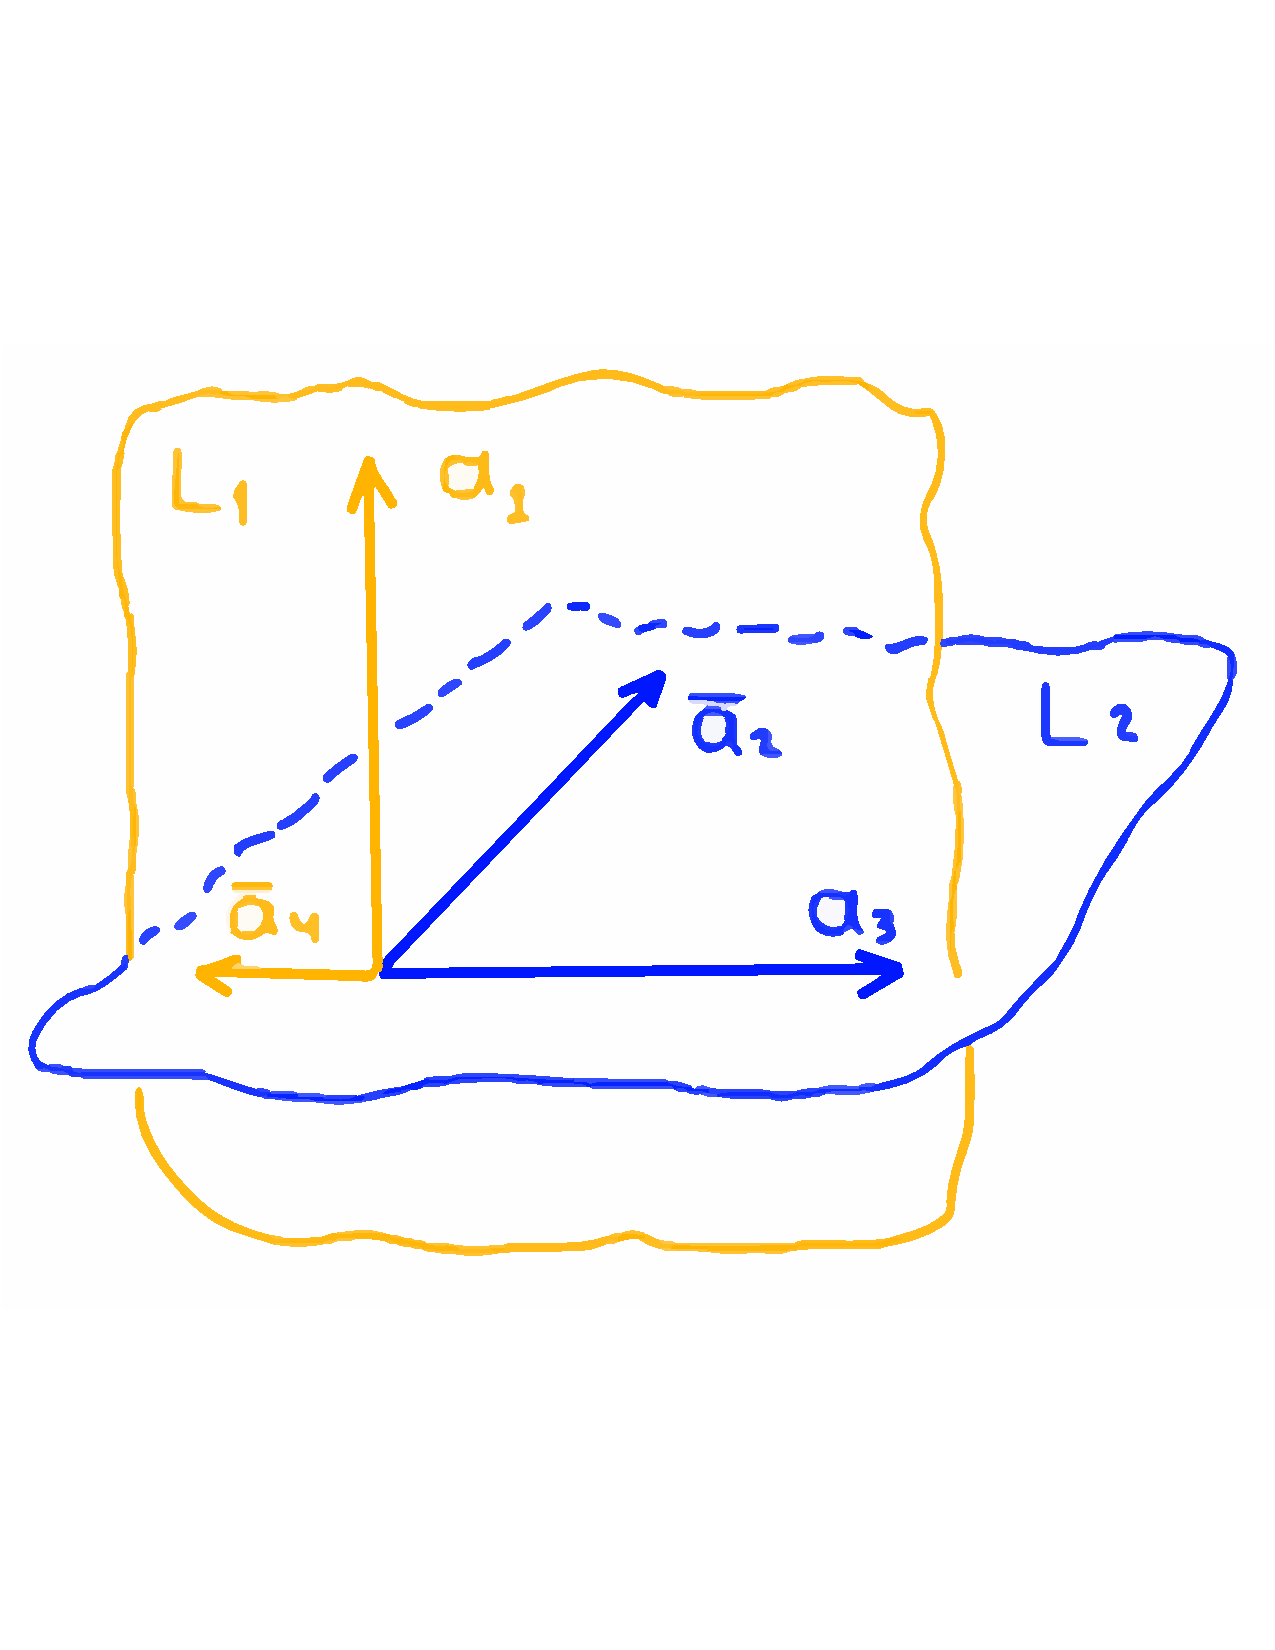
\includegraphics[width=0.8\linewidth]{sem/sem_4/prim_b_cvet} \\ б)}
	\end{minipage}
	\caption{Рисунки подпространств к примерам а) и б)}
	\label{ris:image1}
\end{figure}

\noindent а) ${\color{orange}L_1}\!:~ <\overline{a}_1\!> \qquad \dim L_1 = 1$\\
\phantom{а)}${\color{blue}L_2}\!:~ <\overline{a}_2, \overline{a}_3\!> \qquad \dim L_2 = 2$\\
В данном случае вектора некомпланарны.\\
$L_1+L_2=<\overline{a}_1, \overline{a}_2, \overline{a}_3\!> = \mathbb{R}^3$\\
$\dim (L_1 +L_2) = 3 = \dim L_1 + \dim L_2$\\
Т.о.
$$
L_1+L_2 = L_1 \oplus L_2
$$
%\begin{wrapfigure}{l}{0.3\linewidth}
%	\includegraphics[height=0.2\textheight]{prim_a_cvet}
%	\caption{Рисунок подпространств к примеру а)}
%\end{wrapfigure}
б) ${\color{orange}L_1}\!:~ <\overline{a}_1, \overline{a}_4> \qquad \dim L_1 = 2$\\
${\color{blue}L_2}\!:~ <\overline{a}_2, \overline{a}_3> \qquad \dim L_2 = 2$\\
$L_1+L_2\!:~<\overline{a}_1, \overline{a}_2, \overline{a}_3, \overline{a}_4\!>: \mathbb{R}^3$\\
Но $\dim (L_1+L_2)=3$, т.к. $\overline{a}_4$ можно выкинуть.

В общем случае:
$$
\dim (L_1+L_2) \leq \dim L_1 + \dim L_2
$$
Ответ о размерности даёт \textsf{формула Грассмана}:
$$
\dim (L_1+L_2)=\dim L_1+ \dim L_2 - \dim(L_1\cap L_2).
$$
\section{Понятие проекции вектора на подпространство}
\begin{definition}
	Пусть $\exists a\in L_1,\ b\in L_2, \ x \in L_1+L_2:\ \exists!x = a + b \Leftrightarrow L_1+L_2 = L_1 \oplus L_2$. При этом вектор $a$ называется \textsf{проекцией вектора} $x$ на $L_1$ параллельно $L_2$.  
\end{definition}
\begin{prim}
	Найти проекцию $X(0\ -1\ -1\ 4)^{\text{T}}$ на подпространство $L_1: x_1+x_2+x_3+x_4=0$ вдоль линейной оболочки $L_2\!:~<(1\ -1\ 1\ 0)^{\text{T}}$>.
\end{prim}\\
$L_1: (1\ 1\ 1\ 1\ |\ 0)\Rightarrow
\begin{pmatrix}
x_1\\
x_2\\
x_3\\
x_4\\
\end{pmatrix}
=
\begin{pmatrix*}[r]
-1&-1&-1\\
1&0&0\\
0&1&0\\
0&0&1\\
\end{pmatrix*}
\begin{pmatrix*}[r]
c_1\\
c_2\\
c_3\\
\end{pmatrix*}
$
или
$L_1:
<
\begin{pmatrix*}[r]
-1\\
1\\
0\\
0\\
\end{pmatrix*}
,
\begin{pmatrix*}[r]
-1\\
0\\
1\\
0\\
\end{pmatrix*}
,
\begin{pmatrix*}[r]
-1\\
0\\
0\\
1\\
\end{pmatrix*}
>.
$\\
$
L_2\!:~<\begin{pmatrixr}
1\\-1\\1\\0\\
\end{pmatrixr}>
$\\
Разложим вектор $X$:\\
$$
\begin{pmatrixr}
0\\-1\\-1\\4
\end{pmatrixr}
=\underbrace{
	k
	\begin{pmatrixr}
	1\\-1\\1\\0\\
	\end{pmatrixr}
}_{b\in L_2}
+\underbrace{
	\alpha
	\begin{pmatrixr}
	-1\\1\\0\\0\\
	\end{pmatrixr}
	+\beta
	\begin{pmatrixr}
	-1\\0\\1\\0\\
	\end{pmatrixr}
	+\gamma
	\begin{pmatrixr}
	4\\0\\0\\1\\
	\end{pmatrixr}
}_{a\in L_1}
$$
Очевидно, что это уравнение задает нам СЛУ. Составим ее расширенную матрицу и решим систему:\\
$
\left(\begin{array}{rrrr|r}
1&-1&-1&4&0\\
-1&1&0&0&-1\\
1&0&1&0&-1\\
0&0&0&1&4\\
\end{array}\right)
\rightarrow
\begin{pmatrixr}
k\\\alpha\\\beta\\\gamma\\
\end{pmatrixr}
=
\begin{pmatrixr}
2\\1\\-3\\4\\
\end{pmatrixr}.
$\\
Отсюда легко найти, что
$$
x_{\text{пр}}=
\begin{pmatrixr}
0\\-1\\-1\\4\\
\end{pmatrixr}
-2
\begin{pmatrixr}
1\\-1\\1\\0\\
\end{pmatrixr}
=
\begin{pmatrixr}
-2\\1\\-3\\4\\
\end{pmatrixr}.
$$

\begin{prim}
	Найти размероность и базис суммы подпространств $U_1$ и $U_2$.
	$$
	U_1\!:~<
	\begin{psm}
	1\\0\\-2\\0\\
	\end{psm}
	,
	\begin{psm}
	2\\1\\-1\\1
	\end{psm}
	,
	\begin{psm}
	3\\2\\0\\2
	\end{psm}
	>
	\quad
	U_2:
	\left\{
	\begin{array}{rrrrl}
	x_1&-2x_2&-3x_3&+4x_4&=0\\
	3x_1&+x_2&-2x_3&-2x_4&=0\\
	\end{array}
	\right.
	$$
\end{prim}
$
U_1:
\begin{pmatrixr}
1&0&-2&0\\
2&1&-1&1\\
3&2&0&2\\
\end{pmatrixr}
\xrightarrow[(3)-3(1)]{(2)-2(1)}
\begin{pmatrixr}
1&0&-2&0\\
0&1&3&1\\
0&2&6&2\\
\end{pmatrixr}
$\\
Последняя строка ЛЗ со второй, ее можно вычеркнуть $\Rightarrow \dim U_1 = 2$, базис:
$\left\{
\begin{psm}
1\\0\\-2\\0\\
\end{psm}
,
\begin{psm}
0\\1\\3\\1\\
\end{psm}
\right\}.
$\\
Переведём способ задания $U_2$ из СЛУ в линейную оболочку. Для этого решим эту СЛУ:\\
$
\left(\begin{array}{rrrrr}
1&-2&-3&4&0\\
3&1&-2&-2&0\\
\end{array}\right)
\rightarrow
\left(\begin{array}{rrrrr}
1&0&-1&0&0\\
0&1&1&-2&0\\
\end{array}\right)
$\\
$$
\begin{pmatrixr}
x_1\\x_2\\x_3\\x_4\\
\end{pmatrixr}
=
\begin{pmatrixr}
1&0\\
-1&2\\
1&0\\
0&1\\
\end{pmatrixr}
\begin{pmatrixr}
c_1\\c_2\\
\end{pmatrixr}, \quad \dim U_2 = 2, \quad \text{ базис }U_2:\left\{\begin{pmatrixr}
1\\-1\\1\\0\\
\end{pmatrixr}
,
\begin{pmatrixr}
0\\-2\\0\\1\\
\end{pmatrixr}\right\}.
$$
$
U_1+U_2\!:~<
\begin{psm}
1\\0\\-2\\0
\end{psm}
,
\begin{psm}
0\\1\\3\\1\\
\end{psm}
,\begin{psm}
1\\-1\\1\\0\\
\end{psm}
,
\begin{psm}
0\\2\\0\\1\\
\end{psm}
>.
$\\
$
\begin{pmatrixr}
1&0&1&0\\
0&1&-1&2\\
2&3&1&0\\
0&1&0&1\\
\end{pmatrixr}
\xrightarrow{(3)-(1)}
\begin{pmatrixr}
1&0&-&2&0\\
0&1&3&1\\
0&-1&3&0\\
0&2&0&1\\
\end{pmatrixr}
$\\
3 строка ЛЗ с 2 и 4, ее можно вычеркнуть $\Rightarrow \dim(U_1+U_2) = 3$, базис:
$
\left\{
\begin{psm}
1\\0\\-2\\0\\
\end{psm}
,
\begin{psm}
0\\1\\3\\1\\
\end{psm}
,
\begin{psm}
0\\2\\0\\1\\
\end{psm}
\right\}.
$
\begin{prim}
	В условиях примера 4 найти размерность и базис пересечения.
\end{prim}\\
$\dim  (U_1+U_2)=\dim  U_1+\dim  U_2-\dim (U_1 \cap U_2)$\\
$\dim  (U_1+U_2)=3$, $\dim  U_1=2$, $\dim  U_2=2 \Rightarrow \dim (U_1 \cap U_2)=1$

\noindent\textbf{1 способ}

Зададим $U_1$ как систему: 
$U_1\!:~<\left(
\begin{smallmatrix*}[r]
1\\
0\\
-2\\
0\\
\end{smallmatrix*}
\right) , \left(
\begin{smallmatrix*}[r]
0\\
1\\
3\\
1\\
\end{smallmatrix*}
\right)>$\\
$$
\begin{pmatrix*}[r]
1 & 0 & \vrule & x_1\\
0 & 1 & \vrule & x_2\\
-2 & 3 & \vrule & x_3\\
0 & 1 & \vrule & x_4\\
\end{pmatrix*}
\xrightarrow[(4)-(2)]{ 
	(3)+2(1),
	(3)-3(2)}
\begin{pmatrix*}[c]
1 & 0 & \vrule & x_1\\
0 & 1 & \vrule & x_2\\
0 & 0 & \vrule & x_3+2x_1-3x_2\\
0 & 0 & \vrule & x_4-x_2\\
\end{pmatrix*}
$$\\
$
U_1: 
\left\{	
\begin{array}{rrrrl}
2x_1 & - 3x_2 & + x_3 & & =0 \\
2x_1 & + x_2 & & + x_4 & =0 \\
\end{array}
\right.
$\\
$
U_1 \cap U_2= 
\left\{	
\begin{array}{c}
U_1 \\
U_2 \\
\end{array}
\right.
$\\
$$
\begin{pmatrix*}[r]
1 & 0 & -1 & 0 & \vrule & 0\\
0 & 1 & 1 & -2 & \vrule & 0\\
2 & -3 & -1 & 0 & \vrule & 0\\
0 & -1 & 0 & 1& \vrule & 0\\
\end{pmatrix*}
\Rightarrow
<
\begin{pmatrix*}[c]
1\\
1\\
1\\
1\\
\end{pmatrix*}
> (\text{базис } U_1 \cap U_2)
$$
\textbf{2 способ}\\
Базис $U_1: a_1, a_2$\\
Базис $U_2: b_1, b_2$\\
$P \in U_1, P \in U_2;$ \\
$ P=\alpha_1a_1+\alpha_2a_2=\beta_1b_1+\beta_2b_2 \Rightarrow \alpha_1, \alpha_2 $




\part{Семинар 5. Линейные отображения. Часть 1.}
\section{Определение линейного отображения}
\begin{definition}
	Пусть заданы $L$ и $\overline{L}$ --- два линейных пространства. \textsf{Отображение} $\phi$ из $L$ в $\overline{L}$ --- правило, по которому \underline{каждому} вектору из $L$ ставится в соответствие \underline{единственный} вектор из $\overline{L}$.\\
	Обозначение: $\phi: L\rightarrow\overline{L}$.
\end{definition}

\begin{definition}
	\textsf{Сюрьекция} --- отображение, при котором каждый элемент из $\overline{L}$ является образом вектора из $L$.
\end{definition}

\begin{figure}[h!]
	\centering
	\def\svgwidth{5cm} % если надо изменить размер
	\input{sem/sem_5/surekt.pdf_tex}
	\caption{Сюръективная функция}
	\label{...}
\end{figure}

\begin{definition}
	\textsf{Инъекция} --- отображение, при котором каждый образ из $\overline{L}$ имеет единственный прообраз в $L$.
\end{definition}

\begin{figure}[h!]
	\centering
	\def\svgwidth{5cm} % если надо изменить размер
	\input{sem/sem_5/inekt.pdf_tex}
	\caption{Инъективная функция}
	\label{...}
\end{figure}

\begin{definition}
	Сюрьекция + инъекция = \textsf{биекция} --- это отображение, которое является одновременно и сюръективным, и инъективным (взаимно--однозначное соответствие).
\end{definition}

\begin{definition}
	Если в результате отображения $L=\overline{L}$, то такое отображение называется \textsf{преобразованием}.
\end{definition}

\begin{definition}
	Отображение $\pi$ называется \textsf{линейным}, если выполнено:
	$$
	\left\{
	\begin{array}{l}
	\phi(x+y)=\phi(x)+\phi(y)\\
	\phi(\alpha x)=\alpha\phi(x).\\
	\end{array}\right.
	$$
\end{definition}

Примеры:
\begin{itemize}
	\item аффинные преобразования плоскости
	\item геометрия 3D (т.е. преобразования в трёхмерном пространстве: поворот, симметрия и т.д.)
	\item присвоение координат в линейном пространстве (пространство многочленов $\rightarrow$ пространство столбцов т.е. координатный изоморфизм)
	\item умножение на матрицу, транспонирование
	\item дифференцирование, интегрирование (только для определённого интеграла, чтобы избежать появление константы)
\end{itemize}
Очевидно, что $\phi(0)=0$.

Рассмотрим ЛЗ систему векторов $a_1,\dots,a_n$.
$$
\alpha_1 a_1+\dots+\alpha_n a_n=0.
$$
Подействуем преобразованием $\phi$:
$$
\alpha_1 \phi(a_1)+\dots+\alpha_n \phi(a_n)=0.
$$
Отсюда видно, что \textsf{система образов} --- тоже ЛЗ система векторов с теми же коэффициентами. Но для ЛНЗ системы векторов данное утверждение не верно (контрпример: нуль--преобразование).

\begin{definition}
	\textsf{Образ} $\phi: \im \phi:\{\phi(x)\in \overline{L}:x\in L\}$ --- множество всех образов из $L$ в $\overline{L}$.
\end{definition}

\begin{definition}
	\textsf{Ядро} $\phi: \ker{\phi}: \{x\in L:\phi(x)=0\}$ --- множество векторов из $L$, которые переходят в 0.
\end{definition}

\begin{definition}
	\textsf{Ранг} $\phi: r=\dim(\im{\phi})$ --- размерность образа.
\end{definition}

\begin{wrapfigure}{r}{0.27\linewidth}
	\def\svgwidth{5cm} % если надо изменить размер
	\input{sem/sem_5/prim1.pdf_tex}
	\caption{К примеру 1а}
	\label{...}
\end{wrapfigure}

\begin{prim}
	Работаем в $\mathbb{R}^3$, ОНБ, \textbf{a}$\neq$\textbf{0}, \textbf{n}$\neq$\textbf{0}.\\
	Найти \phi, если \phi --- ортогональная проекция на:\\
	а) $L_1$: \textbf{[r, a] = 0}\\
	б) $L_2$: \textbf{(r, n)} = 0
\end{prim}



\noindent а) $\phi(\textbf{x})=\cfrac{\textbf{(x,\,a)}}{\abs{\textbf{a}}^2}\,\textbf{a}$ --- формула для проекции вектора на прямую (из аналит. геометрии).\\
$\ker \phi : \textbf{(r,\,a)}=0$ --- плоскость, ортогональная вектору $\textbf{a}$.\\
$\im \phi: \textbf{[r,\,a]=0}$.\\
$r = 1$ (прямая).

\begin{wrapfigure}{r}{0.27\linewidth}
	\def\svgwidth{5cm} % если надо изменить размер
	\input{sem/sem_5/prim1b.pdf_tex}
	\caption{К примеру 1б}
	\label{...}
	\vspace{-10cm}
\end{wrapfigure}

\noindent б) $\phi(\textbf{x})=\textbf{x}-\textbf{p}$\\
$\phi(\textbf{x})=\textbf{x}-\cfrac{\textbf{(\textbf{x},\,\textbf{n})}}{\abs{\textbf{n}}^2}\,\textbf{n}$.\\
$\ker \phi: \textbf{[r,\,n]=0}.$\\
$\im \phi: \textbf{(r,\,n)}=0$ (плоскость).\\
$r=2$ (плоскость).

\section{Матрица линейного отображения}
\noindent$\phi: L\rightarrow\overline{L}, \dim L=n<\infty, \dim \overline{L}=m<\infty$\\
Базисы в $L: \textbf{e} (e_1,\dots,e_n)$, в $\overline{L}: \textbf{f} (f_1,\dots,f_m)$, $a \in L$. $\phi(a) \in \overline{L}$.\\
Пусть $a$ имеет в $L$ координатный столбец $\textbf{x}$, а $\phi(a)$ в $\overline{L}$ координатный столбец $\textbf{y}$. Построим такую матрицу $A$: $\underset{m\times n} A\cdot \underset{n\times 1}{\text{\textbf{x}}}=\underset{m\times 1}{\text{\textbf{y}}}$.\\
Пусть $\textbf{x}=e_1: (1\ 0\ \cdots\ 0)^{\text{T}}$.\\
$y=\underset{\text{в базисе $f$}}{\phi(e_1)}=Ae_1=A\cdot (1\ 0\ \cdots\ 0)^{\text{T}}=a_1$ --- первый столбец из A. Аналогично поступим с вторым, третьим и т.д. столбцами. Тогда матрица линейного отображения A имеет вид:
$$A=
\left.\left(\hspace{1mm}
\begin{array}{|c|c|c|}
\cline{1-1} \cline{3-3}
\multirow{4}{*}{$\phi(e_1)$} & \multirow{4}{*}{$\cdots$} & \multirow{4}{*}{$\phi(e_n)$} \\
&                           &                              \\
&                           &                              \\
&                           &                              \\ \cline{1-1} \cline{3-3} 
\end{array}\hspace{1mm}\right) \right\}m
$$
В данном случае, столбцы матрицы --- это координатные столбцы $\phi(e_i)$ в базисе $f$ т.к.:
$$
a=\alpha_1 e_1+\dots+\alpha_n e_n
$$
Подействуем на него преобразованием $\phi$:
$$
\phi(a)=\alpha_1 \phi(e_1)+\dots+\alpha_n \phi(e_n)
$$

В примерах 2--5 вопрос следующий: найти $A$, если задано $\phi$ --- преобразование $\mathbb{R}^3$, в ОНБ.
\begin{prim}
	$\phi$ --- поворот вокруг $\textbf{$e_3$}$ на угол $\frac{\pi}{2}$.
\end{prim}

\begin{wrapfigure}{r}{0.27\linewidth}
	\def\svgwidth{3cm} % если надо изменить размер
	\input{sem/sem_5/prim2.pdf_tex}
	\caption{К примеру 2}
	\label{...}
	\vspace{-9cm}
\end{wrapfigure}

\noindent$\underset{\text{e$_1$,e$_2$,e$_3$}}{L}\rightarrow\underset{\text{e$_1$,e$_2$,e$_3$}}{\overline{L}}$\footnote{Всегда в решении задачи обязательно нужно выбрать базисы.}.\\
$\phi(\textbf{e$_1$})=\textbf{e$_2$}: \begin{psm}
0\\1\\0\\
\end{psm}\\
\phi(\textbf{e$_2$})=-\textbf{e$_1$}: \begin{psm}
-1\\0\\0\\
\end{psm}\\
\phi(\textbf{\text{e$_3$}})=\textbf{e$_3$}:\begin{psm}
0\\0\\1\\
\end{psm}$\\
$$A=\begin{pmatrixr}
0&-1&0\\
1&0&0\\
0&0&1\\	
\end{pmatrixr}$$
Для построения матрицы $A$ нам необходимо и достаточно образов преобразования.
\begin{prim}
	$\phi$ --- ортогональное проецирование на $L: x=y=z$.
\end{prim}

\begin{wrapfigure}{r}{0.35\linewidth}
	\def\svgwidth{6cm} % если надо изменить размер
	\input{sem/sem_5/prim3.pdf_tex}
	\caption{К примеру 3}
	\label{...}
	\vspace{-9cm}
\end{wrapfigure}

\noindent$\underset{\text{e$_1$,e$_2$,e$_3$}}{L}\rightarrow\underset{\text{e$_1$,e$_2$,e$_3$}}{\overline{L}}$\\
$\phi(\textbf{x})=\cfrac{\textbf{(x,\,a)}}{\abs{\textbf{a}}^2}\textbf{a}$\\
<<Прогоним>> через эту формулу все базисные векторы:\\
$\left.
\begin{aligned}
\phi(\textbf{e$_1$})=\frac{1}{3}\begin{psm}
1\\1\\1
\end{psm}\\
\phi(\textbf{e$_2$})=\frac{1}{3}\begin{psm}
1\\1\\1
\end{psm}\\
\phi(\textbf{e$_3$})=\frac{1}{3}\begin{psm}
1\\1\\1
\end{psm}
\end{aligned}
\right\}\Rightarrow A = \cfrac{1}{3}\begin{pmatrixr}
1&1&1\\1&1&1\\1&1&1\\
\end{pmatrixr}
$
\\
\begin{prim}
	$\varphi$ - отражение относительно $\alpha$: $2x-2y+z=0$
\end{prim}\\

\begin{wrapfigure}{r}{0.35\linewidth}
	\vspace{-2.5cm}
	\def\svgwidth{6cm} % если надо изменить размер
	\input{sem/sem_5/prim4.pdf_tex}
	\caption{К примеру 4}
	\label{...}
	\vspace{-9cm}
\end{wrapfigure}

$\underset{\text{e$_1$,e$_2$,e$_3$}}{L}\rightarrow\underset{\text{e$_1$,e$_2$,e$_3$}}{\overline{L}}$\\
$\textbf{n} (2;-2;1)$\\
$|\textbf{n}|^2=9$\\
$\varphi(\textbf{p})=\textbf{p}-2\cfrac{\textbf{(p,\,a)}}{|\textbf{a}|^2}\textbf{n}$\\
$\varphi(\textbf{e$_1$})=
\left(
\begin{smallmatrix*}[r]
1\\ 0\\ 0\\
\end{smallmatrix*}
\right)
-2 \cdot \frac{2}{9} 
\left(
\begin{smallmatrix*}[r]
2\\ -2\\ 1\\
\end{smallmatrix*}
\right)$
;
$\varphi(\textbf{e$_1$})=\frac{1}{9} 
\left(
\begin{smallmatrix*}[r]
1\\ 8\\ -4\\
\end{smallmatrix*}
\right)$;\\
$\varphi(\textbf{e$_2$})=\frac{1}{9} 
\left(
\begin{smallmatrix*}[r]
8\\ -7\\ 4\\
\end{smallmatrix*}
\right)$;\\
$\varphi(\textbf{e$_3$})=\frac{1}{9} 
\left(
\begin{smallmatrix*}[r]
-4\\ 4\\ 1\\
\end{smallmatrix*}
\right)$;\\
$$
A=\frac{1}{9} 
\begin{pmatrix*}[r]
1 & 8 & -4\\
8 & -7 & 4\\
-4 & 4 & 1\\
\end{pmatrix*}
$$\\
\begin{prim}
	$L_1: x=0$\\
	$L_2: 2x=2y=-z$\\
\end{prim}\\

\begin{wrapfigure}{r}{0.4\linewidth}
	\vspace{-2.5cm}
	\def\svgwidth{8cm} % если надо изменить размер
	\input{sem/sem_5/prim5.pdf_tex}
	\caption{К примеру 5}
	\label{...}
	\vspace{-9cm}
\end{wrapfigure}

$\underset{\text{e$_1$,e$_2$,e$_3$}}{L}\rightarrow\underset{\text{e$_1$,e$_2$,e$_3$}}{\overline{L}}$\\

$\varphi$ --- проецирование на $L_1 || L_2$\\
$L_1: \langle
\begin{pmatrix*}[r]
0\\
1\\
0\\
\end{pmatrix*}
,
\begin{pmatrix*}[r]
0\\
0\\
1\\
\end{pmatrix*}
\rangle
$,
$L_2: \langle
\begin{pmatrix*}[r]
\frac{1}{2} \\
\frac{1}{2} \\
-1\\
\end{pmatrix*}
\rangle$\\
$ \textbf{p}=
\underbrace{
	\alpha
	\left(
	\begin{smallmatrix*}[r]
	0\\ 1\\ 0\\
	\end{smallmatrix*}
	\right)
	+\beta
	\left(
	\begin{smallmatrix*}[r]
	0\\ 0\\ 1\\
	\end{smallmatrix*}
	\right)
}_{\in L_1}
+
\underbrace{
	\gamma
	\left(
	\begin{smallmatrix*}[r]
	\frac{1}{2} \\
	\frac{1}{2} \\
	-1\\
	\end{smallmatrix*}
	\right)
}_{\in L_2}\\
\textbf{e$_1$}: 
\begin{psm}
1\\ 0\\ 0\\
\end{psm}
=
\underbrace{
	\alpha
	\left(
	\begin{smallmatrix*}[r]
	0\\ 1\\ 0\\
	\end{smallmatrix*}
	\right)
	+\beta
	\left(
	\begin{smallmatrix*}[r]
	0\\ 0\\ 1\\
	\end{smallmatrix*}
	\right)
}_{\varphi(\textbf{e$_1$})}
+\gamma
\left(
\begin{smallmatrix*}[r]
\frac{1}{2} \\
\frac{1}{2} \\
-1\\
\end{smallmatrix*}
\right)
\Rightarrow
\gamma=2
\Rightarrow
\varphi(\textbf{e$_1$})=
\left(
\begin{smallmatrix*}[r]
0\\ -1\\ 2\\
\end{smallmatrix*}
\right)
$\\
$\textbf{e$_2$}: \varphi(\textbf{e$_2$})=\textbf{e$_2$};\\
\textbf{e$_3$}: \varphi(\textbf{e$_3$})=\textbf{e$_3$}.  $\\
Ответ:$
\begin{pmatrix*}[r]
0 & 0 & 0\\
-1 & 1 & 0\\
2 & 0 & 1\\
\end{pmatrix*}
$\\
Понимая пример 5 как отображение, можно заметить, что $\dim(\im\varphi)=2$,  а значит, для описания всевозможных результатов в $\bar L$ можно было выбрать базис из двух векторов.\\
$ f= \left\{ \left(
\begin{smallmatrix*}[r]
0\\ 1\\ 0\\
\end{smallmatrix*}
\right) 
, 
\left(
\begin{smallmatrix*}[r]
0\\ 0\\ 1\\
\end{smallmatrix*}
\right) 
\right\}$\\ 
$\varphi (\textbf{e$_1$})=\left(
\begin{smallmatrix*}[r]
-1\\ 2\\
\end{smallmatrix*}
\right) $
,
$\varphi (\textbf{e$_2$})=\left(
\begin{smallmatrix*}[r]
1\\ 0\\
\end{smallmatrix*}
\right) $
,
$\varphi (\textbf{e$_3$})=\left(
\begin{smallmatrix*}[r]
0\\ 1\\
\end{smallmatrix*}
\right) $;\\
$$A=
\begin{pmatrixr}
-1 & 1 & 0\\
2 & 0 & 1\\
\end{pmatrixr}
$$
\begin{prim}
	$ \varphi : \underset{\textbf{e$_1$}, \textbf{e$_2$}, \textbf{e$_3$}}L \Rightarrow \underset{\textbf{f$_1$}, \textbf{f$_2$}, \textbf{f$_3$}, \textbf{f$_4$}}{\bar L} $\\
	
	$L: \langle\underset{=\text{\textbf{$e_1$}}}1, \underset{=\text{\textbf{$e_2$}}}x, \underset{=\text{\textbf{$e_3$}}}{x^2}\rangle$ , 
	$L: \langle\underset{=\text{\textbf{$f_1$}}}1, \underset{=\text{\textbf{$f_2$}}}x, \underset{=\text{\textbf{$f_3$}}}{x^2}, \underset{=\text{\textbf{$f_4$}}}{x^3}\rangle$ \\
\end{prim}
$\varphi (x)=\int\limits^x_0 f(t)dt$\\
$$
\left.
\begin{aligned}
\varphi (e_1)=\int\limits^x_0 1 dt=x
\left(
\begin{smallmatrix*}[r]
0\\ 1\\ 0\\ 0\\
\end{smallmatrix*}
\right) \\
\varphi (e_2)=\int\limits^x_0 t dt=\frac{x^2}{2}
\left(
\begin{smallmatrix*}[r]
0\\ 0\\ \frac{1}{2}\\ 0\\
\end{smallmatrix*}
\right) \\
\varphi (e_3)=\int\limits^x_0 t^2 dt=\frac{x^3}{3}
\left(
\begin{smallmatrix*}[r]
0\\ 0\\  0\\ \frac{1}{3}\\
\end{smallmatrix*}
\right) 
\end{aligned}
\right\}
A=
\begin{pmatrix*}[r]
0 & 0 & 0\\
1 & 0 & 0\\
0 & \frac{1}{2} & 0\\
0 & 0 & \frac{1}{3}\\
\end{pmatrix*}
$$





\part{{Семинар 6. Линейные отображения. Часть 2.}\\}
Для начала решим небольшой пример по прошлому семинару.
\begin{prim}
	$\phi: M_{2\times 2}\rightarrow M_{2\times 1}, \phi(\textbf{x})=\textbf{x}\begin{psm}
	1\\4\\
	\end{psm}$. Найти матрицу линейного преобразования $A$.
\end{prim}\\

Запишем базисы:\\
$M_{2\times 2}: \textbf{e}
\left\{
\begin{psm}
1&0\\
0&0\\
\end{psm}
,
\begin{psm}
0&1\\
0&0\\
\end{psm}
,
\begin{psm}
0&0\\
1&0\\
\end{psm}
,
\begin{psm}
0&0\\
0&1\\
\end{psm}
\right\}\\
M_{2\times1}: \textbf{f}
\left\{
\begin{psm}
1\\0
\end{psm}
,
\begin{psm}
0\\1
\end{psm}
\right\}.
$\\
Для удобства в общем виде найдём, что значит наше преобразование:\\
$$
\phi(\textbf{x})=\begin{pmatrixr}
a&b\\
c&d\\
\end{pmatrixr}
\begin{pmatrixr}
1\\4
\end{pmatrixr}
=
\begin{pmatrixr}
a+4b\\c+4d
\end{pmatrixr}.
$$
Далее <<прогоним>> через преобразование базис \textbf{e}:\\
$
\phi(\textbf{e$_1$})=
\begin{psm}
1&0\\
0&0\\
\end{psm}
\begin{psm}
1\\4
\end{psm}
=
\begin{psm}
1\\0
\end{psm}, \quad
\phi(\textbf{e$_2$})=\begin{psm}
4\\0
\end{psm}, \quad
\phi(\textbf{e$_3$})=\begin{psm}
0\\1
\end{psm}, \quad
\phi(\textbf{e$_4$})=\begin{psm}
0\\4
\end{psm}.
$\\
Отсюда, получаем ответ:
$$
A=\begin{pmatrixr}
1&4&0&0\\
0&0&1&4\\
\end{pmatrixr}.
$$
\section{Рассмотрение ядра и образа}
Рассмотрим $\phi: \underset{\dim L=n}{L}\rightarrow \underset{\dim \overline{L}=m}{\overline{L}}$.\\
Ядро: $\ker\phi: \{\textbf{x} \in L: A\textbf{\textbf{x}}=\textbf{o}\}$\\
Очевидно, что ЛНЗ решения такого уравнения формируют ФСР, а ФСР задаёт линейное подпространство. Вспоминая количество столбцов в ФСР, легко получить формулу:
\begin{equation}
\boxed{\dim\ker\phi=n-\Rg A}.
\label{ker}
\end{equation}
Образ $\im\phi: \{\textbf{y} \in \overline{L}:\exists \textbf{x}\in L: A\textbf{x}=\textbf{y}\}$.\\
Аналогично $\im\phi \in \overline{L}$ формирует линейное подпространство т.к.
\begin{center}
	$
	A\textbf{x$_1$}+A\textbf{x$_2$}=A(\textbf{x$_1$}+\textbf{x$_2$})$
	
	$A\alpha \textbf{x}=\alpha A\textbf{x}$.
\end{center}
Выберем в $L$ базис $\textbf{e}:\{\textbf{e$_1$}, \textbf{e$_2$}, \dots, \textbf{e$_n$}\}$.\\
$\forall \textbf{x} \in L: \textbf{x}=\alpha_1\textbf{e$_1$}+\dots+\alpha_n\textbf{e$_n$} \leftarrow \phi$ (это обозначение значит <<подействуем преобразованием $\phi$>>)\\
$\phi(\textbf{x})=\alpha_1 \underset{=\textbf{a$_1$}}{\phi(\textbf{e$_1$})}+\dots+\alpha_n \underset{=\textbf{a$_n$}}{\phi(\textbf{e$_n$})}=\langle \textbf{a$_1$},\dots, \textbf{a$_n$}\rangle$.\\
Заметим, что $\textbf{a$_1$},\dots, \textbf{a$_n$}$ --- столбцы матрицы $A$. Отсюда следует формула:
\begin{equation}
\boxed{\dim\im\phi=\Rg A=r}.
\label{im}
\end{equation}
Сложим формулы \eqref{ker} и \eqref{im} и получим:
\begin{equation}
\boxed{\dim\ker\phi+\dim\im\phi=n}.
\end{equation}
\begin{center}
	В примерах 2--5: $L=\mathbb{R}^4, \overline{L}=\mathbb{R}^3, A=\begin{psm}
	0&0&2&-2\\
	2&-4&1&1\\
	-1&2&1&-2\\
	\end{psm}$.
\end{center}
\begin{prim}
	Найти образ $\textbf{x}=\begin{psm}
	1\\1\\1\\1\\
	\end{psm}$.
\end{prim}\\

$\phi: A\textbf{x}=\textbf{y}$, т.е. нужно перемножить матрицу $A$ и вектор $\textbf{x}$.\\
$
\begin{psm}
0&0&2&-2\\
2&-4&1&1\\
-1&2&1&-2\\
\end{psm}
\begin{psm}
1\\1\\1\\1
\end{psm}
=
\begin{psm}
0\\0\\0
\end{psm}
=\textbf{o}
\Rightarrow$ ядро не пусто.
\begin{prim}
	Найти прообраз $\textbf{y}=\begin{psm}
	4\\0\\3
	\end{psm}.$
\end{prim}\\

Итак $\phi: \underline{A}\textbf{x}=\underline{\textbf{y}}$. Мы знаем то, что подчёркнуто. Очевидно, что мы получили СЛУ относительно \textbf{x}. Решим ее.
\\
$\left(\begin{array}{rrrr|r}
0 & 0 & 2 & -2 & 4   \\
2 & -4& 1&1&0\\
-1&2&1&-2&3
\end{array}\right)\xrightarrow[(1)\leftrightarrow(3)]{(3)\cdot0.5;(1)\cdot(-1)} \left( \begin{array}{rrrr|r}
-1&2&1&-2&3   \\
2 & -4& 1&1&0\\
0&0&1&-1&2
\end{array}\right) \xrightarrow{(2)-2(1)} \left( \begin{array}{rrrr|r}
-1&2&1&-2&3   \\
0 & 0& 3&-3&6\\
0&0&1&-1&2
\end{array}\right) 
\rightarrow\\
\xrightarrow{(1)+(2)} 
\begin{matrix}
\overset{
	\left(\begin{array}{rrrr|r} % приписывание иксов в матрице!??!?!?!
	1&-2&0&1&-1   \\
	0&0&1&-1&2 \\
	\end{array}\right)
}{
	\begin{matrix*}
	x_1&x_2&x_3&x_4& \ \ \ \ \ 
	\end{matrix*}
}
\end{matrix}
\rightarrow 
\begin{matrix}
\overset{\left(\begin{array}{rrrr|r}
	1&0&-2&1&-1   \\
	0&1&0&-1&2 \\
	\end{array}\right)
}{
	\begin{matrix*}
	x_1&x_3&x_2&x_4& \ \ \ \ \ 
	\end{matrix*}
}
\end{matrix}$
\vspace{3mm}

$\left( \begin{array}{r}
x_1\\
x_3\\
x_2\\
x_4
\end{array}\right) = \left( \begin{array}{r}
-1\\
2\\
0\\
0
\end{array}\right) + \left( \begin{array}{rr}
2 & -1\\
0&1\\
1&0\\
0&1
\end{array}\right) \left( \begin{array}{r}
c_1\\
c_2
\end{array}\right)$
\vspace{3mm}

$\left( \begin{array}{r}
x_1\\
x_2\\
x_3\\
x_4
\end{array}\right) = \left( \begin{array}{r}
-1\\
0\\
2\\
0
\end{array}\right) + \left( \begin{array}{r}
2\\
1\\
0\\
0
\end{array}\right) c_1 + \left( \begin{array}{r}
-1\\
0\\
1\\
0
\end{array}\right) c_2 $

\begin{prim}
	Найти ядро отображения.
\end{prim}\\

Для этого нужно решить СЛУ $A\textbf{x}=\textbf{o} \Rightarrow$

$\Rightarrow\ker\varphi:\langle \left( \begin{array}{r} % МАТФУНКЦИИ
2\\
1\\
0\\
0
\end{array}\right), \left( \begin{array}{r}
-1\\
0\\
1\\
0
\end{array}\right)\rangle$\footnote{В примере 2 как раз и был вектор из $\ker\phi$}, \quad $\dim\ker\phi=2$.

\begin{prim}
	Найти образ $\im\varphi$.
\end{prim}\\

$\im\varphi : \langle \left( \begin{array}{r}
0\\
2\\
-1
\end{array}\right),\left( \begin{array}{r}
0\\
-4\\
2
\end{array}\right),\left( \begin{array}{r}
2\\
1\\
1
\end{array}\right),\left( \begin{array}{r}
-2\\
1\\
-2
\end{array}\right) \rangle$

$A = \begin{pmatrixr}
0 & 2 & -1\\
0 & -4 & 2\\
2 & 1 & 1\\
-2&1&-2\\ \end{pmatrixr}$ \\
Очевидно, что $(2) = -2(1), (4) = (3)+(1) \Rightarrow$ 2 и 4 строку можно вычеркнуть. \\
$\im\varphi :\langle \left( \begin{array}{r}
0\\
2\\
-1
\end{array}\right), \left( \begin{array}{r}
2\\
1\\
1
\end{array}\right) \rangle$\\
$\dim \im\varphi = 2$\\
$\dim \im \varphi +\dim \ker \varphi =4$




\section{Два важных частных случая}

\begin{enumerate}
	\item Если \underline{$\dim\ker\varphi=0$}:
	
	$\dim \im \varphi = n = \Rg A \Rightarrow$ (столбцы ЛНЗ)
	
	$\textbf{y} \in \overline{L}$
	$\ker\varphi = {0}$\\
	Пусть $\textbf{y}=A\textbf{x$_1$}=A\textbf{x$_2$}$
	
	$A(\textbf{x$_1$}-\textbf{x$_2$}) = 0 \Rightarrow \textbf{x$_1$} - \textbf{x$_2$} \in \ker\varphi =\{0\} \Rightarrow \textbf{x$_1$}=\textbf{x$_2$}$
	
	Если $\ker\varphi = \{0\}$, то это \underline{инъекция}.
	
	Оказывается, верно и обратное:
	
	Отображение инъективно $\Leftrightarrow$ $\ker\varphi = {0}$
	
	Докажем в другую сторону:
	
	Пусть $\dim\ker \varphi \geq 1  \Rightarrow \exists \textbf{x$_0$} \neq 0 \in \ker \varphi$
	
	$A\textbf{x}=\textbf{y}$
	
	$A(\textbf{x}+\textbf{x$_0$}) = A\textbf{x}+A\textbf{x$_0$} = \textbf{y}$~---~противоречие инъекции $\Rightarrow \ker\varphi = \{0\}$
	
	Число прообразов = $0, 1, \infty$
	\item Если \underline{$\im\varphi = \mathbb{R}^m = \overline{L}$}:
	
	$\dim \im\varphi = m = \Rg A$~---~строки ЛНЗ $\leftarrow$ \underline{сюръекция}
\end{enumerate}
Биекция $=$ сюръекция $+$ инъекция\\
$\Rg A=n=m$\\
Т.о. \textbf{биекция задаётся невырожденной матрицей}. В таком случае
$$\dim L = \dim \overline L$$
\textsf{Изоморфизм}~--- биективное линейное отображение.\\
Если существует изоморфизм $L \to \overline L$, то говорят, что $L$ и $\overline L$ \textsf{изоморфны}.

\begin{theorem}
	$L$ и $\overline L$ изоморфны$\iff \dim L =
	\dim \overline L$.
\end{theorem}

Для изоморфизма $\exists$ $\varphi^{-1}$ --- \textsf{обратное отображение}, его матрица $A^{-1}$.

\begin{prim}
	Доказать, что отображение $\varphi(f(x)) = 2f(x) + f'(x)$~--- изоморфизм
	в пространстве $P_2$~---  многочленов степени не выше~$2$. Найти $\varphi^{-1}$.
\end{prim}\\

Стандартный базис $L\colon\{ 1, x, x^2 \}$, где $\textbf{e$_1$}=1$, $\textbf{e$_2$}=x$, $\textbf{e$_3$}=x^2$.\\
Общий вид $f(x) = ax^2 + bx + c$,
$\dim L = 3$.
\begin{gather*}
\varphi(f(x)) = 2ax^2 + 2bx + 2c + 2ax + b =
2ax^2 + (2a + 2b)x + (b + 2c),
\quad
\overline L\colon\{ 1, x, x^2 \}
\end{gather*}
$$
\left.
\begin{aligned}
\varphi (e_1)=2
\left(
\begin{smallmatrix}
2\\ 0\\ 0\\
\end{smallmatrix}
\right) \\
\varphi (e_2)=2x+1
\left(
\begin{smallmatrix}
1\\ 2\\ 0\\
\end{smallmatrix}
\right) \\
\varphi (e_3)=2x^2+2x
\left(
\begin{smallmatrix}
0\\ 2\\ 2\\
\end{smallmatrix}
\right) 
\end{aligned}
\right\}
\Rightarrow
A=
\begin{pmatrix}
2 & 1 & 0\\
0 & 2 & 2\\
0 & 0 & 2\\
\end{pmatrix}
$$
$\Rg=3 \Rightarrow$ изоморфизм. Найдем $A^{-1}$:
\begin{gather*}
A^{-1} = \frac{1}{4} \begin{pmatrix} 2 & -1 & 1 \\ 0 & 2 & -2 \\
0 & 0 & 2 \end{pmatrix}.
\end{gather*}
Ответ: $\varphi^{-1} \colon A^{-1} = \cfrac{1}{4} \begin{pmatrix} 2 & -1 & 1 \\ 0 & 2 & -2 \\
0 & 0 & 2 \end{pmatrix}$.

\section{Матрица отображения в новых базисах.}
Пусть в $L$ и $\overline L$ выбраны базисы $\textbf{e}$ и $\textbf{f}$, задано отображение $\varphi\colon L \to \overline L: A$.
Поменяем базисы: $ \textbf{e}' = \textbf{e} S$, $ \textbf{f}' = \textbf{f} P$.
Найдём $A'$:\\
\begin{gather*}
\textbf{x} \in L,~ \textbf{x}=\left(\begin{smallmatrix}
\xi_1 \\ \vdots\\ \xi_n\\
\end{smallmatrix} \right)=\bm{\xi};~~~~~~
\textbf{y} \in L,~ \textbf{y}=\left(\begin{smallmatrix}
\eta_1 \\ \vdots\\ \eta_n\\
\end{smallmatrix} \right)=\bm{\eta}
\end{gather*}
Из теории отображений: $\bm{\eta} = A \bm{\xi};~~~\bm{\eta}' = A' \bm{\xi}';$\\
Из замены базиса: $	\bm{\eta} = P \bm{\eta}';~~~	\bm{\xi} = S \bm\xi';$

\begin{gather*}
P \bm \eta' = A \bm \xi = AS \bm\xi'
\Rightarrow
\bm\eta' = P^{-1} A S \bm\xi'=A' \bm \xi'
\Rightarrow
\boxed{A' = P^{-1} A S.}
\end{gather*}
Если $\varphi$~--- преобразование, то $P=S$ и $A'=S^{-1}AS$\\

\begin{prim} 
	Дано преобразование $\varphi\colon A = \begin{pmatrix} 0 & 2 \\ -1 & -3 \end{pmatrix}$ в базисе $\bf e$. Смена базиса: $\bf e' = \bf e \begin{pmatrix} 2 & 1 \\ -1 & -1 \end{pmatrix}$.
	Найти $A'$.\\
	
	Воспользуемся $A'=S^{-1}AS$. Посчитаем $S^{-1}$:\\
	$$S^{-1} =
	\begin{pmatrix} 1 & 1 \\ -1 & 2 \end{pmatrix}$$.
\end{prim}
$$
A'=
\begin{pmatrix*}[r]
1 & 1\\
-1 & 2\\
\end{pmatrix*}
\begin{pmatrix*}[r]
0 & 2\\
-1 & -3\\
\end{pmatrix*}
\begin{pmatrix*}[r]
2 & 1\\
-1 & -1\\
\end{pmatrix*}
=
\begin{pmatrix*}[r]
-1 & 0\\
0 & -2\\
\end{pmatrix*}
$$
\section{Линейные функции}
\begin{definition}
	\textsf{Функция} $f(x)$ на линейном пространстве $L$ --- правило, которое $\forall x \in L$ ставит в соответствие $f(x) \rightarrow \mathbb{R} $.
	
	Функция $f$ линейная, если 
	$$
	\left\{
	\begin{array}{rl} % некрасивое выравнивание 
	f(x+y)&=f(x)+f(y)\\
	f(\alpha x)&=\alpha f(x)\\
	\end{array}
	\right.
	$$
\end{definition}


Это частный случай линейного отображения при $m=1$.\\
Примеры:\\ % enumerate, не стал исправлять
а) Присвоить вектору его $i$-тую координату.\\
б) Скалярное произведение \textbf{(\textbf{x}, \textbf{a})}, где \textbf{a} --- фиксированный вектор в $\mathbb{R}^3$.\\
в) Определённый интеграл.\\

$\underset{1 \times n}A$- строка функции $A=(\varphi_1 \cdots \varphi_n)$, где $\varphi_i$ --- образ $i$-го базисного вектора (т.е. $\varphi_i=\varphi$(\textbf{e$_i$}))\\

Линейные функции образуют линейное пространство.

\begin{prim}
	Может ли $ \forall x \in L$ выполняться:\\
	а) $f(x)>0$? Ответ: нет, так как нет нуля;\\
	б) $f(x)\geq 0$? Ответ: только если $f(x)\equiv0$;\\
	в) $f(x)=\alpha $? Ответ: только для $\alpha\equiv0$, $f(x)\equiv0$.\\
\end{prim}
\begin{prim}
	$P(t)$ ---  многочлен степени $\leq n$, $f(P(t))=P'(1)$. Найти $A$.
\end{prim}\\

Базис: $\{ 1, t,\cdots, t^n\}$\\
$$
\begin{array}{rl}
\varphi (\text{\textbf{e$_1$}})=&0\\
\varphi (\text{\textbf{e$_2$}})=&1\\
\varphi (\text{\textbf{e$_3$}})=&2\\
\hdotsfor{2}\\
\varphi (\text{\textbf{e$_{n+1}$}})=&n\\
\end{array}
$$
Отсюда получаем ответ:
$$A=
\begin{pmatrix*}[r]
0 & 1 & 2 & \cdots & n\\
\end{pmatrix*}$$
\section{Инвариантные подпространства}
\underline{Будем работать только с преобразованиями.} %22:15
\subsection{Определение}
\begin{definition}
Подпространство $L' \subset L$ называется \textsf{инвариантным} \textbf{относительно преобразования $\bm\phi$}, если
$$
\forall \textbf{x} \in L' \mapsto \phi(\textbf{x}) \in L'\text{ или }\phi(L')\subset L'.
$$
\end{definition}
Например:
\begin{itemize}
	\item \textbf{o}, L --- вырожденные случаи.
	\item Поворот $\mathbb{R}^3$ вокруг \textbf{e$_3$} на $\pi/2$ (рис. \ref{prim1}). Инвариантные подпространства: $\textbf{o}, \mathbb{R}^3, \langle \textbf{e$_1$}, \textbf{e$_2$} \rangle, \langle \textbf{e$_3$}\rangle$.
	\item Ядро преобразования $\phi \ (\ker \phi)$ всегда инвариантно относительно этого преобразования $\phi$.
	\item $\im \phi$
	\begin{theorem}
	Если какое-то подпространство содержит в себе образ, то $L'$ инвариантно относительно $\phi$.
	\end{theorem}
	\begin{proof}
		$$\forall \textbf{x} \in L' \mapsto \phi(\textbf{x}) \subset \im\phi\subset L'$$
	\end{proof}
\end{itemize}
\subsection{Свойства инвариантных подпространств}
\begin{predlog}
	Сумма инвариантных подпространств инвариантна.
\end{predlog}
\begin{proof}
	$$
	\left.
	\begin{array}{r}
		\textbf{x} \in L_1, \phi(\textbf{x}) \in L_1\\
		\textbf{y} \in L_2, \phi(\textbf{y}) \in L_2\\
	\end{array}
	\right\} \Rightarrow \phi(\textbf{x}) + \phi(\textbf{y}) \in L_1 + L_2
	$$
\end{proof}
\begin{predlog}
	Пересечение инвариантных подпространств инвариантно.
\end{predlog}
\begin{proof}
	$$
	\left.
	\begin{array}{r}
	\textbf{x} \in L_1, \phi(\textbf{x}) \in L_1\\
	\textbf{x} \in L_2, \phi(\textbf{x}) \in L_2\\
	\end{array}
	\right\} \Rightarrow \phi(\textbf{x}) \in L_1 \cap L_2
	$$
\end{proof}
\section{Матрица преобразования}
\subsection{Вид матрицы преобразования}
Рассмотрим линейное пространство $L$, $\dim L=n$. Пусть $L' \subset L$, $\dim L' = k$ --- инвариантное подпространство относительно $\phi$, базис в $L': \{\textbf{e$_1$}, \dots, \textbf{e$_k$}\}$, базис в $L: \{\textbf{e$_1$}, \dots, \textbf{e$_k$}, \textbf{e$_{k+1}$}, \dots, \textbf{e$_n$}\}$. %22:44 23:10

\begin{figure}
	\centering
	\def\svgwidth{5cm} % если надо изменить размер
	\input{sem/sem_7/podpr.pdf_tex}
	\caption{Подпространство в L}
	\label{podpr}
\end{figure}

Напомним, что матрица преобразования $A$ строится из образов базисных векторов:
$$A=
\left(\hspace{1mm}
\begin{array}{|c|c|c|}
\cline{1-1} \cline{3-3}
\multirow{4}{*}{$\phi(e_1)$} & \multirow{4}{*}{$\cdots$} & \multirow{4}{*}{$\phi(e_n)$} \\
&                           &                              \\
&                           &                              \\
&                           &                              \\ \cline{1-1} \cline{3-3} 
\end{array}\hspace{1mm}\right)
$$
Т.о. матрица преобразования в выбранном базисе имеет следующий вид:
$$
A =\left(
\begin{tabular}{c|c}
$A_1$ & $A_2$\\
\hline
$O$ & $A_4$\\
\end{tabular}
\right)^{\square}\text{ --- \textsf{клетчочно--треугольный вид}.}\footnote{Квадрат над матрицей значит, что матрица блочная.}
$$

Пусть теперь $L=L_1\oplus L_2 \oplus \dots \oplus L_s, \forall i\ L_i$ --- инвариантное подпространство относительно $\phi$.

\begin{figure}[h!]
	\centering
	\def\svgwidth{10cm} % если надо изменить размер
	\input{sem/sem_7/summa.pdf_tex}
	\caption{Прямая сумма подпространств}
	\label{summa}
\end{figure}

Тогда матрица преобразования имеет вид:
$$
A =\left(
\begin{array}{cccc}\cline{1-1}
\multicolumn{1}{|c|}{A_1} & O & \dots & O\\\cline{1-1} \cline{2-2}
O & \multicolumn{1}{|c|}{A_2} &\dots& O\\\cline{2-2}
\vdots&\vdots&\ddots&\vdots\\\cline{4-4}
O & O &\dots & \multicolumn{1}{|c|}{A_s}\\\cline{4-4}
\end{array}
\right)^{\square}\text{ --- \textsf{клеточно--диагноальный вид}.}
$$
Ширина и высота каждой клетки равны размерности инвариантного подпространства.
\begin{prim} %\begin{prim} !!!
	Найти инвариантные подпространства в $\mathbb{R}^3$ относительно $\varphi$. %подпрострашнства, R^3!!!!
\end{prim}\\

\begin{wrapfigure}{r}{0.27\linewidth}
	\def\svgwidth{3cm} % если надо изменить размер
	\input{sem/sem_7/prim2.pdf_tex}
	\caption{К примеру 1}
	\label{prim1}
	\vspace{-1cm}
\end{wrapfigure}

$A = \left( \begin{array}{rr|r} % ВЫРАВНИВАНИЕ
0&-1&0\\
1&0&0\\ 
\hline
0&0&1
\end{array} \right)$

Из вида $A$ видно, что существует два не пересекающихся инвариантных подпространства.\\
$\textbf{o}, \mathbb{R}^3, \langle \textbf{e$_1$}, \textbf{e$_2$} \rangle, \langle \textbf{e$_3$} \rangle.$\\ % Векторы жирным!!!!!  

\subsection{Геометрический смысл матрицы преобразования}
Поговорим о геометрии. Научимся определять по внешнему виду матрицы ее геометрический смысл.

$\left( \begin{array}{rrr}
1 & 0 & 0  \\
0 & 1& 0\\
0&0&-1
\end{array}\right)$~---~отражение относительно $\langle \textbf{e$_1$}, \textbf{e$_2$} \rangle.$ %Точки в конце предложений надо ставить!

$\left( \begin{array}{rrr}
1 & 0 & 0  \\
0 & 1& 0\\
0&0&0
\end{array}\right)$~---~проекция.
%Меньше \vspace{}

$\left( \begin{array}{rrr}
1 & 0 & 0  \\
0 & 3& 0\\
0&0&1
\end{array}\right)$~---~растяжение вдоль $\textbf{e$_2$}$ в 3 раза.\\

Нам интересны матрицы вида:

$A=\left( \begin{array}{ccc} %Здесь выравниваение пришлось оставить из-за того, что выравниваение по правому краю происходит по индексам, что выглядит ужасно
\lambda_1 & 0 & 0  \\
0 & \lambda_2& 0\\
0&0&\lambda_3
\end{array}\right)$~---~ обобщённое растяжение $\Leftrightarrow \varphi(\textbf{e$_i$}) = \lambda_i\textbf{e$_i$}$.

\section{Собственный вектор}
\subsection{Определение}
Рассмотрим преобразование  $\varphi$ с матрицей $A$, тогда ненулевой вектор $\textbf{x}$ называется \textsf{собственным вектором}, если  $\varphi(\textbf{x}) = \lambda \textbf{x}$; $\lambda$~---~собственное значение. %Точки в конце предложений!!! + лучше выделять не почеркиванием, а рубленым шрифтом + векторы жирным!!!

Множество собственных векторов, отвечающих одному и тому же собственному значению, образует \textsf{собственное пространство}.
\subsection{Свойства}
\begin{predlog} % Оформление под теорему!
	Собственный вектор (и только он) порождает одномерное инвариантное подпространство. % "Собственный вектор (и только он) порождает одномерное инвариантно пространство" - я конечно все понимаю, но "инвариантно пространство" ни в какие ворота, так еще и породить пространство он ну никак не может.
\end{predlog}
\begin{proof}
	Рассмотрим инвариантное подпространство  $\langle \textbf{x} \rangle \Rightarrow \varphi(\alpha \textbf{x}) = \alpha \varphi(\textbf{x}) = \alpha\lambda \textbf{x} \in~\langle \textbf{x}\rangle$.
\end{proof}
\section{Алгоритм поиска собственных значений и собственных векторов}
\vspace{-0.5cm}
$$\varphi(\textbf{x}) = \lambda \textbf{x}$$
$$\varphi(\textbf{x}) - \lambda \textbf{x} = \textbf{o}$$
Рассмотрим тождественное преобразование $Id$, матрица его преобразования $E$. % Без сокращений!!!
$$(\varphi -\lambda Id)(\textbf{x})=\textbf{o}$$
Перейдём к матричному виду:
\begin{equation}
(\varphi -\lambda E)\textbf{x}=\textbf{o} \tag{$*$}
\end{equation}
Итак, мы получили СЛУ размеров $n\times n$. Она имеет либо одно решение (нулевое), но оно нам не интересно, т.~к. $\textbf{x}\neq\textbf{o}$, либо бесконечно много решений $\Rightarrow A$ должна быть вырожденной $\Rightarrow \det(A-\lambda E) = 0 \rightarrow \lambda_i\text{ --- cобственное значение} \rightarrow (*) \rightarrow \textbf{x}\text{ --- cобственный вектор}.$ %ТОЧКА!, тире ---!!!!
\begin{prim}
	Найти собственные значения и собственные векторы.\\
	$$A = \left( \begin{array}{rrr}
	2 & 2 & 1  \\
	-2 & -3& 2\\
	3&6&0
	\end{array}\right)
	$$
\end{prim}\\

Найдём $\lambda$ из условия $\det(A-\lambda E) = 0$:

$\begin{array}{|ccc|}
2-\lambda & 2 & 1  \\
-2 & -3 -\lambda& 2\\
3&6&-\lambda
\end{array} = 0 = -\lambda^3- \lambda^2+17\lambda -15 \Rightarrow \lambda_1 =1, \lambda_2 =3, \lambda_3 = -5$\\
Далее подставим числа $\lambda$ в $(*)$:

\begin{enumerate}
	\item{
		$\lambda_1=1 :$
		$\begin{pmatrix*}[r]
		1 & 2 & 1 & \vrule & 0\\
		-2 & -4 & 2 & \vrule & 0\\
		3 & 6 & -1 & \vrule & 0\\
		\end{pmatrix*} , $\\
		$
		L_1=
		\left(
		\begin{smallmatrix*}[r]
		x_1\\ x_2\\ x_3\\ 
		\end{smallmatrix*}
		\right) 
		=
		\langle
		\left(
		\begin{smallmatrix*}[r]
		2\\ -1\\ 0\\ 
		\end{smallmatrix*}
		\right) 
		\rangle
		$
		$\leftarrow $
		Собственный вектор, перейдёт сам в себя т.к. $\lambda=1$.
	}
	\item{
		$\lambda_2=3 :
		L_2=
		\left(
		\begin{smallmatrix*}[r]
		x_1\\ x_2\\ x_3\\ 
		\end{smallmatrix*}
		\right) 
		=
		\langle
		\left(
		\begin{smallmatrix*}[r]
		1\\ 0\\ 1\\ 
		\end{smallmatrix*}
		\right) 
		\rangle
		$
	}
	\item{
		$\lambda_3=-5 :
		L_3=
		\left(
		\begin{smallmatrix*}[r]
		x_1\\ x_2\\ x_3\\ 
		\end{smallmatrix*}
		\right) 
		=
		\langle
		\left(
		\begin{smallmatrix*}[r]
		1\\ -8\\ 9\\ 
		\end{smallmatrix*}
		\right) 
		\rangle
		$
	}
\end{enumerate}

\begin{lemma} % окружение лемма!
	Собственные векторы, соответствующие различным собственным значениям, попарно линейно независимы.
\end{lemma}


Соберём базис $\textbf{f}$ %f в мат режиме
$  %для красоты пришлось сделать ужас: в матрице матрица, у которой в подписи матрица.
\begin{matrix}
\overset{\left\{
	\begin{pmatrix*}[r]
	2\\ -1\\ 0\\ 
	\end{pmatrix*},
	\begin{pmatrix*}[r]
	1\\ 0\\ 1\\ 
	\end{pmatrix*},
	\begin{pmatrix*}[r]
	1\\ -8\\ 9\\ 
	\end{pmatrix*}
	\right\}}{
	\begin{matrix*}[r]
	\textbf{f$_1$}\phantom{3}&\textbf{f$_2$}&\phantom{2}\textbf{f$_3$}
	\end{matrix*}}
\end{matrix}
$\\
$
\left.
\begin{aligned} %раз уж aligned, сделай выравнивание
\varphi (\textbf{f$_1$})&=\textbf{f$_1$}\\ %ВЕКТОРЫ
\varphi (\textbf{f$_2$})&=3\textbf{f$_2$} \\
\varphi (\textbf{f$_3$})&=5\textbf{f$_3$}\\
\end{aligned}
\right.
\to A'=
\begin{pmatrix*}[r]
1 & 0 & 0\\
0 & 3 & 0\\
0 & 0 & -5\\
\end{pmatrix*}
$
в базисе $\textbf{f}$.\\ %точки в конце предложений!

\section{Диагонализируемость матрицы}
\begin{prim}
	Диагонализировать матрицу\\
	$$
	A=
	\begin{pmatrix*}[r]
	3 & 1 & -2\\
	2 & 2 & -2\\
	2 & 1 & -1\\
	\end{pmatrix*}
	$$
\end{prim}\\

$
\det(A-\lambda E)=0$:\\ %заебался уже говорить о мат функциях, об их оформлениях. Почему нельзя делать правильно - я не понимаю.
$
\begin{vmatrix*}[c] %лучше сделать центрирование
3-\lambda & 1 & -2\\
2 & 2-\lambda & -2\\
2 & 1 & -1-\lambda\\
\end{vmatrix*}
=0
\leftrightarrow
\underset{ \text{Не забывайте про свойства детерминанта}}{(\lambda-1)^2(\lambda-2)=0}\\
$
$\lambda =1$ --- корень алгебраической кратности 2.\\ % тире тройное!!!!!!!!!!!!+что такое алгоритмическая кратность?
$\lambda =2$ --- корень алгебраической кратности 1 (простой корень).\\
\begin{enumerate}
	\item{
		$\lambda =1   $ \\ 
		$
		\begin{pmatrix*}[r]
		2 & 1 & -2 & \vrule & 0\\
		2 & 1 & -2 & \vrule & 0\\
		2 & 1 & -2 & \vrule & 0\\
		\end{pmatrix*} ,
		$
		$
		L_1=
		\left(
		\begin{smallmatrix*}[r]
		x_1\\ x_2\\ x_3\\ 
		\end{smallmatrix*}
		\right) 
		=
		\langle
		\underbrace{
			\left(
			\begin{smallmatrix*}[r] % в матрицах лучше не пользоваться frac
			-1/2\\ -1\\ 0\\ 
			\end{smallmatrix*}
			\right) ,
			\left(
			\begin{smallmatrix*}[r]
			1\\ 0\\ 1\\ 
			\end{smallmatrix*}
			\right) 
		}_{\substack{\text{формирует}\\\text{плоскость}}}
		\rangle
		$\\
		$ \dim L_1=2$ --- геометрическая кратность (размерность собственного подпространства). % мат функции
	}
	\item $\lambda = 2$ $$\Longrightarrow
	\begin{pmatrix}
	1 & 1 & -2 & \vrule & 0\\
	2 & 0 & -2 & \vrule & 0\\
	2 & 1 & -3 & \vrule & 0\\
	\end{pmatrix}
	\Rightarrow
	~L_1 = 
	\langle
	\left(
	\begin{smallmatrix*}[c]
	x_1\\ x_2\\ x_3\\ 
	\end{smallmatrix*}
	\right) 
	\rangle=
	\langle
	\left(
	\begin{smallmatrix*}[c]
	1\\ 1\\ 1\\ 
	\end{smallmatrix*}
	\right) 
	\rangle $$
\end{enumerate}
Выберем базис: $\left\{
\left(
\begin{smallmatrix*}[c]
-1/2\\ 1\\ 0\\
\end{smallmatrix*}
\right) 
,
\left(
\begin{smallmatrix*}[c]
1\\ 0\\ 1\\
\end{smallmatrix*}
\right) 
,
\left(
\begin{smallmatrix*}[c]
1\\ 1\\ 1\\
\end{smallmatrix*}
\right) 
\right\}$\\

Поэтому $\varphi(\textbf{f$_1$})=\textbf{f$_1$},~\varphi(\textbf{f$_2$})=\textbf{f$_2$},~\varphi(\textbf{\textbf{f$_3$}})=2\textbf{f$_3$}$\\ % ВЕКТОРЫ!

\textbf{Ответ:} $A'=\begin{pmatrix}
1 & 0 & 0\\
0 & 1 & 0\\
0 & 0 & 2\\
\end{pmatrix}.$

\bigskip

$\bullet$ Геометрическая кратность $\le$ алгебраическая кратность\\

$\bullet$ Если геометрическая кратность строго меньше ($<$) алгебраической кратности хотя бы для одного $\lambda$, то преобразование \textsf{недиагонализируемо}.

\begin{prim}
	Диагонализировать матрицу:~~$A=\begin{pmatrix}
	2 & 1 & 0\\
	0 & 2 & 1\\
	0 & 0 & 2\\
	\end{pmatrix}$\\
\end{prim}

$$
\det~(A - \lambda E) = 0 \Rightarrow
\begin{vmatrix*}[c]
2-\lambda & 1 & 0\\
0 & 2-\lambda  & 1\\
0 & 0  & 2-\lambda\\
\end{vmatrix*}
= (2-\lambda)^3= 0 $$

Получаем, что $\lambda = 2$ алгебраической кратности 3.

$$\Longrightarrow
\begin{pmatrix}
0 & 1 & 0 & \vrule & 0\\
0 & 0 & 1 & \vrule & 0\\
0 & 0 & 0 & \vrule & 0\\
\end{pmatrix};
~L_1 = 
\langle
\left(
\begin{smallmatrix*}[c]
x_1\\ x_2\\ x_3\\ 
\end{smallmatrix*}
\right) 
\rangle=
\langle
\left(
\begin{smallmatrix*}[c]
1\\ 0\\ 0\\ 
\end{smallmatrix*}
\right) 
\rangle $$

Получили, что геометрическая кратность (равна 1) меньше алгебраической кратности (равна 3). Тогда матрица недиагонализируема (не хватило собственных векторов).    
\newpage
\begin{prim}
	Диагонализировать матрицу:
	
	$$A =
	\begin{pmatrix*}[r]
	0 & -1 & 0\\
	1 & 0  & 0\\
	0 & 0  & 1\\
	\end{pmatrix*}\\
	$$	
\end{prim}\\

$
\det~(A - \lambda E) = 0 \Rightarrow % мат функции
\begin{vmatrix*}[c] % лучше центрирование
-\lambda & -1 & 0\\
1 & -\lambda  & 0\\
0 & 0  & 1-\lambda\\
\end{vmatrix*}
= (\lambda - 1)(\lambda^{2} + 1) = 0 $
\\
$\lambda = 1, ~ \underbrace {\lambda = \pm ~i}_
{\substack{
		\text{отвечают за}\\
		\text{инвариантную}\\
		\text{плоскость} }} \\
\\
\\
\begin{pmatrix*}[r]
-1 & -1 & 0 & \vrule & 0\\
1 & -1 & 0 & \vrule & 0\\
0 & 0 & 0 & \vrule & 0\\
\end{pmatrix*};
~L_1 = 
\langle
\left(
\begin{smallmatrix*}[r]
0\\ 0\\ 1\\ 
\end{smallmatrix*}
\right) 
\rangle $
\\
\\
\\
\textbf {Условие диагонализируемости матрицы:} 
\begin{enumerate}
	\item {\itshape В частности}: $A_{n \times n}$ диагонализируема, если $A$ имеет $n$ различных вещественных собственных значений. % перед двоеточием пробелов не ставят
	\item {\itshape В общем случае}: $A$ диагонализируема $\Leftrightarrow$ $L$ раскладывается в прямую сумму собственных подпространств. % тройное тире!, да и вообще оно тут и не нужно
	
\end{enumerate}



























\chapter{{Инвариантные и собственные подпространства. Часть 2.}}
\section{Решение задач}
\setcounter{prim}{5}
\vspace{-0.5cm}
\begin{prim}
	Найти собственные значения и собственные векторы.\\ $p = \langle1, t, t^2\rangle$, если $\phi(p) = t^2 p''-tp'+2p.$
\end{prim}
$
\left.
\begin{array}{rl}
\phi(1) &= 2: \begin{psm}
	2\\0\\0\\
\end{psm}\\
\phi(t) &= t: \begin{psm}
	0\\1\\0
\end{psm}\\
\phi(t^2) &= 2t: \begin{psm}
	0\\0\\2
\end{psm}
\end{array}
\right\}
\Rightarrow
A_{\phi}=\begin{pmatrixr}
2&0&0\\
0&1&0\\
0&0&2\\
\end{pmatrixr}
\\
\lambda_1=1,\text{ собственный вектор: }\{t\}.\\
\lambda_{2, 3}=2,\text{ собственный вектор: }\{1, t^2\}.\\
\text{Для } \lambda_1: 
\left(
\begin{array}{rrr|r}
1&0&0&0\\
0&0&0&0\\
0&0&1&0\\
\end{array}
\right)
\Rightarrow
L_1=\langle\begin{pmatrixr}
0\\1\\0
\end{pmatrixr}\rangle.\\
\text{Проверим: }\underline{\phi(7t)}=-7t+14t=\underline{7t}.
$

\begin{prim}
	При каких $\alpha$ преобразование диагонализируемо?
	$$
	\begin{pmatrix}
	1&0&\alpha^2-\alpha\\
	0&1&0\\
	0&0&\alpha^2\\
	\end{pmatrix}
	$$
\end{prim}
%\vspace{-0.5cm}
Решение основывается на данном утверждении:
\begin{center}
	\boxed{\textbf{Число столбцов ФСР} = n -\Rg A= \textbf{число собственных векторов}}
\end{center}
\begin{enumerate}
\item[I.] $\alpha^2=1:$
\begin{enumerate}
	\item$ \alpha=1: \begin{psm}
		1&0&0\\
		0&1&0\\
		0&0&1\\
	\end{psm}$ --- матрица уже диагональная.
	\item $\alpha=-1: \begin{psm}
		1&0&2\\
		0&1&0\\
		0&0&1\\
	\end{psm}\Rightarrow \lambda=1\text{ --- корень алгебраической кратности 3.}\\
	\text{Тогда система уравнений: }
	\begin{psm}
	0&0&2&\vrule&0\\
	0&0&0&\vrule&0\\
	0&0&0&\vrule&0\\	
	\end{psm}\Rightarrow$ 2 вектора, т.е. для построения базиса собственных векторов не хватает.
\end{enumerate}
\item[II.] $\alpha^2 \neq 1:$\\
$\lambda=1$ --- корень алгебраической кратности 2.\\
$\lambda=\alpha^2$ --- простой корень.
\begin{enumerate}
	\item $\lambda =1:\\
	\left(
	\begin{smallmatrix}
		0&0&\alpha^2-\alpha&\vrule&0\\
		0&0&0&\vrule&0\\
		0&0&\alpha-1&\vrule&0\\
	\end{smallmatrix}\right),\quad
	\Rg=1, n=3 \Rightarrow$ 2 собственных вектора.
	\item $\lambda=\alpha^2:\\
	\left(
	\begin{smallmatrix}
		1-\alpha^2&0&\alpha^2-\alpha&\vrule&0\\
		0&1-\alpha^2&0&\vrule&0\\
		0&0&0&\vrule&0
	\end{smallmatrix}\right),\quad \Rg=2, n =3 \Rightarrow$ 1 собственный вектор.
\end{enumerate}
\end{enumerate}\

Ответ: $\alpha \neq -1$.
\begin{prim}
Рассмотрим $\varphi:\mathbb{R}^3 \rightarrow \mathbb{R}^3$.

Вопрос: всегда ли существует одномерное инвариантное подпространство?
\end{prim}
Рассмотрим определитель третьего порядка:
$$P(\lambda)=\left| \begin{array}{ccc}
a_{11}- \lambda & a_{12} & a_{13}  \\
a_{21} & a_{22} -\lambda& a_{23}\\
a_{31}&a_{32}&a_{33}-\lambda
\end{array}\right| = -\lambda^3 + \beta_1\lambda^2 +\beta_2\lambda+\beta_3$$

$\begin{aligned}
P(\lambda) &\xrightarrow{\lambda \rightarrow +\infty} -\infty\\
P(\lambda) &\xrightarrow{\lambda \rightarrow -\infty} +\infty
\end{aligned} \Rightarrow P(\lambda)\text{ пересечет ноль и сменит знак} \Rightarrow \exists \lambda_0:P(\lambda_0)=0$

Следовательно, существует вещественное собственное значение $\Rightarrow \exists$ собственный вектор $\Rightarrow \exists$ одномерное инвариантное пространство.

Этот же вывод справедлив для любой нечетной степени характеристического многочлена.
\begin{prim}
Доказать, что характеристический многочлен не зависит от выбора базиса.
\end{prim}
Рассмотрим преобразование $\varphi$ с матрицей $A$,

$A'=S^{-1}AS$, характеристический многочлен $\det(A'-\lambda E)$.

$\det(A'-\lambda E) = \det(S^{-1}AS -\lambda S^{-1}S)= \det(S^{-1}(A-\lambda E)S)=\det S^{-1}\det(A-\lambda E)\det S=\det(SS^{-1})\det(A-\lambda E)=\det(A-\lambda E).$\\
Отсюда следует:
$$
\det(A'-\lambda E)=\det(A-\lambda E)
$$
Очевидно, собственные значения не меняются при замене базиса.
~\\\
\hrule
~\\\
Рассмотрим подробнее характеристический многочлен.
$$
P(\lambda)=\det (A-\lambda E)=
\begin{vmatrix*}[c]
 a_{11}-\lambda & a_{12} & \cdots & a_{1n}\\
 a_{21} & a_{22}-\lambda & \cdots & a_{2n}\\
 \vdots & \vdots & \ddots & \vdots \\
 a_{n1} & a_{n2} & \cdots & a_{nn}-\lambda\\
\end{vmatrix*}
=
$$
$$
=\underset{\text{только в этом члене есть $\lambda^{n}$ и $\lambda^{n-1}$ }}
{( a_{11}-\lambda)(a_{22}-\lambda)\dots ( a_{nn}-\lambda)} + \dots + \tilde P(0)=
$$
$$
=(-1)^{n}\lambda^{n}-(-1)^{n}( a_{11}+a_{22}+\dots+a_{nn})\lambda^{n-1}+\dots+\det A
$$
Вспомним, что для квадратного уравнения вида 
$$ax^{2}+bx+c=0,\quad a\neq 0$$
справедлива теорема Виета, которую мы знаем еще из школы:
$$\left\{
\begin{aligned}
x_{1}+x_{2}=-b/a\\
x_{1}x_{2}=c/a\\
\end{aligned}
\right.$$

\textbf{Обобщенная теорема Виета:}\\
Произведение корней: $(-1)^{n}\cdot \frac{\{ \text{свободный член}\}}{\{ \text{первый коэффициент}\}}$\\
Сумма корней: $-\frac{\{ \text{второй коэффициент}\}}{\{ \text{первый коэффициент}\}}$\\
$\lambda_{1}\lambda_{2}\dots \lambda_{n}=(-1)^{n}\cdot \frac{\det A}{(-1)^{n}}=\det A$\\
$\lambda_{1}+ \dots + \lambda_{n}=(a_{11}+a_{22}+\dots+a_{nn})=\tr A$ (т.е. след матрицы $A$).\\
Т.о. оказывается , что $\det A$ и $\tr A$ не зависят от выбора базиса.
\begin{prim}
Пусть A --- матрица вращения $\mathbb{R}^{3}$. Найти угол вращения.
\end{prim}
Выберем ортонормированный базис так, что поворот вокруг \textbf{e$_{3}$}.\\
В этом базисе:
$$A_{\phi}=\begin{pmatrix}
\cos \alpha & -\sin \alpha & 0\\
\sin \alpha & \cos \alpha & 0\\
0 & 0 & 1\\
\end{pmatrix}$$
Т.к.
$\tr A=2\cos \alpha +1 = \const:$
$$\boxed{\cos \alpha = \cfrac{1}{2}~ (\tr A-1)}$$

\begin{prim}	
Пусть $\lambda_1,~ \dots ~, \lambda_n$ --- собственные значения преобразования $\varphi$ с матрицей A. Какие собственные значения у ~а) $\varphi^2$;~ б)$\varphi^{-1}$ ?
	\end{prim}
\begin{align}
	\det(A-\lambda E)=0  \tag{$*$}
	\label{har} 
\end{align}

\begin{enumerate}
	\item[1).] $\varphi^2:~\det(A^2-\widetilde \lambda E)$\\
	$$~\eqref{har} |\cdot \det(A+\lambda E) \Rightarrow \det(A-\lambda E) \det(A+\lambda E)=\det(A^2-\lambda^2 E) = 0~~\Rightarrow \widetilde \lambda = \lambda^2$$
	
	\item[2).] $\varphi^{-1}:~\det(A^{-1}-\tilde {\lambda} E)= \det(A^{-1}-\tilde { \lambda} A^{-1}A)=0$%две тильды - ужс
	$$\Rightarrow \det A^{-1} \cdot \det(E-\tilde {\lambda} A)=0$$
	Так как $\det A^{-1} \ne 0$ (матрица $A$ невырожденная), то верно:
	 $$\det(E-\tilde {\lambda} A)=0$$
	 Разделим равенство на $(-1)^n \tilde {\lambda}^n$:
	 $$\det(A-\cfrac{E}{\tilde {\lambda}})=0 ~\Rightarrow~ \tilde {\lambda}=\cfrac{1}{\lambda}=\lambda^{-1}.$$
	 Заметим, что собственные векторы при этом не изменятся.
\end{enumerate}

\section{Проекторы}
Пусть $L=L_1 \oplus L_2$;\\
$\forall \textbf{x}\in L: \textbf{x}=\textbf{x$_1$}+\textbf{x$_2$}$ --- единственный прообраз, где $\textbf{x$_1$} \in L_1,~ \textbf{x$_2$} \in L_2$
\begin{center}
Тогда: $P_1(\textbf{x})=\textbf{x$_1$}$ --- проектор на $L_1 \parallel L_2$\\
$P_2(\textbf{x})=\textbf{x$_2$}$ --- проектор на $L_2 \parallel L_1$\\
$\im P_1 = L_1$ и $\ker P_1=L_2$\\
$\im P_2 = L_2$ и $\ker P_2=L_1$\\
\end{center}
$$P_1(\textbf{x})+P_2(\textbf{x})=\textbf{x$_1$}+\textbf{x$_2$}=\textbf{x}~\Rightarrow ~(P_1+P_2)(\textbf{x})=\textbf{x}~ \Rightarrow ~P_1+P_2=\Id$$%преобразование \Id
\begin{prim}
Рассмотрим ортогональный проектор $A$ в $\mathbb {R}^3$.\\
Найти собственные значения и собственные векторы. 
$$A =
	\begin{pmatrix*}[r]
	1 & 0 & 0\\
	0 & 1 & 0\\
	0 & 0 & 0\\
    \end{pmatrix*}\\
$$
\end{prim}
\vspace{-0.5cm}
\begin{enumerate}
	\item Собственное значение $\lambda = 1$: собственные векторы $\{\textbf{e$_1$}, \textbf{e$_2$}\}. $
	\item Собственное значение $\lambda = 0$: собственный вектор $\{\textbf{e$_3$}\}. $ 
\end{enumerate}
\begin{prim}
Пусть $L = L_1 \oplus L_2$. \\
$\dim L = n$, $\dim L_{1} = k \Rightarrow \dim L_{2} = n - k$.\\
Найти собственные значения и собственные векторы $P_1$,\\
где $P_1$ --- проектор $L_1 \Vert L_2$
\end{prim}
Пусть базис в $L_1$: $\{\textbf{e$_1$}, \textbf{e$_2$},\dots, \textbf{e$_k$}\}$.\\
Пусть базис в $L_2$: $\{\textbf{e$_{k+1}$},\dots, \textbf{e$_n$}\}$.\\
$P_1 (\textbf{e$_1$}) = \textbf{e$_1$}, P_1(\textbf{e$_2$}) = \textbf{e$_2$}, \dots, P_1 (\textbf{e$_k$}) = \textbf{e$_k$}\\
P_1(\textbf{e$_{k+1}$})=\dots=P_1(\textbf{e$_n$})=\textbf{o}
$\\
Тогда матрица преобразования будет выглядеть таким образом:
$$A =
{\LARGE
	\begin{pmatrix*}[r]
	E & \vline & O\\ \hline
	O & \vline & O \\
	\end{pmatrix*}}$$
\begin{enumerate}
	\item Собственное значение $\lambda = 1$: собственные векторы $\{\textbf{e$_1$},\dots, \textbf{e$_k$}\}$.
	\item Собственное значение $\lambda = 0$: собственные векторы $\{\textbf{e$_{k+1}$} ,\dots, \textbf{e$_n$}\}$.
\end{enumerate}

$\bullet$  Размерность образа при проектировании равна следу матрицы $$\boxed {\rg P = \tr A}.$$

\begin{prim}
	а) Доказать, что для проектора $\phi^2=\phi$.\\
	б) Доказать, что если $\phi^2=\phi$ ($\phi\neq0$, $\not\equiv\Id$), то $\phi$ --- проектор на образ $\parallel$ ядру.
\end{prim}
а) Т.к. имеем дело с проектором, все пространство раскладывается на прямую сумму двух подпространств:
$$
L=L_1\oplus L_2\Rightarrow \textbf{x}=\textbf{x$_1$}+\textbf{x$_2$}.
$$
Тогда, применив наше преобразование (т.е. проектор), получим:
$$
\phi(\textbf{x})=P_1(\textbf{x})=\textbf{x$_1$}.
$$
Теперь к полученному результату применим преобразование ещё раз. Т.к. вектор $\textbf{x$_1$}$ лежит в $L_1$, то его проекция на $L_1$ и есть сам вектор \textbf{x$_1$}:
$$
\phi^2(x)=\phi(\phi(\textbf{x}))=\phi(\textbf{x$_1$})=\textbf{x$_1$} \Rightarrow \boxed{\phi^2=\phi}.
$$
б) Пусть $L$ --- линейное пространство, $\phi: \phi^2=\phi$. Пусть $\textbf{y}\neq \textbf{o}$, $\textbf{y} \in \im\phi$, $\textbf{y}\in\ker\phi$.
\begin{enumerate}
	\item $\phi(\textbf{y}) = \textbf{o}$ (т.к. $\textbf{y}\in\ker\phi$).
	\item $\exists \textbf{x}\in L: \phi(\textbf{x}) = \textbf{y}$ (т.к. $\textbf{y}\in\im\phi$).
	\item $\phi^2(\textbf{x})=\phi(\phi(\textbf{x}))\overset{\text{п.2)}}=\phi(\textbf{y})\overset{\text{п.1)}}{=}\textbf{o}$, откуда получаем, что \textbf{y}=\textbf{o}. Противоречие. Отсюда же следует, что
	$$
	\ker\phi\cap\im\phi=\{\textbf{o}\}
	$$
\end{enumerate}
Рассмотрим подпространство $L'$:
$$
L'=\ker\phi\oplus\im\phi\subset L.
$$
$$
\dim L'=\dim\ker\phi+\dim\im\phi=\dim L.
$$
Отсюда следует, что наше подпространство $L'$ и есть линейное пространство $L$:
$$
L'\equiv L \Rightarrow L=\ker\phi\oplus\im\phi.
$$


\chapter{Билинейные и квадратичные функции.}
\section{Билинейные функции}
Билинейной функцией\footnote{Здесь и далее будем использовать слово <<функция>>, при этом отметим, что слово <<\textbf{форма}>> в рассматриваемом смысле означает то же самое} на линейном пространстве $\mathcal{L}$ (над полем действительных чисел)  называется функция $\mathbf{b}$ от двух векторов из $\mathcal{L}$, линейная по каждому из своих аргументов, т.е. для любых $x$, $y$, $z$ из  $\mathcal{L}$ и для любого числа $\alpha$ верно:

\begin{itemize}
\item $\mathbf{b}(x+y,z)=\mathbf{b}(x,z)+\mathbf{b}(y,z)$,
\item $\mathbf{b}(\alpha x,y)=\alpha \mathbf{b}(x,y)$,
\item $\mathbf{b}(x,y+z)=\mathbf{b}(x,y)+\mathbf{b}(x,z)$,
\item $\mathbf{b}( x,\alpha y)=\alpha \mathbf{b}(x,y)$.
\end{itemize}

Например, известное из курса аналитической геометрии скалярное произведение векторов $(\mathbf{x},\mathbf{y})$ является билинейной функцией, в силу известных свойств. Другим примером билинейной функции может являться смешанное произведение векторов $(\mathbf{a},\mathbf{x},\mathbf{y})$, где $\mathbf{a}$ -- некоторый фиксированный вектор.\\

Зафиксируем в пространстве $\mathcal{L}$ базис $\mathbf{e}=\Vert e_1 \ldots e_n\Vert$. Пусть в этом базисе вектор $x$ имеет координатный столбец $\bm{\xi}=(\xi_1\ldots\xi_n)^{\text{T}}$, а вектор $y$ имеет координатный столбец $\bm{\eta}=(\eta_1\ldots\eta_n)^{\text{T}}$. Иначе говоря:$$x=\xi_1e_1+\xi_2e_2+\ldots+\xi_ne_n=\mathbf{e}\bm{\xi}$$$$
y=\eta_1e_1+\eta_2e_2+\ldots+\eta_ne_n=\mathbf{e}\bm{\eta}$$

Рассмотрим теперь билинейную функцию от векторов $x$ и $y$
$$\mathbf{b}(x,y)=\mathbf{b}(\xi_1e_1+\xi_2e_2+\ldots+\xi_ne_n,\hspace{5pt} \eta_1e_1+\eta_2e_2+\ldots+\eta_ne_n).$$

Воспользовавшись теперь указанными в определении свойствами линейности, перепишем последнее выражение:
$$\mathbf{b}(x,y)=\xi_1\eta_1\mathbf{b}(e_1,e_1)+\xi_1\eta_2\mathbf{b}(e_1, e_2)+\ldots\xi_n\eta_n\mathbf{b}(e_n,e_n)= \sum_{i,j}\xi_i\eta_j\mathbf{b}(e_i,e_j)=\sum_{i,j}\beta_{ij}\xi_i\eta_j.$$

Здесь $\beta_{ij}=\mathbf{b}(e_i,e_j)$ -- это значения билинейной функции на всевозможных парах базисных векторов. Их называют\textit{ коэффициентами билинейной функции} в базисе $\mathbf{e}$. Кроме того, можно составить \textit{матрицу билинейной функции}. Она имеет вид:

$$B=\begin{Vmatrix}
\beta_{11} & \beta_{12} & \cdots & \beta_{1n}\\
\beta_{21} & \beta_{22} & \cdots & \beta_{2n}\\
 \hdotsfor{4} \\
\beta_{n1} & \beta_{n2} & \cdots & \beta_{nn}
\end{Vmatrix}$$

С использованием матрицы билинейной функции и введенных обозначений, выражение для билинейной функции может быть переписано следующим образом:

$$\mathbf{b}(x,y)=\bm{\xi}^{\text{T}}B\bm{\eta}.$$

Пусть теперь помимо введенного выше базиса $\mathbf{e}$ зафиксирован еще и базис $\mathbf{e'}$. Он связан с исходным базисом через известную матрицу перехода: $\mathbf{e}'=\mathbf{e}S.$ Поставим своей задачей получить закон изменения матрицы билинейной функции при такой замене базиса. Пусть $\bm{\xi'}$ и $\bm{\eta'}$ -- координатные столбцы векторов $x$ и $y$ в базисе $\mathbf{e'}$. Тогда $\bm{\xi}=S\bm{\xi'}$ и $\bm{\eta}=S\bm{\eta'}$. Согласно выражению для билинейной функции, получим:$$\mathbf{b}(x,y)=\bm{\xi'}^{\text{T}}B'\bm{\eta'}=(S\bm{\xi'})^{\text{T}}B(S\bm{\eta'})=\bm{\xi'}^{\text{T}}(S^{\text{T}}BS)\bm{\eta'}.$$

Таким образом, в силу произвольности выбора векторов $x$ и $y$, установили, что:$$B'=S^{\text{T}}BS.$$

Важно не путать полученный результат с формулой изменения матрицы преобразования при замене базиса ($A'=S^{-1}AS$). \\

Отметим, что ранг матрицы билинейной функции не меняется при замене базиса. Действительно, умножение на невырожденную матрицу не меняет ранга исходной матрицы.\\

Билинейная функция называется симметричной, если $\forall x,y\in \mathcal{L}:$  $\mathbf{b}(x,y)=\mathbf{b}(y,x)$.
В частности, для симметричной билинейной функции:$$\mathbf{b}(e_i,e_j)=\mathbf{b}(e_j,e_i),\hspace{7pt} \forall i,j=1,\ldots n \Leftrightarrow \beta_{ij}=\beta_{ji},\hspace{7pt} \forall i,j=1,\ldots n. $$

Последнее явно указывает на то, что матрица симметричной билинейной функции симметрична. Обратное также верно.\\

\section{Квадратичные функции}
\subsection{Определение и примеры}
Квадратичной функцией на линейном пространстве $\mathcal{L}$ называется функция $\mathbf{k}$, значение которой для любого вектора $x$ из $\mathcal{L}$ определяется выражением $\mathbf{k}(x)=\mathbf{b}(x,x)$, где $\mathbf{b}$ -- симметричная билинейная функция.

Рассмотрим координатное выражение квадратичной функции (под матрицей квадратичной функции понимается матрица соответствующей билинейной функции):

$$k(x)=\bm{\xi}^{\text{T}}B\bm{\xi}=\sum_{i,j}\beta_{ij}\xi_i\xi_j.$$

Существенным отличием от билинейной функции является здесь наличие подобных членов: слагаемые $\beta_{ij}\xi_i\xi_j$ и $\beta_{ji}\xi_j\xi_i$ равны между собой, в силу симметрии. Таким образом, после приведения свободных слагаемых, квадратичная  функция принимает вид:$$\textbf{k}(x)=\beta_{11}(\xi_1)^2+2\beta_{12}\xi_1\xi_2+\beta_{22}(\xi_2)^2+2\beta_{13}\xi_1\xi_3+\ldots$$

\textbf{Пример 1.} Восстановить симметричную билинейную функцию по данной квадратичной функцию и составить ее матрицу: $\mathbf{k}(x)=x_1^2+4x_1x_2+4x_1x_3+5x_2^2+12x_2x_3+7x_3^2.$
\begin{center}
Решение:
\end{center}

Разобьем пополам перекрестные слагаемые, получим: $$\mathbf{k}(x)=\mathbf{b}(x,x)=x_1^2+2x_1x_2+2x_2x_1+2x_1x_3+2x_3x_1+
5x_2^2+6x_2x_3+6x_3x_2+7x_3^2.$$

Записанная функция является симметричной билинейной функцией. Осталось записать ее матрицу (состоит из коэффициентов при слагаемых с соответствующими индексами):
$$B=\begin{Vmatrix}
1 & 2 & 2 \\
2 & 5 & 6 \\
2 & 6 & 7
\end{Vmatrix}.$$

\textbf{Пример 2.} Записать квадратичную функцию, имеющую матрицу $B=\begin{Vmatrix}
2 & -2 & 1 \\
-2 & -1 & 0 \\
1 & 0 & 3
\end{Vmatrix}.$
\begin{center}
Решение:
\end{center}

Из матрицы прямо следует:$$\mathbf{b}(x,x)=2x_1x_1-x_2x_2+3x_3x_3-2x_1x_2-2x_2x_1+x_1x_3+x_3x_1.$$

После приведения подобных слагаемых, получим ответ:$$\mathbf{k}(x)=2x_1^2-x_2^2+3x_3^2+2x_1x_3-4x_2x_3.$$

\textbf{Пример 3.} Квадратичная форма имеет в базисе $\mathbf{e}$ вид: $\textbf{k}(x)=25x^2_1+14x_1x_2+2x^2_2.$ Выписать эту же квадратичную форму в базисе $\mathbf{e}'$, если $e'_1=e_1+e_2$, $e'_2=-e_1+e_2$.
\begin{center}
Решение:
\end{center}

Согласно условию, матрица квадратичной формы: $B=\begin{Vmatrix}
25 & 7\\
7 & 2
\end{Vmatrix}.$

Матрица переход от базиса $\mathbf{e}$ к базису $\mathbf{e}'$: $S=\begin{Vmatrix}
1 & -1\\
1 & 1
\end{Vmatrix}.$

Матрица квадратичной формы в новом базисе при этом равна:$$B'=S^{\text{T}}BS=\begin{Vmatrix}
1 & 1\\
-1 & 1
\end{Vmatrix}\cdot\begin{Vmatrix}
25 & 7\\
7 & 2
\end{Vmatrix}\cdot\begin{Vmatrix}
1 & -1\\
1 & 1
\end{Vmatrix}=\begin{Vmatrix}
41 & -23\\
-23 & 13
\end{Vmatrix}.$$

Восстановим по последней матрице квадратичную форму, получим\\

\underline{Ответ:} $k(x)=41x^2_1-46x_1x_2+13x^2_2.$\\\rule{29cm}{.20mm}

Квадратичная функция $\mathbf{k}$ в базисе $\mathbf{e}$ имеет \textbf{диагональный} вид, если в этом базисе$$\textbf{k}(x)=\sum_{i=1}^n\varepsilon_i(\xi_i)^2,$$
т.е. отсутствуют перекрестные слагаемые. Матрица квадратичной функции при этом имеет диагональный вид.

Ключевой является задача поиска базиса, в котором квадратичная функция имеет диагональный вид, а также задача нахождения выражения функции в этом базисе. Мы решим эту задачу двумя основными способами: методом элементарных преобразований и методом Лагранжа.

\subsection{Метод элементарных преобразований.}

Будем работать с матрицей $B$ квадратичной функции $\textbf{k}(x)$. Нам важно, чтобы в результате преобразований новая матрица представляла собой матрицу той же функции, но в другом базисе. Это означает, что в результате каждого шага, полученная матрица должна удовлетворять соотношению: $\widetilde B=S^{\text{T}}BS$, где $S$ - некоторая невырожденная матрица. Таким образом, например, очевидно, что одних лишь преобразований строк не достаточно (элементарное преобразование строк эквивалентно умножению на элементарную матрицу строго слева). Перед тем, как дать ответ на вопрос, как действовать дальше, вспомним ключевые вопросы касательно элементарных преобразований.

Зафиксируем некоторую матрицу $A=\begin{Vmatrix}
a & b  \\
c & d 
\end{Vmatrix}.$ 


Элементарное преобразование столбцов равносильно умножению \textbf{справа} на элементарную матрицу $S$, например:

$$AS=\begin{Vmatrix}
a & b  \\
c & d 
\end{Vmatrix} \cdot \begin{Vmatrix}
1 & 0  \\
1 & 1 
\end{Vmatrix}=\begin{Vmatrix}
a+b & b  \\
c+d & d 
\end{Vmatrix}.$$

Элементарное преобразование строк, как отмечалось, равносильно умножению \textbf{слева} на элементарную матрицу $S'$, например:

$$S'A=\begin{Vmatrix}
1 & 1  \\
0 & 1 
\end{Vmatrix} \cdot \begin{Vmatrix}
a & b  \\
c & d 
\end{Vmatrix}=\begin{Vmatrix}
a+c & b+d  \\
c & d 
\end{Vmatrix}.$$

В контексте решаемой задачи, нам необходимо, чтобы $S'=S^{\text{T}}$ (как и подобрано в примере выше). По сути это означает выполнение одной и той же операции со строками и со столбцами. То есть для того, чтобы поддерживать вид функции $\widetilde B=S^{\text{T}}BS$ необходимо совершать \textbf{сдвоенные шаги}: сначала выполнить элементарное преобразование строк, а затем сделать \textbf{то же самое} со столбцами. \\

Перейдем непосредственно к диагонализации. Итак, мы имеем дело с матрицей $$B=\begin{Vmatrix}
\beta_{11} & \beta_{12} & \cdots & \beta_{1n}\\
\beta_{21} & \beta_{22} & \cdots & \beta_{2n}\\
\hdotsfor{4}\\
\beta_{n1} & \beta_{n2} & \cdots & \beta_{nn}
\end{Vmatrix}$$ и ставим своей задачей привести ее к диагональному виду.\\

\textbf{Шаг 1.} Из каждой строчки, начиная со второй, вычтем первую строку, умноженную на коэффициент $\dfrac{\beta_{i1}}{\beta_{11}}$. Получим\footnote{Если $\beta_{11}=0$, то необходимо сделать либо перестановку $i$-той и первой строк (если нашлось $\beta_{1i}\neq0$ и $\beta_{ii}\neq0$), либо сложение этих строк (если нашлось $\beta_{1i}\neq0$ и при этом $\beta_{ii}=0$) Затем выбранное действие проделать со столбцами. Если же не нашлось $\beta_{1i}\neq0$, то переходим к следующему шагу.}:

$$\begin{Vmatrix}
\beta_{11} & \beta_{12} & \cdots & \beta_{1n}\\
0 & \cdots & \cdots & \cdots\\
\hdotsfor{4} \\
0& \cdots & \cdots & \cdots
\end{Vmatrix}$$

Теперь, в соответствии с замечаниями выше, проделываем то же самое со столбцами: из каждого столбца вычтем первый, умноженный на коэффициент $\dfrac{\beta_{1j}}{\beta_{11}}$ (в силу симметрии коэффициенты в этом и в предыдущем действии совпадают для одинаковых номеров строк и столбцов). В итоге получим:

$$ B' =\left\Vert  \begin{array}{cccc}
\beta_{11} & 0 & \ldots & 0\\
\cline{2-4}  0   & \multicolumn{1}{|c}{} &  &  \\
\vdots & \multicolumn{1}{|c}{} & C_{n-1} & \\
0 & \multicolumn{1}{|c}{} &  & 
\end{array} \right\Vert$$

В результате первого шага мы получили матрицу: $$ B'=S^{\text{T}}_{k} S^{\text{T}}_{k-1} \ldots S^{\text{T}}_1BS_1\ldots S_{k-1}S_k=S'^{\text{T}}BS'.$$

Таким образом, полученная матрица, и в частности подматрица $C_{n-1}$, также симметричные.

\textbf{Шаги 2-n.} Проделываем описанные в шаге 1 действия для подматрицы $C_{n-1}$. Итогом такого шага станет обнуление первых двух строк и столбцов, за исключением диагональных элементов. Затем повторяем действия для подматрицы $C_{n-2}$ и так далее. На последнем шаге ничего делать не придется, так как останется подматрица размера $1\times1$.\\

Итогом проделанных действий станет матрица $\widetilde B = S^{\text{T}}BS$, где $\widetilde B$ - диагональная матрица, а  $S$ - матрица перехода от исходного базиса к тому, в котором квадратичная функция имеет диагональный вид.\\

При этом легко получить и саму матрицу $S$. Она равна произведению всех элементарных матриц, задающих по ходу алгоритма преобразования \textbf{столбцов} (умножение справа). То есть $$S=S_1S_2\ldots S_{k-1}S_{k}\ldots S_p,$$ где матрицы в левой части задают элементарные преобразования \textbf{столбцов}, совершаемые по ходу алгоритма. Умножения матриц при этом легко избежать. Перепишем последнее равенство: $S=ES_1S_2\ldots S_{k-1}S_{k}\ldots S_p,$ где $E$ -- единичная матрица. Таким образом, чтобы найти матрицу перехода к базису, в котором функция имеет диагональный вид, необходимо к единичной матрице применять элементарные преобразования \textbf{столбцов}, совершенные по ходу алгоритма.\\

\textbf{Пример 4.} Привести к диагональному виду квадратичную функцию и найти матрицу перехода к базису, в котором она имеет этот вид: $\mathbf{k}(x)=2x^2_1+4x_1x_2+3x^2_2+4x_2x_3+5x^2_3.$
\begin{center}
Решение:
\end{center}

Выпишем матрицу квадратичной функции: $B=\begin{Vmatrix}
2 & 2 & 0 \\
2 & 3 & 2 \\
0 & 2 & 5
\end{Vmatrix}.$

Воспользуемся методом элементарных преобразований.

\textbf{Шаг 1.} Обнуляем все элементы первого столбца ниже первой строки. Для этого из второй строки вычтем первую. Затем то же самое проделываем со столбцами (из второго столбца вычтем первый)

$$\begin{Vmatrix}
2 & 2 & 0 \\
2 & 3 & 2 \\
0 & 2 & 5
\end{Vmatrix} \underset{\text{строки}}{\overset{(2)-(1)}{ \sim}} \begin{Vmatrix}
2 & 2 & 0 \\
0 & 1 & 2 \\
0 & 2 & 5
\end{Vmatrix} \underset{\text{столбцы}}{\overset{(2)-(1)}{ \sim}} \begin{Vmatrix}
2 & 0 & 0 \\
0 & 1 & 2 \\
0 & 2 & 5
\end{Vmatrix} $$

\textbf{Шаг 2.} Зануляем второй столбец ниже второй строки, для этого из третьей строки вычтем две вторых. Затем делаем то же со столбцами:
$$\begin{Vmatrix}
2 & 0 & 0 \\
0 & 1 & 2 \\
0 & 2 & 5
\end{Vmatrix} \underset{\text{строки}}{\overset{(3)-2(2)}{ \sim}} \begin{Vmatrix}
2 & 0 & 0 \\
0 & 1 & 2 \\
0 & 0 & 1
\end{Vmatrix} \underset{\text{столбцы}}{\overset{(3)-2(2)}{ \sim}} \begin{Vmatrix}
2 & 0 & 0 \\
0 & 1 & 0 \\
0 & 0 & 1
\end{Vmatrix}=\widetilde{B} $$

Последняя матрица диагональная. Восстановим функцию: $\mathbf{k}(\widetilde{x})=2\widetilde{x_1}^2+\widetilde{x_2}^2+\widetilde{x_3}^2$.

Для того чтобы найти матрицу перехода к новому базису, применим к единичной матрице, используемые преобразования \textbf{столбцов}:
$$\begin{Vmatrix}
1 & 0 & 0 \\
0 & 1 & 0 \\
0 & 0 & 1
\end{Vmatrix} \underset{\text{столбцы}}{\overset{(2)-(1)}{ \sim}} \begin{Vmatrix}
1 & -1 & 0 \\
0 & 1 & 0 \\
0 & 0 & 1
\end{Vmatrix} \underset{\text{столбцы}}{\overset{(3)-2(2)}{ \sim}} \begin{Vmatrix}
1 & -1 & 2 \\
0 & 1 & -2 \\
0 & 0 & 1
\end{Vmatrix} = S.$$

\underline{Ответ:} $\mathbf{k}(\widetilde{x})=2\widetilde{x_1}^2+\widetilde{x_2}^2+\widetilde{x_3}^2$, $S=\begin{Vmatrix}
1 & -1 & 2 \\
0 & 1 & -2 \\
0 & 0 & 1
\end{Vmatrix}$.\\

Диагональный вид квадратичной функции называется \textbf{каноническим}, если элементы на диагонали принимают значения из набора 1, -1 и 0.\\

\textbf{Пример 5.} Привести функцию из Примера 4 к каноническому виду.

\begin{center}
Решение:
\end{center}

Первые два шага остаются без изменений. Но возникает необходимость осуществить

\textbf{Шаг 3.} Необходимо, чтобы все диагональные элементы были из набора 1, -1 и 0. С целью привести первый элемент первой строки к единице, сделаем следующее: разделим сначала первую строку на $\sqrt{2}$, а затем то же самое сделаем с первым столбцом. Ошибкой является простое деление строки на 2, ведь за преобразованием строк \textbf{обязано} следовать преобразование столбцов. Итак:

$$\begin{Vmatrix}
2 & 0 & 0 \\
0 & 1 & 0 \\
0 & 0 & 1
\end{Vmatrix} \underset{\text{строки}}{\overset{(1):\sqrt{2}}{ \sim}} \begin{Vmatrix}
\sqrt{2} & 0 & 0 \\
0 & 1 & 0 \\
0 & 0 & 1
\end{Vmatrix} \underset{\text{столбцы}}{\overset{(1):\sqrt{2}}{ \sim}} \begin{Vmatrix}
1 & 0 & 0 \\
0 & 1 & 0 \\
0 & 0 & 1
\end{Vmatrix} =\widetilde{B}. $$

В итоге, полученный канонический вид: $\mathbf{k}(\widetilde{x})=\widetilde{x_1}^2+\widetilde{x_2}^2+\widetilde{x_3}^2$.
Матрица перехода, полученная в Примере 4, также претерпит изменения в силу шага 3. Добавится еще одно преобразование столбцов.
$$\begin{Vmatrix}
1 & -1 & 2 \\
0 & 1 & -2 \\
0 & 0 & 1
\end{Vmatrix}\underset{\text{столбцы}}{\overset{(1):\sqrt{2}}{ \sim}} \begin{Vmatrix}
\dfrac{1}{\sqrt{2}} & -1 & 2 \\
0 & 1 & -2 \\
0 & 0 & 1
\end{Vmatrix}=S$$

\underline{Ответ:} $\mathbf{k}(\widetilde{x})=\widetilde{x_1}^2+\widetilde{x_2}^2+\widetilde{x_3}^2$, $S=\begin{Vmatrix}
\dfrac{1}{\sqrt{2}} & -1 & 2 \\
0 & 1 & -2 \\
0 & 0 & 1
\end{Vmatrix}$.\\

\subsection{Метод Лагранжа.}

Метод Лагранжа заключается в последовательным выделении полных квадратов. Рассмотрим две основных ситуации.

Пусть найдется коэффициент $\beta_{ii}$ отличный от нуля. Без ограничения общности, положим $\beta_{11}\neq0$. Выделим все слагаемые, которые содержат $x_1$ и дополним их до полного квадрата. В результате вместе с полученным квадратом останется функция, зависящая только от $x_2,\ldots x_n$. С ней проделываем те же действия, и так далее. Проиллюстрируем это на примере.\\

\textbf{Пример 6.} Привести к диагональному виду квадратичную функцию и указать необходимую замену переменных: $\mathbf{k}(x)=2x^2_1+4x_1x_2+3x^2_2+4x_2x_3+5x^2_3.$

\begin{center}
Решение:
\end{center}

Выделяем все слагаемые, в которых есть $x_1$ и дополняем полученное выражение до полного квадрата:$$\mathbf{k}(x)=(2x^2_1+4x_1x_2)+3x^2_2+4x_2x_3+5x^2_3=(2x^2_1+4x_1x_2+2x_2^2)-2x_2^2+3x^2_2+4x_2x_3+5x^2_3.$$

Сворачиваем первый квадрат и приведем подобные слагаемые:$$\mathbf{k}(x)=(\sqrt{2}x_1+\sqrt{2}x_2)^2+x_2^2+4x_2x_3+5x_3^2.$$

Теперь выделим квадрат в оставшейся части:$$\mathbf{k}(x)=(\sqrt{2}x_1+\sqrt{2}x_2)^2+(x_2^2+4x_2x_3+4x_3^2)+x_3^2=(\sqrt{2}x_1+\sqrt{2}x_2)^2+(x_2+2x_3)^3+x_3^2.$$

В итоге, получаем

\underline{Ответ:} $\mathbf{k}(\widetilde{x})=\widetilde{x_1}^2+\widetilde{x_2}^2+\widetilde{x_3}^2$, где $\widetilde{x_1}=\sqrt{2}x_1+\sqrt{2}x_2$,\hspace{8pt}$\widetilde{x_2}=x_2+x_3$,\hspace{8pt}$\widetilde{x_3}=x_3$.\\

Пусть теперь не нашлось отличного от нуля коэффициента $\beta_{ii}$. Выделим какое-то перекрестное слагаемое (без ограничения общности пусть это будет $x_1x_2$) и осуществим специальную замену: $x_1=y_1+y_2$, $x_2=y_1-y_2$, $x_3=y_3, \ldots, x_n=y_n$. \\

\textbf{Пример 7.} Привести к диагональному виду квадратичную функцию и указать необходимую замену переменных: $\mathbf{k}(x)=x_2x_3-x_3x_1+x_1x_2.$

\begin{center}
Решение:
\end{center}

Осуществим специальную замену: $x_1=y_1+y_2$, $x_2=y_1-y_2$, $x_3=y_3$, получим:$$\mathbf{k}(y)=(y_1-y_2)y_3-y_3(y_1+y_2)+(y_1+y_2)(y_1-y_2)=y^2_1-y_2^2-2y_2y_3$$

Выделим полный квадрат для слагаемых, содержащих $y_2$:$$\mathbf{k}(y)=y^2_1-y_2^2-2y_2y_3=y^2_1-(y_2^2+2y_2y_3+y^2_3)+y^2_3=y^2_1-(y_2+y_3)^2+y^2_3.$$

Итого: $\mathbf{k}(\widetilde{y})=\widetilde{y_1}^2-\widetilde{y_2}^2+\widetilde{y_3}^2$, где\\

$\widetilde{y_1}=y_1=\dfrac{x_1+x_2}{2}$, $\widetilde{y_2}=y_2+y_3=\dfrac{x_1-x_2}{2}+x_3$, $\widetilde{y_3}=y_3=x_3$.\\

\underline{Ответ:} $\mathbf{k}(\widetilde{y})=\widetilde{y_1}^2-\widetilde{y_2}^2+\widetilde{y_3}^2$, где $\widetilde{y_1}=\dfrac{x_1+x_2}{2}$,\hspace{8pt}$\widetilde{y_2}=\dfrac{x_1-x_2}{2}+x_3$,\hspace{8pt}$\widetilde{y_3}=x_3$.

\subsection{Закон инерции}
\textit{Положительным индексом} ($p$) квадратичной функции называется максимальная размерность подпространства, на котором она положительно определена. Иначе говоря, это число <<$+1$>> в каноническом виде. Так, в Примере 6: $p=3$, а в Примере 7: $p=2$.\\

\textit{Отрицательным индексом} ($q$) квадратичной функции называется максимальная размерность подпространства, на котором она отрицательно определена. Иначе говоря, это число <<$-1$>> в каноническом виде. Так, в Примере 6: $q=0$, а в Примере 7: $q=1$.\\

\textit{Сигнатурой} ($s$) квадратичной функции называет разность положительного и отрицательного индекса. Так, в Примере 6: $s=3$, а в Примере 7: $s=1$.\\

\textbf{Закон инерции:} числа $p$, $q$ и $s$ не зависят от выбора базиса.

В частности, мы уже показывали, что сумма $p+q=\mathrm{Rg}B$ не зависит от выбора базиса.\\


\part{{Критерий Сильвестра. Евклидовы пространства.}\\}
\section{Критерий Сильвестра}
\subsection{Положительно и отрицательно определенные функции}

Квадратичная функция называется \textbf{положительно определенной}, если для любого вектора $x\neq0$, верно: $k(x)>0.$ Например, функция $\mathbf{k}(x)=x^2_1+4x^2_2.$\\

Квадратичная функция называется \textbf{отрицательно определенной}, если для любого вектора $x\neq0$, верно: $k(x)<0.$ Например, функция $\mathbf{k}(x)=-2x^2_1-x^2_2.$\\


Важной является следующая задача: определить, является ли квадратичная функция положительно определенной. Мы уже можем дать ответ на этот вопрос. Для этого можно привести функцию к каноническому виду, и в случае если на диагонали находятся только <<$+1$>>, дать утвердительный ответ, иначе дать отрицательный ответ. Однако, оказывается, что для того, чтобы выяснить положительную определенность функции необязательно приводить ее к каноническому виду. Ответ на поставленный вопрос дает критерий Сильвестра.

\subsection{Критерий Сильвестра}
\begin{theorem}[Критерий Сильвестра]
Для положительной определенности квадратичной функции необходимо и достаточно, чтобы миноры ее матрицы удовлетворяли неравенствам:$$\Delta_k=\begin{vmatrix*}[r]
\beta_{11} & \cdots & \beta_{1k}\\
\hdotsfor{3}\\
\beta_{k1} & \cdots & \beta_{kk}
\end{vmatrix*}>0,\hspace{15pt} k=1,\ldots, n.$$

Миноры в левой части называются \textit{главными минорами} матрицы.
\end{theorem}
\begin{proof}
\emph{Центральный тезис}: при методе элементарных преобразований главные миноры в процессе не меняются в силу свойств детерминанта.

\textit{Необходимость:} в диагональном виде все диагональные элементы положительны, поэтому в исходном виде $M_k>0$.

\textit{Достаточность:} Докажем по индукции. Для первого элемента: $ M_1>0 \Rightarrow \beta_{11}=\epsilon_1>0 $. Тогда на $k$-ом шаге:
$$
B = \left(
\begin{array}{ccc|c}
\epsilon_1 & \dots & 0 &\multirow{3}{0.4cm}{$O$}\\
&\ddots& &\\
0&\hdots&\epsilon_k& \\
\hline
\multicolumn{3}{c|}{O}& C_k\\
\end{array}\right)
$$
В таком виде $ \epsilon_{k+1}=\cfrac{M_{k+1}}{M_k} > 0 $, т.к. $ M_{k+1}>0 $ и $ M_k>0 $.
\end{proof}


\begin{prim}
Является ли квадратичная функция $\textbf{k}(x)=2x^2_1-4x_1x_2+5x^2_2$ положительно определенной?
\end{prim}
Матрица квадратичной функция: $B=\begin{pmatrixr}
2&-2\\
-2&5
\end{pmatrixr}.$

Рассмотрим главные миноры: $\Delta_1=|2|=2>0$, $\Delta_2=\begin{vmatrix*}[r]
2&-2\\
-2&5
\end{vmatrix*}=10-4=6>0.$\\

Все главные миноры положительны, таким образом получили

\underline{Ответ:} да, является положительно определенной.\\

\begin{prim}
Дана квадратичная функция: $\mathbf{k}(x)=x^2_1+\lambda x^2_2+4x^2_3-2x_1x_2+2x_1x_3$. При каком $\lambda$ функция $\mathbf{k}(x)$ положительно определена?
\end{prim}
Матрица квадратичной функции: $B=\begin{pmatrixr}
1&-1& 1\\
-1& \lambda & 0\\
1 & 0 & 4
\end{pmatrixr}.$

Согласно критерию Сильвестра, для положительной определенности квадратичной функции необходимо и достаточно, чтобы ее главные миноры были положительны. Рассмотрим их:

$\Delta_1=|1|=1>0$,\hspace{14pt}$\Delta_2=\begin{vmatrix*}[r]
1&-1\\
-1&\lambda
\end{vmatrix*}=\lambda-1>0$, \hspace{14pt}$\Delta_3=\begin{vmatrix*}[r]
1&-1& 1\\
-1& \lambda & 0\\
1 & 0 & 4
\end{vmatrix*}=3\lambda-4>0.$ \\

Получили систему из двух условий: $\begin{cases}\lambda-1>0,\\
3\lambda-4>0
\end{cases}\Leftrightarrow \lambda>\dfrac{4}{3}.$

\underline{Ответ:} $\lambda>\dfrac{4}{3}.$\\

\begin{prim}
При каких $\alpha$ квадратичная форма $\textbf{k}(x) = 2x_1^2+x_2^2+3x_3^2+2\alpha x_1x_2-2x_1x_3$ положительно определена?
\end{prim}
Матрица квадратичной функции: $B=\begin{pmatrixr}
2&\alpha& -1\\
\alpha& 1 & 0\\
-1 & 0 & 3
\end{pmatrixr}.$

Согласно критерию Сильвестра, для положительной определенности квадратичной функции необходимо и достаточно, чтобы ее главные миноры были положительны. Рассмотрим их:

$\Delta_1=|2|=1>0$,\hspace{14pt}$\Delta_2=\begin{vmatrix*}[r]
2&\alpha\\
\alpha&1\\
\end{vmatrix*}=2-\alpha^2>0$, \hspace{14pt}$\Delta_3=\begin{vmatrix*}[r]
2&\alpha& -1\\
\alpha& 1 & 0\\
-1 & 0 & 3
\end{vmatrix*}=5-3\alpha^2>0.$

Получили систему из двух условий: $\begin{cases}2-\alpha^2>0,\\
5-3\alpha^2>0
\end{cases}\Leftrightarrow \alpha \in \left(-\sqrt{\cfrac{5}{3}}, \sqrt{\cfrac{5}{3}}\right).$

\begin{prim}
Доказать, что для отрицательной определенности квадратичной функции необходимо и достаточно, чтобы знаки главных миноров ее матрицы чередовались, начиная со знака <<$-$>>.
\end{prim}
Рассмотрим квадратичную функцию $\textbf{k}(x)$ с матрицей $B$. Пусть она отрицательно определена. Тогда функция $-\textbf{k}(x)$ с матрицей $-B$ определена положительно. Поэтому критерием (необходимым и достаточным) отрицательной определенности функции $\mathbf{k}(x)$ является положительность всех главных миноров матрицы:$$-B=\begin{pmatrixr}
-\beta_{11} & -\beta_{12} & \cdots & -\beta_{1n}\\
-\beta_{21} & -\beta_{22} & \cdots & -\beta_{2n}\\
 \hdotsfor{4} \\
-\beta_{n1} & -\beta_{n2} & \cdots & -\beta_{nn}
\end{pmatrixr}.$$

Иначе говоря:

$$\Delta_1=-\beta_{11}>0,\hspace{10pt} \Delta_2=\begin{vmatrix*}[r]
-\beta_{11} & -\beta_{12} \\
-\beta_{21} & -\beta_{22}
\end{vmatrix*}>0, \hspace{10pt}\Delta_3=\begin{vmatrix*}[r]
-\beta_{11} & -\beta_{12} & -\beta_{13}\\
-\beta_{21} & -\beta_{22} & -\beta_{23}\\
-\beta_{31} & -\beta_{32} & -\beta_{33}\\
\end{vmatrix*}>0,\hspace{10pt} \ldots$$

Опираясь на свойства детерминанта (вынесем минус из каждой строки, всего $k$ раз, где $k$ -- порядок минора), перепишем последнее:

$$\Delta_1=\beta_{11}<0,\hspace{10pt} \Delta_2=\begin{vmatrix*}[r]
\beta_{11} & \beta_{12} \\
\beta_{21} & \beta_{22}
\end{vmatrix*}>0, \hspace{10pt}\Delta_3=\begin{vmatrix*}[r]
\beta_{11} & \beta_{12} & \beta_{13}\\
\beta_{21} & \beta_{22} & \beta_{23}\\
\beta_{31} & \beta_{32} & \beta_{33}\\
\end{vmatrix*}<0, \hspace{10pt}\ldots $$

Таким образом, доказали важное следствие критерия Сильвестра: для отрицательной определенности квадратичной функции необходимо и достаточно, чтобы знаки главных миноров ее матрицы чередовались, начиная со знака <<$-$>>.\\

С целью не забыть, с какого знака начинается чередование, полезно помнить, квадратичная функция с матрицей $E$ (где $E$ - единичная матрица) положительна определена, а квадратичная функция с матрицей $-E$ отрицательно определена.
\section{Евклидовы пространства}
\subsection{Определения}
\begin{definition}
Линейное пространство $\mathcal{E}$ называется евклидовы, если на нем задано скалярное произведение.
\end{definition}
\begin{definition}
Скалярное произведение в вещественном линейном пространстве $L$ ставит в~соответствие число, обозначаемое \textbf{(x, y)}, таким образом, что для любых векторов \textbf{x}, \textbf{y}, \textbf{z} и чисел $\alpha$, $\beta$ выполнены следующие условия:
\renewcommand{\labelenumi}{\theenumi)}
\begin{enumerate}
	\item $\textbf{(x, y)} = \textbf{(y, x)}$.
	\item $\textbf{(x+y, z)} = \textbf{(x, z)}+\textbf{(y, z)}$.
	\item $\textbf{(}\alpha\textbf{x, y)} = \alpha \textbf{(x, y)}$.
	\item $\forall \textbf{x}\neq0 \longmapsto \textbf{(x, x)} > 0$.
\end{enumerate}
\end{definition}
Видно, что <<школьное>> скалярное произведение подходит.
Иначе говоря, \emph{задана положительно определенная квадратичная форма}.
\begin{prim}
Является ли в пространстве многочленов степени $ \leq n $ скалярным произведением
$$
\textbf{(p, q)} = \int\limits_{-1}^{1} p(t)q(t)dt
$$
\end{prim}
Проверим условия, определенные для скалярного произведения:
\renewcommand{\labelenumi}{\theenumi)}
\begin{enumerate}
	\item $p\cdot q=q\cdot p$.
	\item[2, 3)] Определённый интеграл обладает свойствами линейности.
	\item[4)] Если $p(t) \not\equiv 0 $ на отрезке $ [-1, 1] $:
	$$
	\textbf{(p, p)} = \int\limits_{-1}^{1}p^2(t)dt,
	$$
	$ p^2(t) $ --- четная функция. Значение этого интеграла --- площадь подграфика. Т.к. $ p(t) \not\equiv 0 $, эта площадь не отрицательна $ \Rightarrow \textbf{(p, p)}>0 $.
\end{enumerate}
Таким образом, так действительно определено скалярное произведение в пространстве многочленов.
\section{Матрица Грама}
\subsection{Определение}
\begin{definition}
Выберем базис $\textbf{e}\, \{\textbf{e$_1$},\dots,\textbf{e$_n$}\}$. Тогда $\textbf{x}= \bm\xi$, $\textbf{y} = \bm\eta$ --- координаты векторов $ \textbf{x} $, $ \textbf{y} $ в базисе $ \textbf{e} $. Вспомним, что тогда скалярное произведение запишется так:
$$
\textbf{(x, y)} = \bm\xi \Gamma \bm\eta,
$$
где 
$$
\Gamma = 
\begin{pmatrix}
\textbf{(e$_1$, e$_1$)} & \textbf{(e$_1$, e$_2$)} & \hdots & \textbf{(e$_1$, e$_n$)}\\
\textbf{(e$_2$, e$_1$)} & \textbf{(e$_2$, e$_2$)} & \hdots & \textbf{(e$_2$, e$_n$)}\\
\vdots & \vdots&\ddots & \vdots\\
\textbf{(e$_n$, e$_1$)} & \textbf{(e$_n$, e$_2$)} & \hdots & \textbf{(e$_n$, e$_n$)}\\
\end{pmatrix}
$$
--- матрица Грама.
\end{definition}
\subsection{Свойства матрицы Грама}
Свойства матрицы Грама:
\begin{enumerate}
	\item Симметричность.
	\item Положительная ориентированность.
\end{enumerate}
\[
\begin{vmatrix}
\textbf {(e$_1$, e$_1$)} & \textbf {(e$_1$, e$_2$)} \\
\textbf {(e$_2$, e$_1$)} & \textbf {(e$_2$, e$_2$)}
\end{vmatrix}
> 0 \Leftrightarrow \textbf{(e$_1$, e$_2$)}^{2} < \textbf{e$_1^2$ e$_2^2$}
\]
Для линейно независимых векторов $\textbf{x}$ и $\textbf{y}$ $\longmapsto$ $\textbf{(x, y)}^{2} < \textbf{x}^{2} \textbf{y}^{2}.$ \\
Для линейно зависимых векторов $\textbf{x}$ и $\textbf{y}$ $\longmapsto$ $\textbf{(x, y)}^{2} = \textbf{x}^{2} \textbf{y}^{2}.$

Итак,
$$\boxed {\forall~ \textbf{x}, \textbf{y} \longmapsto \textbf{(x, y)}^{2} \le \textbf{x}^{2} \textbf{y}^{2}}$$ --- неравенство Коши-Буняковского-Шварца.
\\\\
Определим длину вектора как $$|\textbf{x}| = \sqrt {\textbf{(x, x)}},$$
а угол между векторами
$$\cos \varphi = \cfrac{\textbf{(x, y)}}{|\textbf{x}||\textbf{y}|}.$$

\begin{prim}
Посчитать скалярное произведение, если
$\textbf{x}=\left(\begin{array}{r}
      -1 \\
      -1 \\
      1 
\end{array}\right), \textbf{y}=\left(\begin{array}{r}
      0\\
      1 \\
      3
\end{array}\right), \Gamma = \left(\begin{array}{ccc}
    1 & 2&3 \\
    2 &5&8 \\
    3&8&14
\end{array}\right)$
\end{prim}
$\textbf{(x, y)}=\bm \xi^\text{T}\Gamma\bm \eta=(-1-1\quad 1)\left(\begin{array}{ccc} % неправильная формула + транспонирование
    1 & 2&3 \\
    2 &5&8 \\
    3& 8 &14
\end{array}\right)\left(\begin{array}{r}
      0\\
      1 \\
      3
\end{array}\right)=10$

Для выражения матрицы Грама в новом базисе используется следующая формула:
$$\boxed{\Gamma'=S^\text{T}\Gamma S}$$
\section{Типы базисов}
Пусть задан $\textbf{h}_1,\dots, \textbf{h}_n$~---~ортогональный базис.

Тогда $\textbf{x}=\alpha_1 \textbf{h}_1+\dots+\alpha_n \textbf{h}_n$.

Чему равны коэффициенты $\alpha_1, \alpha_2,\dots, \alpha_n$?

В ортогональных базисах скалярное произведение $(\textbf{h}_i, \textbf{h}_j)=0$ при $i \neq j$.

$\textbf{x}=\alpha_1 \textbf{h}_1+\dots+\alpha_n \textbf{h}_n | \cdot \textbf{h}_1$

$(\textbf{x}, \textbf{h}_1)=\alpha_1 \textbf{|h|}_1^2$, где $\alpha_1 =\dfrac{(\textbf{x, h$_1$})}{|\textbf{h}_1|^2}$

Т.~е. $\alpha_i =\dfrac{(\textbf{x, h$_i$})}{|\textbf{h}_i|^2}$, поэтому

$$\textbf{x} = \dfrac{(\textbf{x, h$_1$})}{|\textbf{h}_1|^2} \textbf{h}_1 + \dots + \dfrac{(\textbf{x, h$_n$})}{|\textbf{h}_n|^2} \textbf{h}_n$$

Вектор равен сумме ортогональных проекций этого вектора на базисные вектора данного базиса.

Выполнено только для ортогонального базиса, иначе произведение $\textbf{(h$_i$, h$_j$)} = 0$ при $i \neq j$ не будет выполнено.


\begin{definition}
Ортонормированный базис --- базис, в котором
$$
\textbf{(e$_i$, e$_j$)}= % скалярное произведение
\left\{
\begin{aligned}
0, i\ne j\\
1, i=j.\\
\end{aligned}
\right.$$
Здесь $\Gamma=E$, $\textbf{(x, y)}=\bm \xi^{T} \bm \eta$.
\end{definition}

\begin{definition}
Рассмотрим подпространство $U\in E$.
Тогда $U^{\perp}$ называется ортогональным дополнением подпространства $U$, если
$$
U^{\perp}: \{\textbf{y}: \textbf{y}\perp U\},\text{ т.е. }\textbf{y}\perp \textbf{x},  \forall\textbf{x}\in U, U\oplus U^{\perp}= \mathcal{E}$$%ВЕКТОРЫ!!!
\end{definition}
\begin{prim}
Дано $U$. Найти $U^{\perp}$ в $\mathcal{E}^3$. % E^3 - непонятно, что 
\end{prim}
$ \Gamma=E$; 
$U=\langle \left(
\begin{smallmatrix*}[r]
1\\ -5\\ 1\\ 
\end{smallmatrix*}
\right) ,
\left(
\begin{smallmatrix*}[r]
-1\\ 1\\ 1\\ 
\end{smallmatrix*}
\right) \rangle $;
\:\:
$U^{\perp}=\left(
\begin{smallmatrix*}[r]
y_1\\ y_2\\ y_3\\ 
\end{smallmatrix*}
\right)$;

$\left\{
\begin{aligned}
y_1-5y_2+y_3=0;\\
-y_1+y_2+y_3=0;\\
\end{aligned}
\right.$ \:\:\:
$\begin{pmatrix*}[r]
1 & -5 & 1 & \vrule & 0\\
-1 & 1 & 1 & \vrule & 0\\
\end{pmatrix*}
\thicksim
\begin{pmatrix*}[r]
1 & -5 & 1 & \vrule & 0\\
0 & -4 & 2 & \vrule & 0\\
\end{pmatrix*}
\thicksim \\
\thicksim
\begin{pmatrix*}[r]
1 & 0 & -3/2 & \vrule & 0\\
0 & 1 & -1/2 & \vrule & 0\\
\end{pmatrix*}
\Rightarrow
U^{\perp}=
\langle \left(
\begin{smallmatrix*}[r]
3\\ 1\\ 2\\ 
\end{smallmatrix*}
\right) \rangle $\\

Почему $U^{\perp}$ ортогональное дополнение? Дело в том, что его сумма с $U$ дает нам все евклидово пространство.\\
$$\underset{k}U\oplus \underset{n-k}U^{\perp}= \underset{n}{\mathcal{E}}$$
\begin{prim}
Дано $U$. Найти $U^{\perp}$ в $\mathcal{E}^3$. $ \Gamma=E$, $U:\left(
\begin{matrix*}[r]
	x_1\\ x_2\\ x_3\\ 
\end{matrix*}
\right)$;
$\left\{
\begin{aligned}
x_1&-3x_2&+4x_3&=0;\\
x_1&&-3x_3&=0\\
\end{aligned}
\right.$;~~~~
$U^{\perp}=?$
\end{prim}
По аналогии предыдущему примеру, получаем: $U^{\perp}: 
\langle \left(
\begin{matrix*}[r]
1\\ -3\\ 4\\ 
\end{matrix*}
\right) ,
\left(
\begin{matrix*}[r]
1\\ 0\\ -3\\ 
\end{matrix*}
\right) \rangle .$
\begin{prim}
Дано $U$. Найти $U^{\perp}$ как СЛУ.
$ \Gamma=\left(\begin{matrix*}[r] 
1 & -2 & 3\\ 
-2 & 5 & -8\\
3 & -8 & 14\\
\end{matrix*}
\right)$,
$U=\left\{
\begin{aligned}
x_1&&+x_3&=0;\\
x_1&+x_2&&=0\\
\end{aligned}
\right.$;~~~~
$U^{\perp}=?$
\end{prim}
Из матрицы, задающей подпространство $U$, получаем, что $U=\left(
\begin{matrix*}[r]
-1\\ 1\\ 1\\ 
\end{matrix*}
\right)$.
Пусть $U^{\perp}$ задана как 
$\langle \left(
\begin{matrix*}[r]
y_1\\ y_2\\ y_3\\ 
\end{matrix*}
\right) \rangle$.~~Тогда: $$\textbf{(x, y)}=0=\left(\begin{matrix*}[r] 
-1 & 1 & 1
\end{matrix*}
\right) \cdot 
\left(\begin{matrix*}[r] 
1 & -2 & 3\\ 
-2 & 5 & -8\\
3 & -8 & 14\\
\end{matrix*}
\right)
\cdot \left(
\begin{matrix*}[r]
y_1\\ y_2\\ y_3\\ 
\end{matrix*}
\right)$$
$$\Rightarrow \left(\begin{matrix*}[r] 
0 & -1 & 3
\end{matrix*}
\right)
\cdot \left(
\begin{matrix*}[r]
y_1\\ y_2\\ y_3\\ 
\end{matrix*}
\right)=0 \Rightarrow -y_2+3y_3=0$$
Ответ: $-y_2+3y_3=0$
\begin{prim}
	Найти проекцию $\textbf{x}$ на подпространство $U$. % поподробней само условие
	$
	\text{(Здесь Г}=E \text{)} \vspace{0.2cm}\\
	U\!:~
\begin{matrix}
\overset{\langle
	\begin{pmatrix*}[r]
	1\\ -1\\ 1\\ 0 
	\end{pmatrix*},
	\begin{pmatrix*}[r]
	2\\ -1\\ 0\\ 1
	\end{pmatrix*}
	\rangle}{
	\begin{matrix*}[r]
	~\textbf{a}\phantom{md}&\textbf{b}
	\end{matrix*}}
\end{matrix}
	,
	~~~~~ \textbf{x} = \begin{pmatrixr} %векторы жирным
	1\\0\\2\\-2
	\end{pmatrixr}
	~~~~ \text{Пр}_U^\textbf{x}=~?
	$
\end{prim}
\textbf{\underline{Первый способ:}}\vspace{0.2cm}\\
$
\textbf{x}=\underbrace {\alpha \textbf{a} + \beta \textbf{b}}_
{\substack{
		~\in~\textbf{\small a} }}
+\underbrace{c}_
{\substack{
		~\in~\textbf{\small b} }}
$, причем $\textbf{c}\perp \textbf{a},~\textbf{c}\perp \textbf{b}$.\vspace{0.2cm} \\
Домножим это выражение скалярно на $\textbf{a}$~и на $\textbf{b}$~и составим систему:
$$
\left\{ 
\begin{aligned}
\textbf{(x, a)} = \alpha \abs{\textbf{a}}^2 + \beta \textbf{(a, b)} + 0\\
\textbf{(x, b)} = \alpha \textbf{(a, b)} + \beta \abs{\textbf{b}}^2 + 0
\end{aligned}
\right. \Leftrightarrow 
\left\{
\begin{aligned}
3 = 3\alpha + 3\beta\\
0 = 3\alpha + 6\beta
\end{aligned}
\right.
$$
Отсюда $\alpha=2, \beta = -1$.~Искомая проекция равна:\\
$\text{Пр}_U^\textbf{x}=\alpha \textbf{a} + \beta \textbf{b} = 2\textbf{a} - \textbf{b} = \begin{pmatrixr} % выравнивание матриц по правому краю
0\\ -1\\ 2\\ 1
\end{pmatrixr}
$
\\
\textbf{\underline{Второй способ:}}\vspace{0.2cm}\\
Как было показано выше, в ОНБ проекция вектора равна сумме проекций
на каждый из базисных векторов. Однако в случае произвольного базиса это не так:
$$
\text{Пр}_U^\textbf{x} \neq \text{Пр}_\textbf{a}^\textbf{x} + \text{Пр}_\textbf{b}^\textbf{x} \text{ --- не работает, если } \textbf{a} \not\perp \textbf{b} ~~!
$$
Было бы здорово, если бы в $U$ был базис $\{\textbf{a}', \textbf{b}'\}$ такой, что $\textbf{a}'\perp \textbf{b}'$, тогда соотношение будет работать. Для этого \textit{ортогонализируем} базис:\\
\hspace*{0.2cm}
$
\textbf{a}' = \textbf{a}
$\\
\hspace*{0.2cm}
$
\textbf{b}' = \textbf{b} - \text{Пр}_\textbf{a}^\textbf{b} = \textbf{b} - \cfrac{\textbf{(b, a)}}{\abs{\textbf{a}}^2} \textbf{a} = 
\begin{pmatrixr}
1\\ 0\\ -1\\ 1
\end{pmatrixr}
\\
\text{Итак, в } U \text{ мы нашли новый базис}\!:~ \{\textbf{a}', \textbf{b}'\} = \left\{
\begin{pmatrixr}
1\\ -1\\ 1\\ 0
\end{pmatrixr},
\begin{pmatrixr}
1\\ 0\\ -1\\ 1
\end{pmatrixr}
\right\}\\
\text{Здесь уже можем пользоваться приведенным соотношением для нахождения проекции:}\\
\text{Пр}_U^\textbf{x} = \text{Пр}_{\textbf{a}'}^\textbf{x} + \text{Пр}_{\textbf{b}'}^\textbf{x} = \cfrac{\textbf{(x, a}'\textbf{)}}{\abs{\textbf{a}'}^2}\,\textbf{a}' + \cfrac{\textbf{(x, b}'\textbf{)}}{\abs{\textbf{b}'}^2}\,\textbf{b}' = %раз выражение "высокое" можно и cfrac{}{} + между дробью и вектором мало места: можно воспользоваться микропробелом \, + скалярное произведение тоже жирным
\begin{pmatrixr}
0\\ -1\\ 2\\ 1
\end{pmatrixr}
$
\vspace{0.7cm}
\\
\textit{Замечание.} Хотя мы и нашли новый базис, координаты векторов $\textbf{x}$, $\textbf{a}$, $\textbf{b}$ все ещё выражены в старом базисе, а поэтому и скалярное произведение мы считаем, используя матрицу Грама в \emph{старом} базисе.% ну точку то после замечания надо поставить + ненавижу в техе подчеркивание текста, оно тут почему-то убого выглядит
\chapter{{Евклидовы пространства. Сопряженное преобразование.}}
Решим пару примеров на пройденные темы.
\begin{prim}
Может ли данная матрица быть матрицей Грама?

$$A=\left(\begin{array}{rrr}
    1 & 2&1 \\
     2&1&1\\
     1&1&2
\end{array}\right)$$
\end{prim}
Вспомним из семинара 10 свойства матрицы Грама.
\begin{itemize}
    \item Симметричность 
    \item Положительная определённость
\end{itemize}

Наша матрица симметрична, проверим на положительную определенность.

$M_1=1\geq0 $

$M_2=-3\leq0$

Матрица не положительно определена $\Rightarrow$ не матрица Грама.

\begin{prim}
Найти ортогональную проекцию вектора $\textbf{a} (1\quad 0 -2 \quad2)^T$ на $U: x_1+x_2+x_3+x_4=0;\quad \Gamma =E$.
\end{prim}
Можно записать $U$ как

$U(1\quad1\quad1\quad1|0)$\qquad $U:\langle \begin{pmatrixr}
     -1 \\
      1\\
      0\\
      0
\end{pmatrixr},\begin{pmatrixr}
     -1 \\
      0\\
      1\\
      0
\end{pmatrixr},\begin{pmatrixr}
     -1 \\
      0\\
      0\\
      1
\end{pmatrixr}\rangle$

$U^{\perp}:\langle\begin{pmatrixr}
     1 \\
     1\\
     1\\
      1
\end{pmatrixr}\rangle$
\vspace{2mm}

$\textbf{a}= \text{Пр}_U^\textbf{a}+\text{Пр}_{U^{\perp}}^\textbf{a} \Leftrightarrow \text{Пр}_U^\textbf{a} = \textbf{a} - \text{Пр}_{U^{\perp}}^\textbf{a}=\textbf{a} - \cfrac{(\textbf{a, b})}{|\textbf{b}|^2}\textbf{b}$

$\text{Пр}_U^\textbf{a} = \begin{pmatrixr}
     1 \\
      0\\
      -2\\
      2
\end{pmatrixr}-\cfrac{1}{4}\begin{pmatrixr}
     1 \\
     1\\
     1\\
      1
\end{pmatrixr}=\cfrac{1}{4}\begin{pmatrixr}
     3 \\
     -1\\
     -9\\
      7
\end{pmatrixr}$

\section{Ортогонализация Грама-Шмидта}

Пусть дан базис $\textbf{f}_1,\dots,\textbf{f}_n$

Наша задача: построить отрогональный базис $\textbf{h}_1,\dots,\textbf{h}_n$

\begin{enumerate}
    \item $\textbf{h}_1=\textbf{f}_1$
    \item $\textbf{h}_2=\textbf{f}_2 - \text{Пр}_{\textbf{h}_1}^{\textbf{f}_2} =\textbf{f}_2 -\cfrac{(\textbf{h}_1, \textbf{f}_2)}{|\textbf{h}_1|^2}\textbf{h}_1$
    \item $\textbf{h}_3 = \textbf{f}_3 - \text{Пр}_{\langle \textbf{h}_1, \textbf{h}_2\rangle}^{\textbf{f}_3}=\textbf{f}_3 - \cfrac{(\textbf{f}_3, \textbf{h}_1)}{|\textbf{h}_1|^2}\textbf{h}_1 - \cfrac{(\textbf{f}_3, \textbf{h}_2)}{|\textbf{h}_2|^2}\textbf{h}_2 $
    \end{enumerate}
% FIXME надо k-ый шаг прописать
Для построения ортонормированного базиса, каждый вектор нужно разделить на его длину, т.е.
$$
\textbf{e}_i=\cfrac{\textbf{h}_i}{\abs{\textbf{h}_i}}.
$$
\begin{prim}
Ортонормировать систему векторов со стандартным (т.е. $\Gamma = E$) скалярным произведением
\begin{center}
		$
		\textbf{f}_1 = \begin{pmatrixr}
			1&2&1&2
		\end{pmatrixr}^{\text{T}}, \quad \textbf{f}_2 = \begin{pmatrixr}
		4&0&4&1
		\end{pmatrixr}^{\text{T}}, \quad \textbf{f$_3$} = \begin{pmatrixr}
		1&13&-1&-3
		\end{pmatrixr}^{\text{T}}.
		$
\end{center}
~\
\end{prim}
На первом шаге возьмем вектор $\textbf{f}_1$ за основу нового базиса, т.е. $\textbf{h}_1 = \textbf{f}_1 =\begin{pmatrixr}1&2&1&2\end{pmatrixr}^{\text{T}}, \abs{\textbf{h}_1} = \sqrt{10}$. На втором шаге найдем следующий вектор по рекуррентной формуле, полученной выше
$$
\textbf{h}_2 = \textbf{f}_2 - \cfrac{\textbf{(f}_2, \textbf{h}_1\textbf{)}}{\abs{\textbf{h}_1}^2}\, \textbf{h}_1=\begin{psm}
4\\0\\4\\1
\end{psm} - \cfrac{10}{10} \begin{psm}
1\\2\\1\\2
\end{psm}=\begin{psm}
3\\-2\\3\\-1
\end{psm}, \quad \abs{\textbf{h}_2} = \sqrt{23}.
$$
Можно убедиться, что $\textbf{(h}_2, \textbf{h}_1\textbf{)} = 0$.\\
Далее, найдем третий вектор
$$
\textbf{h}_3=\textbf{f}_3-\cfrac{\textbf{(f}_3, \textbf{h}_1\textbf{)}}{\abs{\textbf{h}_1}^2}\, \textbf{h}_1-\cfrac{\textbf{(f}_2, \textbf{h}_2\textbf{)}}{\abs{\textbf{h}_2}^2}\, \textbf{h}_2=\begin{pmatrixr}
2&7&0&-8
\end{pmatrixr}^\text{T}, \quad \abs{\textbf{h}_3} = \sqrt{17}.
$$
Осталось только нормировать полученный базис, т.е. разделить каждый вектор на его длину.\\
Ответ:
$\textbf{e}_1=\frac{1}{\sqrt{10}}\begin{pmatrixr}
	1&2&1&2
\end{pmatrixr}^\text{T},
\textbf{e}_2=\frac{1}{\sqrt{23}}\begin{pmatrixr}
3&-2&3&-1
\end{pmatrixr}^\text{T},
\textbf{e}_3=\frac{1}{\sqrt{17}}\begin{pmatrixr}
2&7&0&8
\end{pmatrixr}^\text{T}.
$

\begin{prim}
	В пространстве многочленов, степени не выше второй, задано скалярное произведение в таком виде:
	$$
	(f, g) = \int\limits_{-1}^1f(t)g(t)dt.
	$$
	Построить ортогональный	базис в этом пространстве.
\end{prim}
За основу возьмем стандартный базис $\underset{\textbf{f}_1\, \textbf{f}_2\, \textbf{f}_3}{\{1, t, t^2\}}$. Пусть первый вектор в нашем новом базисе $\textbf{h}_1 = \textbf{f}_1 = 1$. Найдем длину $\textbf{h}_1$\footnote{Как может показаться длина единицы равна 1. Но т.к. по определению длина вектора --- корень из его скалярного произведения самого на себя, это не так.}:
$$
\abs{\textbf{h}_1}^2=\int\limits_{-1}^11^2dt=2.
$$
Для ортогонализации необходимо найти скалярное произведения $\textbf{f}_1$ и $\textbf{f}_2$. Будем искать их по заданному определению:
$$
\textbf{(f}_1, \textbf{f}_2\textbf{)} = \int\limits_{-1}^1 1\cdot t=0 \Rightarrow 1\perp t.
$$
Теперь подставим числа в рекуррентную формулу и получим второй вектор базиса:
$$
\textbf{h}_2 = \textbf{f}_2 -\cfrac{\textbf{(f}_2, \textbf{h}_1\textbf{)}}{\abs{\textbf{h}_1}^2}\,\textbf{h}_1=\textbf{\textbf{f}}_2\quad \abs{\textbf{h}_2}^2=\int\limits_{-1}^1t^2dt=\cfrac{2}{3}.
$$
Т.к. $\textbf{(f}_3, \textbf{h}_2\textbf{)}=0$,
$$
\textbf{(h}_1, \textbf{f}_3\textbf{)} = \int\limits_{-1}^1 1\cdot t^2=\left.\frac{t^3}{3}\right|_{-1}^1 = \frac{2}{3},
$$
$$
\textbf{h}_3 = \textbf{f}_3 - \cfrac{\textbf{(f}_3, \textbf{h}_2\textbf{)}}{\abs{\textbf{h}_2}^2}\,\textbf{h}_2-\cfrac{\textbf{(f}_3, \textbf{h}_1\textbf{)}}{\abs{\textbf{h}_1}^2}\,\textbf{h}_1,
$$
то
$$
\textbf{h}_3 = t^2-\cfrac{2}{3\cdot2}\cdot1=t^2-\cfrac{1}{3}.
$$
Ответ: $\{1, t, t^2 - \frac{1}{3}\}$.

	\section{Сопряжённые преобразования}
	\subsection{Определение}
	\begin{definition}
		Линейное преобразование евклидова пространства $\varphi^{*}$ называется \emph{сопряжённым с преобразованием $\varphi$}, если 
		\[\boxed {(\varphi (\textbf{x}), \textbf{y}) = (\textbf{x}, \varphi^{*}(\textbf{y})), \forall \textbf{x}, \textbf{y} \in \mathcal{E}}\]
	\end{definition}
Пусть в базисе $\textbf{e}$: $\textbf{x}= \bm\xi$, $\textbf{y} = \bm\eta$. Матрицы преобразований $\varphi$ и $\varphi^*$ равны соответственно $A$ и $A^*$, то есть:
\[\varphi(\textbf{x}) = A\bm\xi;~ \varphi^{*}(\textbf{y})=A^{*}\bm\eta\]
\[(\varphi (\textbf{x}), \textbf{y}) = (\textbf{x}, \varphi^{*}(\textbf{y})) \Leftrightarrow (A\bm\xi)^{\text{T}}\Gamma\bm\eta = \bm\xi^{\text{T}}\Gamma (A^{*}\bm\eta)\]
\[\bm\xi^{\text{T}}A^{\text{T}}\Gamma\bm\eta = \bm\xi^{\text{T}}\Gamma A^{*}\bm\eta\]
Отбросив $\bm\xi^{\text{T}}$ и $\bm\eta$ в обоих частях последнего равенства (т.к. данное равенство выполнено для любых $\bm\xi^{\text{T}}$ и $\bm\eta$), получим:
\[\boxed{A^{\text{T}}\Gamma = \Gamma A^{*}}\]
В ортонормированном базисе получим:
\[\boxed{A^{\text{T}} = A^{*}}\]
\subsection{Свойства сопряжённых преобразований}
\begin{enumerate}
	\item Характеристические многочлены совпадают.
	\item Если подпространство $U \in  \mathcal{E}$ инвариантно относительно $\varphi$, то его ортогональное дополнение $U^{\perp}$ инвариантно относительно $\varphi^{*}$.
	\begin{proof}{\itshape\!(пункт 2)}:
	Возьмём произвольные $x \in U$ и $y \in U^{\perp}$.\\
	$\varphi (\textbf{x}) \in U \Rightarrow (\varphi (\textbf{x}), \textbf{y}) = 0 \Rightarrow (\textbf{x}, \varphi^{*}(\textbf{y}))  \Rightarrow \varphi^*(\textbf{x}) \perp \textbf{x}$, то есть $\varphi^*(\textbf{x}) \in U^{\perp} $
	\end{proof}
\end{enumerate}
\subsection{Самосопряжённые преобразования}
	\begin{definition}
	Линейное преобразование евклидова пространства $\varphi$ называется \emph{самосопряжённым}, если 
	\[\boxed {(\varphi (\textbf{x}), \textbf{y}) = (\textbf{x}, \varphi(\textbf{y}))}\]
\end{definition}
В ортонормированном базисе получим:
\[A = A^{\text{T}}, \text{где $A$ -- симметрическая} \Leftrightarrow \varphi - \text{симметрическое}\]
$\triangle$
Наличие пары комплексных корней в уравнении $\det (A - \lambda E) = 0$ порождает двумерное инвариантное подпространство без собственных векторов. $\blacktriangle$
\begin{lemma}
Самосопряжённое преобразование $\varphi$ имеет только вещественные собственные значения.
\end{lemma}

\begin{proof}
	Пусть есть пара комплексных корней $\Rightarrow$ существует двумерное инвариантное подпространство $L'$ \textit{без собственных векторов}. Для этого пространства преобразование $\phi$ задается:
	\begin{align}
		\nonumber \phi (L')\!: 
		\left( \begin{array}{ccc}
			\alpha && \beta \\
			\beta && \gamma
		\end{array}\right)
		\text{ , причем для собственных значений~~}
		\begin{vmatrix}
			\alpha - \lambda && \beta \\
			\beta && \gamma - \lambda
		\end{vmatrix} = 0 \Leftrightarrow
	\end{align}
	\hspace*{0.7cm}
	$(\alpha - \lambda)(\gamma - \lambda) - \beta^2 = 0$\\
	\hspace*{0.7cm}
	$\lambda^2-(\alpha+\gamma)\lambda+\alpha\gamma - \beta^2 = 0\\
	\hspace*{0.7cm}
	D = \alpha^2-2\alpha\gamma + \gamma^2 + 4\beta^2 = (\alpha - \gamma)^2 + 4\beta^2 \geq 0 \\
	\hspace*{0.7cm} \Rightarrow \text{в этом пространстве существует собственный вектор. Противоречие.} $
\end{proof}
\begin{lemma}
	Собственные подпространства самосопряженных преобразований $\phi$ ортогональны (собственные векторы, отвечающие различным собственным значениям, ортогональны).
	\label{lemm2}
\end{lemma}
\begin{proof}
	$\left\{
	\begin{matrix}
	\phi(\textbf{x}) = \lambda \textbf{x}\\
	\phi(\textbf{y}) = \mu \textbf{y} \\
	\lambda \neq \mu
	\end{matrix}
	\right. \Rightarrow
	\left\{
	\begin{matrix}
	(\phi(\textbf{x}), \textbf{y}) = \lambda (\textbf{x}, \textbf{y}) \\
	(\textbf{x}, \phi(\textbf{y})) = \mu (\textbf{x}, \textbf{y})
	\end{matrix}
	\right. )\ominus \\
	0 = ( \lambda - \mu )(\textbf{x}, \textbf{y}) \Rightarrow
	(\textbf{x}, \textbf{y}) = 0 \Rightarrow \textbf{x} \perp \textbf{y}
	$, что и требовалось доказать.
\end{proof}

\subsection{Центральная теорема}
\begin{theorem}
$\phi$ --- самосопряженное $\Leftrightarrow \exists
$ ОНБ из собственных векторов.
\end{theorem}
\begin{proof}
	($\Rightarrow$) Пусть $U=U_1 \oplus ... \oplus U_n$ --- сумма всех собственных подпространств. Докажем, что $U= \mathcal{E} \Leftrightarrow U^\perp = 0$ \\
	$\phi(U^\perp)$ --- самосопряженное $	\overset{\text{Лемма 1}}{\Rightarrow}  \exists \lambda \in \mathbb{R} \Rightarrow \exists \text{~собственный вектор} \in U^\perp$, но все собственные векторы $\in U \Rightarrow U^\perp = 0 \Rightarrow U = \mathcal{E} \Rightarrow$ существует базис из собственных векторов, этот базис можно сделать.
\end{proof}
Этот базис можно сделать ортогональным в силу леммы \ref{lemm2}.

\textbf{Геометрический смысл}\\
1) "Сжатие"\ вдоль перпендикулярного направления\\
2) Ортогональное проецирование\\
3) Отражение
\begin{prim}
В ортонормированном базисе $\varphi$ задана матрица $ A=
\left(
\begin{matrix*}[r]
1 & 2\\ 
2 & -2\\
\end{matrix*}
\right). 
$
Найти ОНБ из собственных векторов.
\end{prim}
В ОНБ: $-A=A^{\textbf{T}} \Rightarrow \varphi$ --- самосопряженное преобразование.\\
$$
\det (A-\lambda E)=0 \Leftrightarrow \lambda^2 +\lambda -6=0  \Leftrightarrow
\left[
\begin{aligned}
\lambda=-3\\
\lambda=-2\\
\end{aligned}
\right.
$$
$$
1) \lambda=-3 \:\:\: 
\begin{pmatrix*}[r]
 4 & 2 & \vrule & 0\\
 2 & 1 & \vrule & 0\\
\end{pmatrix*}
\:\:\:  
L_1:
 \langle \left(
\begin{matrix*}[r]
-1\\ 2\\ 
\end{matrix*}
\right) \rangle
=\textbf{f}_1
$$
$$
1) \lambda=2 \:\:\: 
\begin{pmatrix*}[r]
 -1 & 2 & \vrule & 0\\
 2 & -4 & \vrule & 0\\
\end{pmatrix*}
\:\:\:  
L_1:
 \langle \left(
\begin{matrix*}[r]
2\\ 1\\ 
\end{matrix*}
\right) \rangle
=\textbf{f}_2
$$
$$
\left.
\begin{aligned}
\textbf{e'}_1 =\cfrac{1}{\sqrt{5}}
\begin{pmatrix*}[r]
-1\\ 2\\ 
\end{pmatrix*}
 \\
\textbf{e'}_2 =\cfrac{1}{\sqrt{5}}
\begin{pmatrix*}[r]
2\\ 1\\ 
\end{pmatrix*}
 \\
\end{aligned}
\right.
 \:\:\:\:\:\: A'=
\begin{pmatrix*}[r]
 -3 & 0 \\
 0 & 2 \\
\end{pmatrix*}
$$
\begin{prim}
	В ортонормированном базисе $\varphi$ задана матрица $A$. Найти ОНБ из собственных векторов.
$$
A=
\begin{pmatrix*}[r]
 1 & 2 & 2 \\
 2 & 1 & -2 \\
 2 & -2 & 1 \\
\end{pmatrix*}
 \:\:\:\:\:\:
\text{В ОНБ} \:\:\: A=A^{\textbf{T}}  \Rightarrow \varphi \text{ --- самосопряженное}
$$
\end{prim}
$$
\det (A-\lambda E)=0 \Leftrightarrow (\lambda-3)^2 (\lambda +3)=0  \Leftrightarrow
\left.
\begin{aligned}
\lambda=3 \:\:\:  \text{кратность 2}\\
\lambda=-3  \:\:\: \text{кратность 1}\\
\end{aligned}
\right.
$$

$$
1) \lambda=3 \:\:\: 
\begin{pmatrix*}[r]
 -2 & 2 & 2 & \vrule & 0\\
 2 & -2 & -2 & \vrule & 0\\
 2 & -2 & -2 & \vrule & 0\\
\end{pmatrix*}
\:\:\:  
L_1:
 \langle \left(
\begin{matrix*}[r]
1\\ 1\\ 0\\ 
\end{matrix*}
\right)=\textbf{f}_1,
\left(
\begin{matrix*}[r]
1\\ 0\\ 1\\ 
\end{matrix*}
\right)=\textbf{f}_2 \rangle
$$

$$
2) \lambda=-3 \:\:\: 
\begin{pmatrix*}[r]
 4 & 2 & 2 & \vrule & 0\\
 2 & 4 & -2 & \vrule & 0\\
 2 & -2 & 4 & \vrule & 0\\
\end{pmatrix*}
\:\:\:  
L_2:
 \langle \left(
\begin{matrix*}[r]
-1\\ 1\\ 1\\ 
\end{matrix*}
\right)=\textbf{f}_2 \rangle
$$
$
\textbf{h}_1=\textbf{f}_1\\
\textbf{h}_2=\textbf{f}_2 - \cfrac{(\textbf{f}_2,\textbf{h}_1)}{|\textbf{h}_1|^2} \textbf{h}_1=\left(
\begin{matrix*}[r]
1\\ -1\\ 2\\ 
\end{matrix*}
\right)\\
\textbf{h}_3=\textbf{f}_3\\
\textbf{e}_1 =\cfrac{1}{\sqrt{2}}
\begin{pmatrix*}[r]
1\\ 1\\ 0\\ 
\end{pmatrix*}
\textbf{e}_2 =\cfrac{1}{\sqrt{6}}
\begin{pmatrix*}[r]
1\\ -1\\ 2\\  
\end{pmatrix*}
\textbf{e}_3 =\cfrac{1}{\sqrt{3}}
\begin{pmatrix*}[r]
-1\\ 1\\ 1\\  
\end{pmatrix*}
 \\
$
В этом базисе:
$$
A = \begin{pmatrixr}
3&0&0\\
0&3&0\\
0&0&-3\\
\end{pmatrixr}
$$
\part{{Ортогональное преобразование и функции на евклидовых пространствах.}}
\section{Ортогональные матрицы.}
Рассмотрим два ОНБ
$$
\textbf{e} \text{ и } \textbf{e}'=\textbf{e}S.
$$
В этих базисах
$$
\Gamma = E \text{ и } \Gamma' = E.
$$
Мы знаем, что
$$
\Gamma'=S^{\text{T}}\Gamma S.
$$
Из этих равенств следует, что
\begin{equation}
S^{\text{T}}S=E \Rightarrow S^{\text{T}}=S^{-1}.
\tag{$*$}
\label{ortog}
\end{equation}
Такие матрицы, для которых выполнено \eqref{ortog}, называются ортогональными, причем
$$
\det{S^{\text{T}}S}=\det{S}\det{S^{\text{T}}}=\det{E}.
$$
Т.к. $\det{S}=\det{S^{\text{T}}}$, то
$$
\Det^2S=1 \Rightarrow \det{S} = \pm 1.
$$

Рассмотрим подробнее матрицу $S$.\\
Матрица $S$ состоит из столбцов $s_i^{\uparrow}$
$$
S = \begin{pmatrix}
s_1^{\uparrow}&s_2^{\uparrow}&\cdots&s_n^{\uparrow}
\end{pmatrix},
$$
тогда $S^{\text{T}}$ из строк $\vec{s}_i$
$$
S^{\text{T}} = \begin{pmatrix}
\vec{s}_1\\\vec{s}_2\\\vdots\\\vec{s}_n
\end{pmatrix}.
$$
Т.к. для матрицы $S$ выполнено \eqref{ortog}, то
$$
\begin{pmatrix}
s_1^{\uparrow}&s_2^{\uparrow}&\cdots&s_n^{\uparrow}
\end{pmatrix}
\begin{pmatrix}
\vec{s}_1\\\vec{s}_2\\\vdots\\\vec{s}_n
\end{pmatrix}
=
E,
$$
откуда следует, что
$$
\begin{cases}
s_is_j=1, \forall i=j\\
s_is_j=0, \forall i\neq j\\
\end{cases}
\Leftrightarrow
s_is_j=\delta_{ij},
$$
где $\delta_{ij}$ --- символ Кронекера.

Таким образом, столбцы/строки матрицы $S$ формируют ОНБ.

Если мы имеем дело с матрицами размерами $2\times 2$, то они имеют вид:
$$
S = \begin{pmatrixr}
\cos\alpha&\mp\sin\alpha\\
\sin\alpha&\pm\cos\alpha\\
\end{pmatrixr}.
$$
\section{Ортогональное преобразование.}
\begin{definition}
Преобразование $\phi$ с матрицей $A$ евклидового пространства $\mathcal{E}$ называется ортогональным, если оно сохранет скалярное произведение, т.е.
$$
\forall \textbf{x}, \textbf{y}\in\mathcal{E}\longmapsto(\phi(\textbf{x}), \phi(\textbf{y})) = (\textbf{x}, \textbf{y}).
$$
\end{definition}
\noindent Также сохраняются углы и длины --- геометрический смысл <<движения>>.\\

Из семинара 11:
$$
\forall \textbf{x}, \textbf{y} \in \mathcal{E} \longmapsto (\phi(\textbf{x}), \textbf{y}) = (\textbf{x}, \phi^*(\textbf{y})),
$$
где $\phi^*$ --- сопряженное преобразование. Заменим $\textbf{y}$ на $\phi(\textbf{y})$ (т.к. говорим об ортогональных преобразованиях)
$$
(\textbf{x}, \textbf{y})=(\phi(\textbf{x}), \phi(\textbf{y}))=(\textbf{x}, \phi^*\phi(\textbf{y})).
$$
Используя свойство линейности, перепишем равенство так
$$
(\textbf{x}, \phi^*\phi(\textbf{y})-\textbf{y})=0.
$$
Т.к. это равенство выполнено для любых \textbf{x}, \textbf{y}:
$$
\phi^*\phi(\textbf{y})-\textbf{y}=\textbf{o}\Rightarrow\phi^*\phi(\textbf{y})=\textbf{y}\Rightarrow\phi^*\phi=\Id,
$$
где $\Id$ --- тождественное преобразование. Т.е. мы получили, что $A^*A=E$.
В ОНБ $A^*=A^{\text{T}}$, откуда следует, что
$$
\boxed{A^{\text{T}}A=E},
$$
т.е. ортогональное преобразование задает ортогональная матрица.
\\
\textbf{\large{Свойства:}} \\
\hspace*{0.07cm} 1) Ортогональное преобразование инъективно.
\begin{proof}
	Пусть $\textbf{x} \in Ker~\phi \text{, т.е. } \phi(\textbf{x}) = 0. \\
	(\phi(\textbf{x}), \phi(\textbf{x})) = (\textbf{x}, \textbf{x}) = 0 \Rightarrow \textbf{x} = \textbf{o} \Rightarrow $ инъекция.
\end{proof}
\hspace*{-0.5cm}
2) Собственные значения ортогонального преобразования равны $\pm 1$.
\begin{proof}
	$ \phi (\textbf{x}) = \lambda \textbf{x}, \textbf{x} \neq \textbf{o}. \\
	(\phi(\textbf{x}), \phi(\textbf{x})) = \lambda^2(\textbf{x}, \textbf{x}) = (\textbf{x}, \textbf{x}) \Leftrightarrow \lambda^2 = 1.
	$
\end{proof}
\hspace*{-0.5cm}
3) Пусть подпространство $ U \subset \mathcal{E} $. Если $U$ инвариантно относительно $\phi$, то $U^\perp$ инвариантно относительно $\phi$.

\begin{prim}
	$\phi$ переводит столбцы матрицы $A$ в столбцы $B$. Скалярное произведение стандартное. Ортогонально ли $\phi$?
\end{prim}
\underline{Первый способ}\\
$A = \left(
\begin{array}{rr}
4 & 2 \\
7 & 1
\end{array}
\right) \rightarrow B = \left(
\begin{array}{rr}
8 & 2 \\
1 & -1
\end{array}
\right)$ \\  
\\
$
\hspace*{0.2cm} \textbf{x} \left( \begin{array}{r}
4 \\ 7
\end{array} \right) \hspace{0.7cm} \phi(\textbf{x}) \left(
\begin{array}{r}
8 \\ 1
\end{array}
\right) \hspace{0.7cm} (\textbf{x}, \textbf{y}) = 15 \\ \\
\hspace*{0.2cm} \textbf{y} \left( \begin{array}{r}
2 \\ 1
\end{array} \right) \hspace{0.7cm} \phi(\textbf{y}) \left(
\begin{array}{r}
2 \\ -1
\end{array}
\right) \hspace{0.4cm} (\phi(\textbf{x}), \phi(\textbf{y})) = 15 \\ \\ 
\begin{array}{ll}
(\textbf{x}, \textbf{x}) = 65 & (\phi(\textbf{x}), \phi(\textbf{x})) = 65 \\
(\textbf{y}, \textbf{y}) = 5 & (\phi(\textbf{y}), \phi(\textbf{y})) = 5
\end{array} \\
\hspace*{0.2cm} \Rightarrow \phi \text{ --- ортогональное.}
$ \\ 
Может возникнуть мысль, что достаточно проверить два соотношения из трех, однако этого оказывается недостаточно: \\
$ (\textbf{x}, \textbf{z}) = (\textbf{x}, \alpha \textbf{x} + \beta \textbf{y}) = \alpha \uline{(\textbf{x}, \textbf{x})} + \beta \uwave{(\textbf{x}, \textbf{y})} = (\phi(\textbf{x}), \phi(\textbf{z})) = (\phi(\textbf{x}), \alpha \phi (\textbf{x}) + \beta \phi (\textbf{y})) \\ = \alpha( \uwave{\phi(\textbf{x}), \phi(\textbf{x})}) + \beta (\uline{\phi(\textbf{x}), \phi(\textbf{y})})
$ \\
\textit{Контрпример:} \\
$
\hspace*{0.2cm} \textbf{x} \left( \begin{array}{r}
-2 \\ 2
\end{array} \right) \hspace{0.7cm} \phi(\textbf{x}) \left(
\begin{array}{r}
3 \\ 1
\end{array}
\right) \hspace{0.7cm} (\textbf{x}, \textbf{y}) = 6 \hspace*{0.5cm} (\phi(\textbf{x}), \phi(\textbf{y})) = 15 \\ \\
\hspace*{0.2cm} \textbf{y} \left( \begin{array}{r}
-2 \\ 1
\end{array} \right) \hspace{0.7cm} \phi(\textbf{y}) \left(
\begin{array}{r}
0 \\ 6
\end{array}
\right) \hspace{0.4cm} \textbf{но!} \hspace{0.2cm} (\textbf{x}, \textbf{x}) = 8 \hspace*{0.5cm} (\phi(\textbf{x}), \phi(\textbf{x})) = 10 \\ \\ 
\begin{array}{ll}
(\textbf{x}, \textbf{x}) = 65 & (\phi(\textbf{x}), \phi(\textbf{x})) = 65 \\
(\textbf{y}, \textbf{y}) = 5 & (\phi(\textbf{y}), \phi(\textbf{y})) = 5
\end{array}
$ \\ \\
Длины не сохраняются $ \Rightarrow $ не ортогонально! \vspace{0.3cm} \\
\underline{Второй способ: } \\
$$ X \left(
\begin{array}{rr}
4 & 2 \\
7 & 1
\end{array}
\right) = \left(
\begin{array}{rr}
8 & 2 \\
1 & -1
\end{array} \right) \hspace*{0.5cm}$$
Транспонируя с обеих сторон, получаем:
\vspace*{0.2cm} \\
$$\left(
\begin{array}{rr}
4 & 7 \\
2 & 1
\end{array} \right) X^{\text{T}} = \left(
\begin{array}{rr}
8 & 1 \\
2 & -1
\end{array} \right) \hspace*{0.3cm}
$$
Умножая второе уравнение на первое \textit{слева}, получим
\vspace{0.2cm} \\
$$\left(
\begin{array}{rr}
4 & 7 \\
2 & 1
\end{array} \right) X X^{\text{T}} \left(
\begin{array}{rr}
4 & 2 \\
7 & 1
\end{array} \right) = \left(
\begin{array}{rr}
8 & 1 \\
2 & -1
\end{array} \right) \left(
\begin{array}{rr}
8 & 2 \\
1 & -1
\end{array} \right)
$$
Если $X$~---~ортогональна $\Rightarrow XX^{\text{T}}=E$
$$\left(\begin{array}{rr}
    65 & 15 \\
     15&5
\end{array}\right)=\left(\begin{array}{rr}
    65 & 15 \\
     15&5
\end{array}\right) \Rightarrow \text{Предложение верно} \Rightarrow \varphi \text{ ортогонально}$$

\section{Полярное разложение}

\begin{theorem}
Любое линейное преобразование евклидова пространства $\varphi$ представимо в виде $\varphi=qы$, где $q$~---~ортогональное преобразование, а $s$~---~самосопряженное преобразование.
\end{theorem}
Иначе говоря, любая матрица $A$ раскладывается в произведение
\begin{equation}
A=QS,\tag{\sun}
\label{sun}
\end{equation}
где $Q$~---~ортогональная матрица, $S$~---~симметрическая матрица.

То есть существует такое ортогональное преобразование $P: \, P^{-1}SP=D$~---~диагональная матрица.

$S=PDP^{-1} \Rightarrow \eqref{sun} \Rightarrow A=\underbrace{QP}_{Q_1}D\underbrace{P^{-1}}_{Q_2} \Rightarrow$ \boxed{A=Q_1DQ_2}, где $Q_1,Q_2$~---~ортогональные матрицы, $D$~---~диагональная.
\section{Билинейные функции на евклидовом пространстве}
\begin{definition}
Линейное преобразование $\varphi$ называется присоединенным к билинейной форме $b(\textbf{x}, \textbf{y})$, если $\forall \textbf{x}, \textbf{y} \in \mathcal{E} \rightarrow b(\textbf{x}, \textbf{y})=(\textbf{x}, \varphi(\textbf{y}))$
\end{definition}
Фиксируем базис $\textbf{e}, \varphi: A, \textbf{x}=\bm\xi, \textbf{y}=\bm\eta, \varphi(\textbf{y})=A\bm\eta.$

Пусть $B$~---~матрица билинейной формы.

$$b(\textbf{x}, \textbf{y}) = \bm\xi^{\text{T}} B\bm\eta=\bm\xi^{\text{T}} \Gamma A \bm\eta$$
$$\boxed{B = \Gamma A}\Rightarrow A=\Gamma^{-1}B$$

\begin{prim}
Найти матрицу присоединенного преобразования.

$\Gamma=\left(\begin{array}{rr}
    1 & 1 \\
     1&3
\end{array}\right) \quad k(\textbf{x})=4x_1^2+16x_1x_2+6x_2^2$
\end{prim}
$\exists T_1\dots T_m$ элементарные преобразования строк такие, что

$$T_1\dots T_m \Gamma=E | \cdot \Gamma^{-1}B$$
$$T_1\dots T_mB=A$$

\[
\begin{pmatrix*}[r]
1 & 1 & \vrule & 4 & 8 \\
1 & 3 & \vrule & 8 & 6
\end{pmatrix*}
\thicksim
\begin{pmatrix*}[r]
1 & 0 & \vrule & 2 & 9 \\
0 & 1 & \vrule & 2 & -1
\end{pmatrix*},
~ \text{где}~
A = \begin{pmatrix*}[r]
2 & 9 \\2 & -1
\end{pmatrix*}
\]
\\
В ортонормированном базисе $\Gamma = E \Rightarrow A=B$\\\\
	У симметричной квадратичной функции в ортонормированном базисе матрица $B$  равна матрице $A$. \\\\
	Если $A$ задаёт самосопряжённое преобразование $\Rightarrow$ $\exists$ ортонормированный базис из собственных векторов $\Rightarrow$ $A$ имеет диагональный вид $\Rightarrow$ $B$ также имеет диагональный вид. 
	\begin{theorem}
	В евклидовом пространстве для любой квадратичной формы существует ортонормированный базис, в котором она имеет диагональный вид.	
   \end{theorem}
\begin{prim}
	В ортонормированном базисе задана квадратичная форма. Найти ортонормированный базис, в котором она имеет диагональный вид. \\
	$k(\textbf{x}) = -4x_{1}^{2} + 10x_{1}x_{2} -4x_{2}^{2}$
\end{prim}
	$
	B =
	\begin{pmatrix*}[r]
	-4 & 5 \\
	5 & -4 
	\end{pmatrix*}
	 = A, ~\text{т.к базис ортонормированный}
	$ \\\\
	$A$ --- симметрическая $\Rightarrow$ $A$ --- самосопряжённое преобразование. \\
	$\det (A - \lambda E) = 0 \Leftrightarrow \left[
	\begin{gathered}
	\lambda_1 = 1 \\
	\lambda_2 = -9
	\end{gathered}
	\right.$
	\begin{enumerate}
		\item $\lambda =1$ \\
		$\begin{pmatrix*}[r]
			-5 & 5 & \vrule &0 \\
			5 & -5 & \vrule &0
		\end{pmatrix*};~L_1 = 
		\langle \begin{pmatrix*}[r]
		1\\ 
		1
		\end{pmatrix*}
		\rangle
		;~ \textbf{h}_1 = \cfrac{1}{\sqrt{2}}\langle \begin{pmatrix*}[r]
		1\\ 
		1
		\end{pmatrix*}
		\rangle$ 
		\item $\lambda =-9$ \\
		$\begin{pmatrix*}[r]
		5 & 5 & \vrule &0 \\
		5 & 5 & \vrule &0
		\end{pmatrix*};~L_1 = 
		\langle \begin{pmatrix*}[r]
		1\\ 
		-1
		\end{pmatrix*}
		\rangle
		;~ \textbf{h}_2 = \cfrac{1}{\sqrt{2}}\langle \begin{pmatrix*}[r]
		1\\ 
		-1
		\end{pmatrix*}
		\rangle$ 
	\end{enumerate}
В ортонормированном базисе, составленном из векторов $\textbf{h}_1$ и $\textbf{h}_2$, \\
$$A = \begin{pmatrix*}[r]
1 & 0 \\0 & -9
\end{pmatrix*} = B$$
$$k(\textbf{x}) = \tilde{x}^2_1 - 9\tilde{x}^2_2$$
\hrule
~\
\\
Вернёмся в линейное подпространство. 
\begin{theorem}Пусть даны квадратичные функции $k(\textbf{x})$ и $h(\textbf{x})$, причём $h(\textbf{x})$ --- положительно определена. Тогда в $L$ существует базис, в котором $k(\textbf{x})$ имеет диагональный вид, а $h(\textbf{x})$ -- канонический вид.
\end{theorem}
\begin{proof}
Пусть $H$ --- вспомогательное скалярное произведение, $\Gamma = H$.
\begin{enumerate}
	\item $h(\textbf{x})$ приводится к каноническому виду. В ортонормированном базисе $\hat H = E$.
	\item $K$ приводится к $\hat K$. В ортонормированном базисе $\hat K = S^{\text{T}}KS$.
\end{enumerate}
Для $\Tilde K \:\: \exists $ ОНБ, в котором она имеет диагональный вид, \\
$\Tilde K =\diag(\dots), \Tilde H =E.$\\
\end{proof}
\textbf{Алгоритм}

$A=H^{-1}K$ --- присоединенное преобразование, $K$ ---  квадратичная форма;\\
$A$ --- самосопряженное $\Rightarrow \: \exists  $ ОНБ из собственных векторов $\Rightarrow \: H =E.  $\\
\begin{prim}
Привести две квадратичные формы к диагональному виду: 
$$
k(\textbf{x})=4x^2_1+16x_1x_2+6x^2_2; h(\textbf{x})=x^2_1+2x_1x_2+3x^2_2; 
$$ 
$h(\textbf{x})$ положительно определена.
\end{prim}
$
\triangle \\
\det(H^{-1}K-\lambda E)=0 \: \Leftrightarrow \: \det(H^{-1}(K-\lambda H))=0\\
\det H^{-1}\det(K-\lambda H)=0 \: \Rightarrow \: \det(K-\lambda H)=0\\
\blacktriangle\\
$
$
\Gamma =H
\begin{pmatrix*}[r]
 1 & 1 \\
 1 & 3 \\
\end{pmatrix*}
; \:\: K=
\begin{pmatrix*}[r]
 4 & 8 \\
 8 & 6 \\
\end{pmatrix*}
; \:\: \det(K-\lambda H)=0
; \:\: \det
\begin{pmatrix*}[r]
 4-\lambda & 8-\lambda \\
 8-\lambda & 6-3\lambda \\
\end{pmatrix*}
=0 \Rightarrow 
\left[
\begin{aligned}
\lambda=-4\\
\lambda=5\\
\end{aligned}
\right. \\
1)\, \lambda=-4 \:\:\: \textbf{h}_1=
\left(
\begin{matrix*}[r]
-3\\ 2\\ 
\end{matrix*}
\right) \\
2)\, \lambda=5 \:\:\: \textbf{h}_2=
\left(
\begin{matrix*}[r]
3\\ 1\\ 
\end{matrix*}
\right) \\
|\textbf{h}_1|^2=\textbf{(h}_1\textbf{, h}_2\textbf{)}=
\begin{pmatrix*}[r]
-3 & 2\\ 
\end{pmatrix*}
\begin{pmatrix*}[r]
 1 & 1 \\
 1 & 3 \\
\end{pmatrix*}
\begin{pmatrix*}[r]
-3\\ 2\\ 
\end{pmatrix*}
=9, \: |\textbf{h}_1|=3, \: |\textbf{h}_2|=3\sqrt{2}\\
\tilde{\textbf{h}}_1=
\left(
\begin{matrix*}[r]
-1\\ 2/3\\ 
\end{matrix*}
\right)
\:\:\:
\tilde{\textbf{h}}_2=\cfrac{1}{\sqrt{2}}
\left(
\begin{matrix*}[r]
1\\ 1/3\\ 
\end{matrix*}
\right)
$\\
В этом базисе:\\
$
 \Gamma=\widetilde H=E 
\:\:\:\:\:\:
\hat h(\textbf{x})=\tilde x^2_1+\tilde x^2_2;\\
A=
\begin{pmatrix*}[r]
 -4 & 0 \\
 0 & 5 \\
\end{pmatrix*}
=K \Rightarrow \:\: \hat k(\textbf{x})=-4\tilde x^2_1+5\tilde x^2_2
$

\end{document}